\documentclass[francais,RandD]{rapportPFE}
\usepackage{cite}
\usepackage{listings}
\usepackage{fancyhdr}
\usepackage{amssymb}
\usepackage{amsmath}
\usepackage{amsfonts}
\usepackage[ruled,linesnumbered]{algorithm2e}
\usepackage{indentfirst}
\usepackage{graphicx}
\usepackage{subcaption}
\usepackage{xcolor}
\usepackage{multirow}
\usepackage{multicol}
\usepackage{floatrow}
\definecolor{codegreen}{rgb}{0,0.6,0}
\definecolor{codegray}{rgb}{0.5,0.5,0.5}
\definecolor{codepurple}{rgb}{0.58,0,0.82}
\definecolor{backcolour}{rgb}{0.95,0.95,0.92}
\lstdefinestyle{mystyle}{
    backgroundcolor=\color{backcolour},
    commentstyle=\color{codegreen},
    keywordstyle=\color{magenta},
    numberstyle=\tiny\color{codegray},
    stringstyle=\color{codepurple},
    basicstyle=\footnotesize,
    breakatwhitespace=false,
    breaklines=true,
    captionpos=b,
    keepspaces=true,
    numbers=left,
    numbersep=5pt,
    showspaces=false,
    showstringspaces=false,
    showtabs=false,
    tabsize=2
}
\lstset{
	basicstyle=\ttfamily,
	columns=fullflexible,
	frame=single,
	breaklines=true,
	postbreak=\mbox{\textcolor{red}{$\hookrightarrow$}\space},
	style=mystyle
}
\SetKwComment{Comment}{/* }{ */}
\fancyhf{}
\renewcommand{\headrulewidth}{0.2pt}
\renewcommand{\footrulewidth}{0.2pt}
\fancyhead[L]{\footnotesize{Un exemple d'en-têtes et pieds de page}}
\fancyfoot[R]{\thepage}
\fancyfoot[C]{\footnotesize{---}}
\fancyfoot[L]{\footnotesize{\textit{Les rédacteurs de la FAQ}}}
\newcommand{\TODO}[1]{\textcolor{red}{\textbf{TODO: #1}}}
\newcommand{\INFO}[1]{\textcolor{blue}{\textbf{INFO: #1}}}

\titre{Navigation et contrôle multi-robots pour l'inspection acoustique de structures métalliques}
\title{Multi-robot navigation and control for acoustic inspection of metal plate structures}
\firstname{Brandon}
% \middlename{Jérémy}
\lastname{Alves}
\dateDebutPFE{9 janvier 2023}
\dateFinPFE{30 juin 2023}
\nomStructureAcceuil{Laboratoire CITI, équipe CHROMA (INSA \& INRIA)\\}
\villeStructureAccuel{Villeurbanne, France}
\logoStructureAccueil{height=1cm}{graphics/citi}
\begin{encadrants}
	\referent{Référent}{Cédric \Nom{Pradalier}}{Professeur}{GT Europe}
	\referent{Référent}{Olivier \Nom{Simonin}}{Professeur}{INSA Lyon}
	\tuteur{Tuteur}{Mathieu \Nom{Maranzana}}{Maître de conférences}{INSA Lyon}
\end{encadrants}
\date{27 juin 2023}

\begin{document}
	\maketitle
	\begin{ResumeMotsCles}
		\begin{resumeEn}
			{\scriptsize
				This report presents a study on autonomous exploration on metal structures, focusing on the evaluation of three exploration strategies.
				The objective of this study was to develop effective methods allowing autonomous robots to explore a metal structure, in a complete and efficient way, in search of corrosion points.
				The three strategies evaluated include \textit{Roll Painting}, \textit{Nordic Skiing} and \textit{Polygonal Investigation}, all three based on occupancy grids.
				The \textit{Roll Paint} strategy is a simple but robust approach, which exhaustively covers the search space with rectilinear trajectories and simultaneous movements of the robots.
				The \textit{Nordic Skiing} strategy is a more complex approach, which introduces a phase shift in the movement of the different robots.
				The \textit{Polygonal Investigation} strategy tries to improve the result of the previous strategies by investigating around the detected corrosion points.
				The experiments were carried out in simulation using Gazebo and a crawler model developed for the European project BugWright2.
				These robots are notably equipped with UGW sensors, specific to our problem.
				The performances of the different strategies were evaluated in terms of investigation time and accuracy of the mapping obtained.
				The results obtained demonstrated the effectiveness of each strategy.
				The \textit{paint roller} strategy allowed for a quick but imprecise investigation.
				The \textit{Nordic skiing} strategy allowed a slow but rather precise investigation.
				Finally, the \textit{polygonal investigation} strategy made it possible to combine the advantages of the other two strategies by allowing a less slow and more precise investigation than the previous one.
				Future perspectives include improving the polygonal exploration strategy by developing more robust methods for collision management.
				In addition, the extension of this study to experiments with several teams of robots constitutes an interesting avenue for further accelerating the investigation time.
				This study contributes to research in autonomous investigation and provides indications for the development of effective investigation systems in corroded metallic environments.
				The results obtained have important implications in various fields, such as service robotics, space exploration and environmental monitoring.
			}
		\end{resumeEn}
		\keywords{{\scriptsize Navigation~; Multi-Robot~; Tomography~; Ultrasonic Guided Waves~; Inspection.}}
		\begin{resumeFr}
			{\scriptsize
				Ce rapport présente une étude sur l'exploration autonome sur des structures métalliques, en se concentrant sur l'évaluation de trois stratégies d'exploration. L'objectif de cette étude est de développer des méthodes efficaces permettant à des robots autonomes d'explorer une structure métallique, de manière complète et efficace, à la recherche de points de corrosion.
				Les trois stratégies évaluées comprennent la \textit{peinture au rouleau}, le \textit{ski nordique} et l'\textit{investigation polygonale}, toutes trois basées sur des grilles d'occupation.
				La stratégie \textit{peinture au rouleau} est une approche simple, mais robuste, qui couvre de manière exhaustive l'espace de recherche avec des trajectoires rectilignes et des déplacements simultanés des robots.
				La stratégie \textit{ski nordique} est une approche plus complexe, qui introduit un déphasage dans le déplacement des différents robots.
				La stratégie \textit{investigation polygonale} tente d'améliorer le résultat des stratégies précédentes en investiguant autour des points de corrosion détectés.
				Les expérimentations ont été réalisées en simulation en utilisant Gazebo et un modèle de crawler développé pour le projet européen BugWright2.
				Ces robots sont notamment équipés de capteurs UGW, spécifiques à notre problématique.
				Les performances des différentes stratégies ont été évaluées en termes de temps d'investigation et de justesse de la cartographie obtenue.
				Les résultats obtenus ont démontré l'efficacité de chaque stratégie.
				La startégie \textit{peinture au rouleau} a permis une investigation rapide, mais peu précise.
				La stratégie \textit{ski nordique} a permis une investigation lente, mais plutôt précise.
				Enfin, la stratégie \textit{investigation polygonale} a permis de combiner les avantages des deux autres stratégies en permettant une investigation moins lente et plus précise que la précédente.
				Les perspectives futures incluent l'amélioration de la stratégie d'exploration polygonale en développant des méthodes plus robustes pour la gestion des collisions.
				De plus, l'extension de cette étude à des expérimentations avec plusieurs équipes de robots constitue une piste intéressante pour accélérer davantage le temps d'investigation.
				Cette étude contribue à la recherche en investigation autonome et fournit des indications pour le développement de systèmes d'investigation efficaces dans des environnements métalliques corrodés.
				Les résultats obtenus ont des implications importantes dans divers domaines, tels que la robotique de service, l'exploration spatiale et la surveillance environnementale.
			}
		\end{resumeFr}
		\motscles{{\scriptsize Navigation~; Multi-Robot~; Tomographie~; Ondes Guidées Ultrasoniques~; Inspection.}}
	\end{ResumeMotsCles}
	\begin{remerciements}
		Je tiens à exprimer ma sincère gratitude à toutes les personnes qui ont contribué à la réalisation de ce projet et à l'élaboration de ce rapport.
		Je tiens tout d'abord à remercier mes superviseurs, Cédric Pradalier et Olivier Simonin, pour leurs conseils précieux et leur expertise dans le domaine de la robotique et de la navigation multi-robots. Leurs orientations ont été essentielles pour la réussite de ce projet.
		Je souhaite également remercier les équipes de recherche des laboratoires INSA Lyon CITI-INRIA et CNRS IRL2958 GT-CNRS pour leur collaboration et leur partage de connaissances.
		Je tiens à exprimer ma reconnaissance envers mes proches pour leur soutien inconditionnel et leur compréhension tout au long de cette période intense.
		Leur présence et leurs encouragements ont été une source de motivation essentielle.
		Enfin, je tiens à remercier toutes les personnes qui ont participé de près ou de loin à la réalisation de ce projet et à la rédaction de ce rapport.
		Leur soutien et leur engagement ont été déterminants pour le succès de cette étude.
	\end{remerciements}
	\setcounter{tocdepth}{3}
	% \listoffigures
	% \clearpage
	% \listoftables
	% \clearpage
	% \listofalgorithms
	% \clearpage
	% \lstlistoflistings
	% \clearpage
	\tableofcontents
	\cleardoublepage
	\section{Introduction}
		% Contexte
		Ce projet de fin d'étude s'inscrit dans le contexte plus large du projet européen BugWright2, qui vise à résoudre la problématique de l'inspection autonome et la maintenance de grandes structures métalliques avec des flottes hétérogènes de robots mobiles.
		Dans ce projet, nous nous concentrons sur le développement de stratégies de navigation pour un ensemble de robots mobiles utilisant des ondes ultrasoniques guidées (UGW), ou ondes de Lamb, pour réaliser l'inspection des plaques métalliques.
		En effet, les ondes guidées ont la particularité de se propager le long d'une plaque en interagissant avec la matière qui la compose, et en étant affectées par des changements de géométrie liés, en particulier, à la corrosion.

		% Définition du problème
		Le problème principal est donc de définir des stratégies de navigation multi-robots pour optimiser l'acquisition des données permettant de réaliser une tomographie des surfaces métalliques.
		Pour atteindre cet objectif, nous allons dans un premier temps effectuer une recherche bibliographique, puis mettre en place des méthodes de navigation dans un environnement de simulation.
		Enfin, nous envisagerons un déploiement sur différents robots en fonction des résultats obtenus.
		Ce projet sera réalisé sous la supervision d'Olivier Simonin (INSA Lyon CITI lab) et de Cédric Pradalier (CNRS IRL2958 GT).

		% Aperçu des contributions
		Les contributions attendues de ce projet sont les suivantes :
		\begin{itemize}
			\item Développement de stratégies de navigation multi-robots pour l'inspection acoustique de structures métalliques.
			\item Optimisation de l'acquisition de données pour la réalisation de la tomographie.
			\item Résolution des problèmes de coordination et de synchronisation entre les robots.
			\item Implémentation des méthodes de navigation dans un environnement de simulation.
		\end{itemize}

		% Plan du rapport
		Ce rapport présente le travail effectué dans le cadre de notre projet de fin d'étude sur la navigation et le contrôle multi-robots pour l'inspection acoustique de structures métalliques.
		Dans la première section, nous introduisons le sujet du rapport et présentons les objectifs de notre projet.
		La deuxième section est consacrée à l'étude bibliographique, où nous résumons les recherches et les publications existantes sur le sujet.
		Dans la troisième section, nous proposons une solution pour la navigation et le contrôle multi-robots pour l'inspection acoustique de structures métalliques.
		Cette section est divisée en trois sous-sections : définitions préliminaires, proposition de solution et étude théorique de propriétés de la solution proposée.
		La quatrième section décrit les détails de l'implémentation technique de notre solution proposée.
		La cinquième section présente les résultats de nos expérimentations, validations et évaluations.
		Dans la sixième section, nous faisons un bilan personnel de notre expérience de travail sur ce projet.
		Enfin, dans la septième section, nous concluons notre rapport en résumant les résultats obtenus, les limites du projet et les perspectives pour des recherches futures.
	\section{Étude bibliographique}
		Cette section présente une étude approfondie de la littérature scientifique pertinente dans le domaine de l'inspection multi-robots.
		L'objectif de cette étude bibliographique était de recueillir des informations clés, d'analyser les travaux antérieurs et de situer notre projet dans le contexte de recherche existant.
		Les références et les sources citées dans cette section fournissent une base solide de connaissances et d'expertise sur le sujet.

		Dans un premier temps, nous nous sommes intéressés aux propriétés des ondes guidées ultrasoniques et à leurs applications dans le domaine de la tomographie~\cite{OUABI2022106705, HUTHWAITE2013979}, de la cartographie des robots et des structures métalliques~\cite{9364359, 9811581, inventions3030059, 9568841}, des robots et des capteurs utilisés dans notre projet~\cite{s22093235}, de l'exploration multi-robots~\cite{bautin:hal-00757960, articlesvsdf} ainsi que des stratégies de placement pour la détection d'objet~\cite{article455556, 7487624, 7139673}.

		Le papier~\cite{OUABI2022106705}, les auteurs proposent une méthode pour inférer la géométrie des plaques métalliques en utilisant des ondes de Lamb.
		Ils utilisent le beamforming~\cite{enwiki:1151960654} pour estimer les limites de la plaque en se basant sur des mesures acoustiques.
		Les résultats expérimentaux montrent une inférence précise de la géométrie de la plaque.
		Cependant, les auteurs se contentent de cartographier les contours des structures, sans proposer de méthode pour cartographier les défauts, ce qui est l'objet de notre problématique.

		L'article~\cite{9364359} présente une approche basée sur FastSLAM~\cite{article254524} pour l'inspection robotique des structures métalliques en utilisant des ultrasons.
		Les auteurs proposent une méthode d'allocation des fronts pionniers pour l'exploration multi-robots, permettant une inspection rapide et précise des structures.
		Notre travail considère la localisation et la cartographie des robots comme étant connues, et se concentre sur la planification de trajectoire pour l'inspection des structures métalliques.
		L'approche utilisée dans cet article peut donc être complémentaire à notre travail.

		Le papier~\cite{9811581}, les auteurs proposent une méthode de cartographie des structures métalliques en utilisant des ondes UGW.
		Ils combinent une grille cartésienne avec des caractéristiques spécifiques pour la détection des défauts.
		Les résultats expérimentaux montrent une cartographie précise des structures métalliques.
		Cependant, les auteurs se contentent encore une fois de cartographier les contours des structures, sans proposer de méthode pour cartographier les défauts.

		L'article~\cite{inventions3030059} se concentre sur la localisation d'impacts dans des structures composites en utilisant une méthode d'imagerie développée.
		Les auteurs utilisent des capteurs piézoélectriques~\cite{enwiki:1154129092} pour détecter et localiser les impacts, et une méthode de transformée en ondelettes~\cite{enwiki:1147185762} pour analyser les signaux acoustiques.
		Les résultats expérimentaux montrent une détection et une localisation précises des impacts.
		Les capteurs utilisés sont similaires à ceux utilisés dans notre projet, mais ces capteurs sont positionnés de manière fixe sur la structure, alors que nous souhaitons une stratégie mobile.

		Le papier~\cite{HUTHWAITE2013979}, les auteurs proposent une méthode de tomographie ultrasonore à haute résolution pour la quantification de l'épaisseur des parois.
		Ils exploitent la nature dispersante des ondes de Lamb pour convertir les variations d'épaisseur en variations de vitesse d'onde, permettant ainsi une reconstruction précise de l'épaisseur des parois.
		Les résultats expérimentaux montrent des reconstructions précises des défauts de corrosion.
		Cet article fut intéréssant pour comprendre les propriétés des ondes ultrasoniques guidées et leurs applications dans le domaine de la tomographie.

		L'article~\cite{s22093235}, issu des travaux du projet BugWright2, présente un système de robot magnétique pour l'inspection et la maintenance autonome de structures de grande taille.
		Les auteurs proposent un cadre de localisation basé sur une grille créée à partir d'un nuage de points, couplée à des capteurs ultra wideband (UWB) et à une unité de mesure inertielle (IMU).
		Ils intègrent également un capteur piézoélectrique pour la détection d'ondes UGW pour une localisation précise du robot et une cartographie des caractéristiques structurelles.
		Ce sont typiquement ces robots et ces capteurs qui sont utilisés dans notre travail.

		Le papier~\cite{bautin:hal-00757960} présente un algorithme de planification pour l'exploration multi-robots.
		Cet algorithme, appelé \textit{MinPos}, est conçu pour allouer de manière efficace les frontières aux robots afin de minimiser les déplacements et le temps nécessaire pour explorer l'environnement. Il utilise des techniques avancées d'optimisation pour résoudre ce problème de manière efficace.
		Cependant, notre travail se concentre sur de l'inspection de structures pour la détection de défauts.
		Nous souhaitons une inspection fine des zones de corrosion et non une exploration globale de l'environnement.

		L'article~\cite{article455556} présente des stratégies pour le placement optimal de caméras de surveillance dans les galeries d'art.
		Les auteurs proposent des méthodes pour maximiser la couverture de surveillance tout en minimisant le nombre de caméras nécessaires.
		Cependant, les capteurs utilisés dans notre projet sont des capteurs qui fournissent une information sur un segment uniquement, entre un émetteur et un récepteur, et non une information globale comme une caméra.
		Les capteurs utilisés dans notre projet sont présentés dans la section~\ref{sec:definitions}.

		Dans l'article~\cite{articlesvsdf}, les auteurs proposent une méthode de localisation et de dimensionnement automatiques des défauts dans les structures en utilisant l'imagerie par ondes guidées.
		Ils utilisent un réseau de neurones convolutifs~\cite{enwiki:1159408824} pour analyser les signaux d'ondes guidées et estimer la taille des défauts.
		Les résultats expérimentaux montrent l'efficacité de l'approche proposée pour inverser à la fois les données synthétiques et expérimentales.
		Cette approche nécessite des capteurs fixes sur la structure.
		Nous souhaitons une approche mobile, ne nécessitant pas le déploiement de capteurs sur la structure.

		L'article~\cite{9568841} présente une exploration autonome sur plaque pour un robot d'inspection utilisant des ondes UGW.
		Les auteurs proposent une méthode de localisation basée sur un maillage créé à partir d'un nuage de points et utilisent des mesures de capteurs IMU et UWB.
		Ils intègrent également un cappteur piézoélectrique dans le système pour une localisation précise du robot et une cartographie des caractéristiques structurelles.
		Dans notre approche, la localisation est supposée connue.
		Ce travail peut être utilisé pour la localisation du robot, bien que ce ne soit pas le sujet de notre projet.
		Néanmoins, le type de robot et de capteurs utilisés sont similaires à ceux utilisés dans notre projet.

		L'article~\cite{7487624} présente des stratégies efficaces de planification de mesures pour la détection à distance des gaz avec des robots mobiles.
		L'objectif de l'étude est d'optimiser la planification des mesures de manière à maximiser la précision de détection des gaz tout en minimisant le temps et les ressources nécessaires.
		Les auteurs proposent différentes approches pour la planification des mesures, notamment l'utilisation de techniques d'exploration basées sur les frontières des zones de détection, la sélection de trajectoires efficaces pour couvrir l'environnement et la réduction du nombre de mesures nécessaires en utilisant des modèles probabilistes.
		Le type de capteur utilisé possède des caractéristiques similaires à celles des capteurs utilisés dans notre projet.
		Cependant, notre problématique impose des déplacements de paires de robots.
		La manière de scinder l'investigation en deux phases, une phase d'inspection grossière et une phase d'affinement, est également similaire à notre approche.
		Cependant, cette première phase est réalisée par des capteurs fixes, ce qui n'est pas souhaitable dans notre approche.
		Nous utiliserons également un TSP (Travelling Salesman Problem) pour optimiser les déplacements des robots entre les zones d'intérêt.

		Dans le papier~\cite{7139673}, les auteurs proposent une méthode efficace de planification des mesures pour la détection de gaz à distance avec des robots mobiles.
		Leur approche consiste à optimiser la planification des mesures afin de minimiser le temps et les ressources nécessaires.
		Pour ce faire, ils utilisent une technique de relaxation convexe afin de résoudre le problème d'optimisation qui permet de minimiser le nombre de mesures nécessaires, tout en garantissant une couverture complète de l'environnement.
		Cette étude est intéressante pour notre problématique et pourrait inspirer des améliorations de notre approche dans l'optimisation du TSP~\ref{def:tsp} utilisé.

		En résumé, les travaux présentés dans cette section sont intéressants pour notre problématique, car ils nous ont permis d'approfondir notre connaissance des problématiques liées à la tomographie par ondes guidées.
		Les articles~\cite{7487624, 7139673} sont ceux qui se rapprochent le plus de notre problématique.
		Cependant, ces articles se concentrent sur un recouvrement de l'environnement sans se soucier de la qualité de la cartographie des zones d'intérêt.
		De plus, ces articles utilisent des capteurs fixes sur la structure pour la première phase d'inspection grossière, ce qui n'est pas souhaitable dans notre approche.
		C'est pourquoi nous proposons une approche de navigation multi-robots pour l'inspection acoustique de structures métalliques afin d'optimiser l'acquisition de données qui permettront de réaliser la tomographie des surfaces métalliques.
	\section{Propositions scientifiques et techniques}
		Dans cette section, nous présentons les définitions préliminaires, la proposition de solution et l'étude théorique de propriétés de la solution proposée.
		\subsection{Définitions préliminaires}\label{sec:definitions}
			Ici, nous allons expliciter les hypothèses et les définitions préliminaires qui seront utilisées dans la suite de ce rapport.
			Premièrement, nous considérons un environnement plan, borné et de taille connue.
			Nous ne nous intéressons pas à la localisation des robots dans l'environnement, mais nous supposons que chaque robot est capable de connaître sa position dans l'environnement.
			Nous supposons également que les obstacles sont localisés dans l'environnement.
			Seules les zones de corrosion ne sont pas localisées.

			Nous utilisons des robots de type \textit{crawlers}. Ces robots sont équipés de deux roues motrices et d'une roue folle.
			Un exemple de crawler est présenté sur la figure~\ref{fig:crawler}.
			La pose du robot est définie par un triplet $(x, y, \theta)$ où $x$ et $y$ sont les coordonnées du robot dans l'environnement et $\theta$ est l'orientation du robot dans l'environnement.
			Nous supposons que la pose du robot est connue.
			Nous supposons également que les robots sont capables de se synchroniser afin de pouvoir se déplacer de manière simultanée ou bien de manière alternée.
			On note $cr$ le coût unitaire de rotation du robot et $ct$ le coût unitaire de translation du robot.

			\begin{figure}[h!]
				\centering
				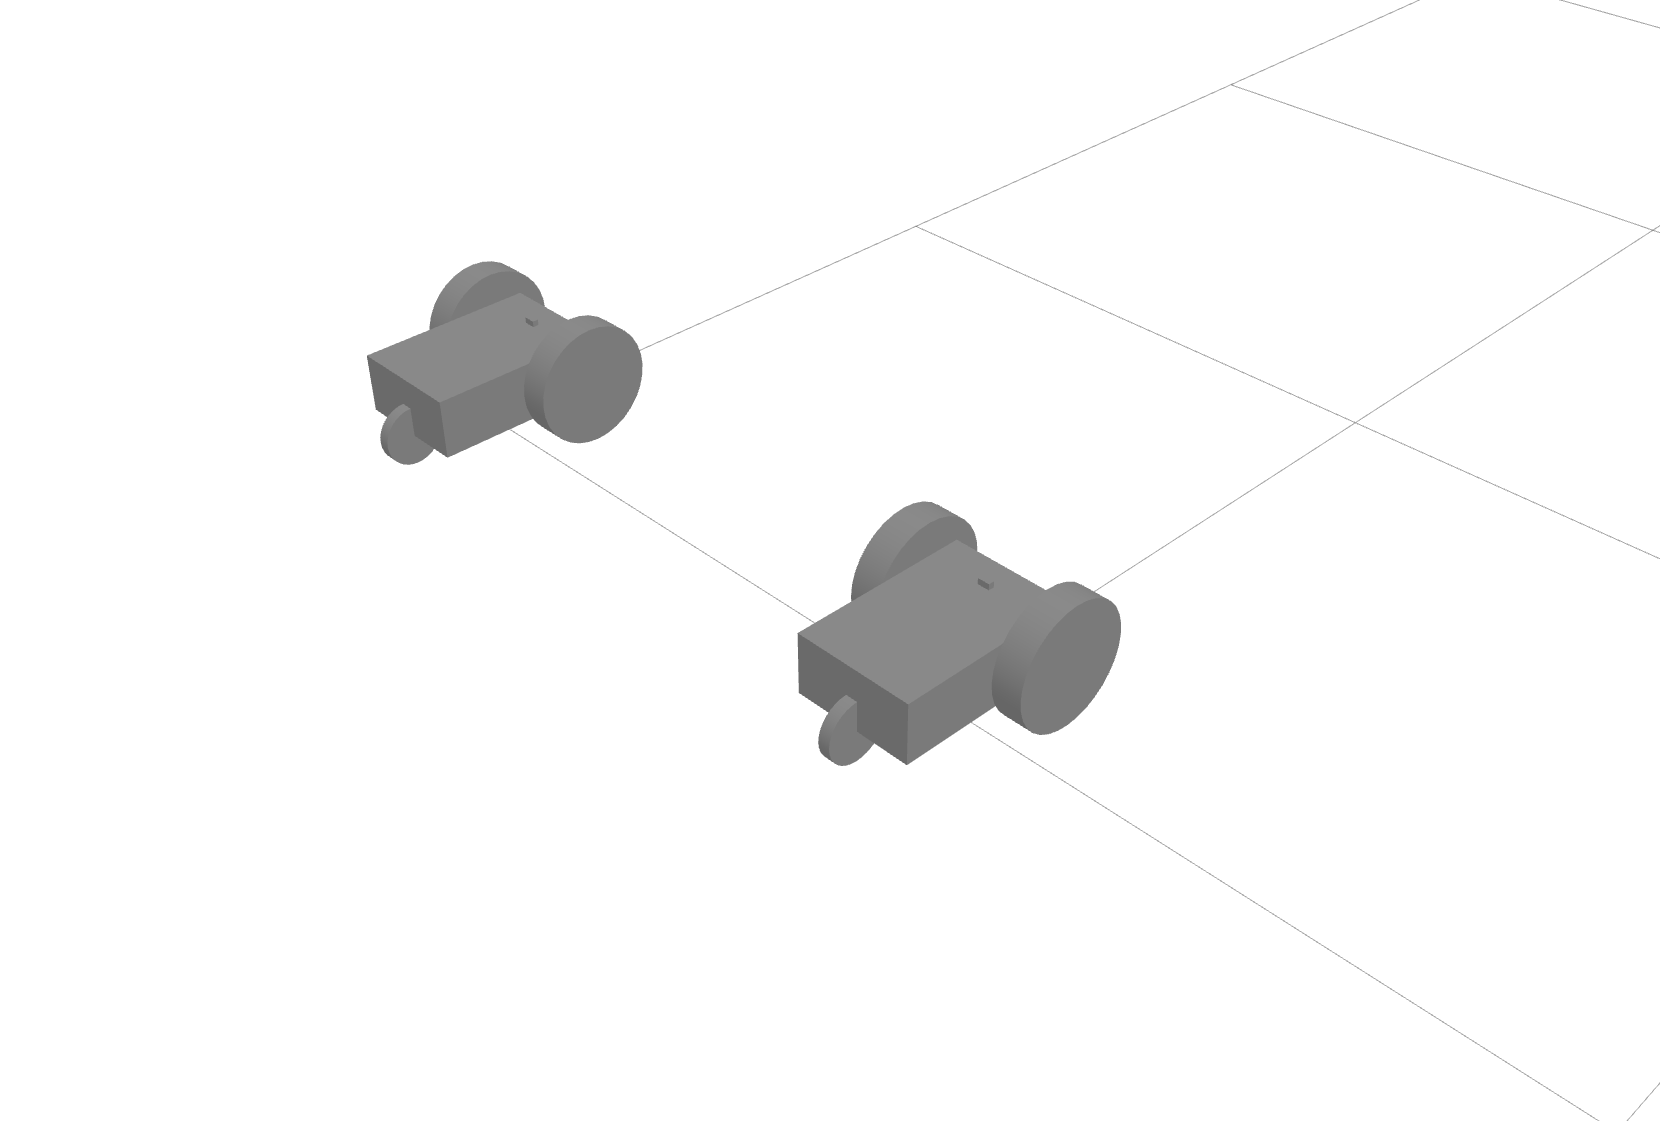
\includegraphics[width=0.5\textwidth]{graphics/crawlers.png}
				\caption{Modèle de crawler utilisé pour l'inspection acoustique de structures métalliques.}
				\label{fig:crawler}
			\end{figure}

			Chaque robot est soit émetteur, soit récepteur, soit les deux.
			Les crawlers sont équipés de différents capteurs.
			Parmi eux :
			\begin{itemize}
				\item un capteur IMU (Inertial Measurement Unit)
				\item un capteur UGW (Ultrasonic Guided Waves)
				\item un capteur LIDAR (Light Detection And Ranging)
			\end{itemize}
			Le capteur IMU permet de connaître l'orientation du robot dans l'environnement.
			Le capteur UGW permet de détecter la présence de corrosion sur la surface métallique en émettant et en recevant des ondes ultrasoniques.
			Le capteur LIDAR permet de détecter les obstacles dans l'environnement.
			Les obstacles considérés ici, sont principalement les différents robots inspectant la surface métallique.
			La détection des zones de corrosion est réalisée par l'émission d'ondes ultrasoniques par un robot et la réception de ces ondes par un autre robot.
			Dans la mesure où l'onde reçue par un des crawlers est altérée, alors il existe un point de corrosion entre le robot émetteur et le robot récepteur.
			La détection de ces zones de corrosion est réalisée en temps réel.
			La portée maximale des ondes ultrasoniques est notée $d_{max}$.
			Nous approximons le temps de propagation des ondes ultrasoniques dans la surface métallique par un temps nul.

			Nous utilisons une grille d'occupation pour modéliser l'environnement dans lequel les robots évoluent lors de l'inspection acoustique des structures métalliques.
			Cette grille nous permet de représenter et de catégoriser les différents états des zones de la surface métallique.
			La grille d'occupation est composée de cellules, où chaque cellule correspond à une petite région de l'environnement.
			En particulier, nous avons utilisé une résolution de 0.05 mètre par cellule.
			Nous utilisons trois états pour caractériser ces cellules : inconnu, vide et occupé.
			L'état inconnu désigne les zones dont l'état n'a pas encore été déterminé ou détecté.
			L'état vide indique les zones où il n'y a pas de corrosion détectée, c'est-à-dire que la surface métallique est saine.
			Enfin, l'état occupé représente les zones de corrosion identifiées, où la présence de défauts ou de détérioration est détectée.

			En utilisant cette grille d'occupation, nous pouvons suivre et mettre à jour en temps réel l'état des différentes zones de la surface métallique pendant l'inspection.
			Cela nous permet de planifier les mouvements des robots, d'optimiser leur trajectoire et d'assurer une couverture complète de la surface à inspecter.
			De plus, cette représentation nous offre une vision claire de l'état de corrosion de la structure métallique, facilitant ainsi l'analyse et l'évaluation des résultats de l'inspection.

			Dans la suite de notre proposition, nous détaillerons les algorithmes et les méthodes utilisées pour mettre à jour la grille d'occupation en fonction des informations recueillies par les capteurs des robots.
			Nous discuterons également des stratégies de navigation multi-robots qui exploitent cette modélisation pour optimiser l'acquisition de données et améliorer l'efficacité de l'inspection acoustique.
		\subsection{Proposition de solution}
			Nous présentons notre proposition de solution pour l'inspection acoustique de structures métalliques en utilisant des stratégies de navigation multi-robots.
			Nous avons développé trois stratégies spécifiques pour optimiser l'acquisition de données et permettre la réalisation de la tomographie des surfaces métalliques.
			Ces trois stratégies sont les suivantes :
			\begin{enumerate}
				\item Stratégie de navigation \textit{peinture au rouleau}
				\item Stratégie de navigation \textit{ski nordique}
				\item Stratégie de navigation \textit{investigation polygonale}
			\end{enumerate}
			Parmi ces stratégies, les deux premières sont non réactives et peuvent être considérées comme des stratégies d'exploration grossières, le but étant de rapidement obtenir une couverture globale de la surface à inspecter.
			La troisième stratégie est réactive et permet d'optimiser l'acquisition de données pour la réalisation de la tomographie.
			Ces trois stratégies ont pour objectif de cartographier la surface métallique et de détecter les zones de corrosion.
			Nous définissons ces trois stratégies de navigation dans les sous-sections suivantes.
			Nous explicitons également comment la structure de données utilisée pour la cartographie des zones de corrosion, une grille d'occupation, est mise à jour en fonction des informations recueillies par les capteurs UGW des robots.
			\subsubsection*{Mise à jour de la grille d'occupation pour la cartographie}
				Lors du balayement de la surface à inspecter par une paire de robot émetteur et récepteur, le robot émetteur émet une onde acoustique dans la structure métallique, qui est ensuite reçue par le robot récepteur.
				La détection étant considérée comme parfaite, le robot récepteur reçoit l'onde émise par le robot émetteur, sans quasi-altération de la puissance du signal, si et seulement si le segment de droite entre les deux robots ne traverse pas une zone de corrosion.
				Il est ainsi possible de déterminer si une zone de corrosion est présente entre les deux robots en vérifiant si le signal reçu par le robot récepteur est suffisamment puissant.
				Dans la mesure où il n'y a pas de détection de corrosion entre l'émetteur et le récepteur, alors le segment de droite entre les deux robots est considéré comme étant libre de corrosion.
				Dans le cas contraire, alors les points du segment de droite entre les deux robots sont considérés comme étant de la corrosion, à l'exception des points préalablement perçus comme étant libre de corrosion.
				On surestime donc la présence de corrosion sur le segment.
				Les stratégies de déplacement viseront à réaliser plusieurs mesures, pour réduire cette surestimation, et approcher la forme réelle de la corrosion.

				Il nous suffit maintenant de déterminer quelles cellules de la grille d'occupation sont traversées par le segment de droite entre les deux robots.
				Pour cela, nous utilisons l'algorithme de tracé de segment de Bresenham~\cite{enwiki:1155124335} qui est couramment utilisé pour déterminer les points d'un plan discret qui doivent être tracés afin de former une approximation de segment de droite entre deux points donnés.
				Nous détaillons notre implémentations de cet algorithme dans la section~\ref{subsec:Bresenham}.

				Lors de l'exploration de la surface métallique, la grille d'occupation est mise à jour en fonction des informations recueillies par les robots.
				Plus précisément, les cellules de la grille d'occupation qui identifient des éléments de corrosion sont mises à jour avec l'état occupé, tandis que les cellules qui identifient des zones saines sont mises à jour avec l'état vide.
				Nous aboutissions ainsi à une grille d'occupation qui représente l'état de corrosion de la surface métallique, avec, pour chaque zone de corrosion, une approximation de l'enveloppe convexe de la zone de corrosion.
			\subsubsection*{Stratégie de navigation \textit{peinture au rouleau}}
				La première stratégie de navigation que nous proposons est la stratégie de navigation \textit{peinture au rouleau}.
				Nous avons choisi ce nom pour cette stratégie, car le mouvement des robots durant cette startégie est similaire à celui d'un rouleau de peinture lors de la peinture d'un mur.
				Cette stratégie repose sur une exploration grossière de la surface à inspecter, où les robots se déplacent en ligne droite sur des trajectoires parallèles, garantissant une couverture globale de la zone d'inspection.
				Il s'agit donc ici d'effectuer un quadrillage de la surface à inspecter.

				\begin{figure}[h!]
					\centering
					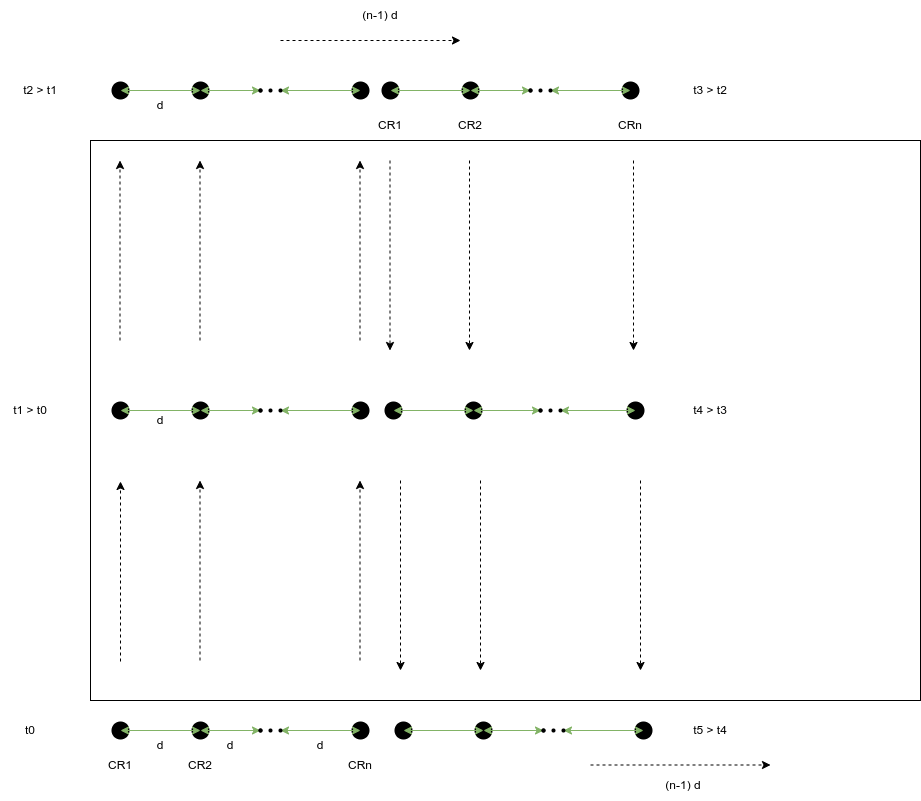
\includegraphics[scale=0.5]{graphics/peinture_au_rouleau.png}
					\caption{Stratégie de navigation \textit{peinture au rouleau}.}
					\label{fig:peinture_au_rouleau}
				\end{figure}

				Nous présentons sur la figure~\ref{fig:peinture_au_rouleau} un schéma décrivant la stratégie de navigation peinture au rouleau.
				Cette stratégie consiste en deux phases, une phase de déplacement vertical et une phase de déplacement horizontal.
				La figure~\ref{fig:peinture_au_rouleau} présente la première phase de déplacement vertical.
				Afin de réaliser cette stratégie, un minimum de, $n \ge 2$ robots, alignés horizontalement et séparés par une distance $d < d_{max}$, est utilisé.
				Ces robots se déplacent verticalement, en simultané, en suivant une trajectoire parallèle.
				Une fois l'extrémité de la surface à inspecter atteinte, les robots effectuent une rotation de 90 degrés et se translatent horizontalement, en simultané, d'une distance $(n - 1) \cdot d$.
				Ils effectuent ensuite une nouvelle rotation de 90 degrés et se déplacent de nouveau verticalement, en ligne droite, en simultané, en suivant une trajectoire parallèle entre eux, jusqu'à atteindre l'autre extrémité de la surface à inspecter.
				Ce procédé est répété jusqu'à ce que la surface métallique soit entièrement inspectée.
				Le même procédé est ensuite répété, mais cette fois-ci, horizontalement.

				Durant cette stratégie, chaque robot est à la fois un émetteur et un récepteur d'ondes UGW.
				Si la distance qui sépare un robot $n_a$ d'un robot $n_b$, $(n_a, n_b) \in \{1, 2, \dots, n\}^2$, est inférieure à la distance maximale de propagation des ondes UGW, $d_{max}$, alors le robot $n_a$ est capable de recevoir le signal émis par le robot $n_b$ et réciproquement.
				Il n'est cependant pas nécessaire pour un robot $n_k$, $n_k \in \{1, 2, \dots, n\}$, de traiter les signaux reçu de tous les autres robots.
				En effet, les robots étant alignés, les signaux reçus des robots $n_{k-1}$ et $n_{k+1}$, sont suffisants pour la reconstruction de l'état de la surface métallique.
				Les ondes émisent par les robots $n_1, n_2, \dots, n_{k-2}$ et $n_{k+2}, \dots, n_n$ ne sont pas utiles pour le robot $n_k$.
				Le robot $n_k$ peut donc ignorer ces signaux et se concentrer uniquement sur les signaux reçus des robots $n_{k-1}$ et $n_{k+1}$.
				Dans la mesure où les premiers signaux perçus par le robot $n_k$ sont ceux émis par les robots $n_{k-1}$ et $n_{k+1}$, du fait de leur proximité, il est possible pour le robot $n_k$ de filtrer les signaux reçus des autres robots.
				Ceci constitue une optimisation en terme de traitement pour chaque robot.

				Le fait que les robots se déplacent en suivant une trajectoire parallèle et en simultané, implique que les rayons du signal émis par le robot émetteur et reçu par le robot récepteur, ont toujours une orientation de $0$ radian pour la phase verticale et une orientation de $\frac{\pi}{2}$ radians pour la phase horizontale.
				Il n'y a donc pas une grande variation de l'orientation du signal émis et reçu.
				Ainsi, cette stratégie ne pourra approcher les enveloppes convexes des zones de corrosion que par des rectangles.
				Des examples de grilles d'occupations résultantes de la stratégie de navigation \textit{peinture au rouleau}, représentées sous formes d'images, où les cellules de la grille correspondent aux pixels des images, sont réprésentés à l'annexe~\ref{annexe:resultat}, figure~\ref{fig:peinture_au_rouleau_resultats}.
			\subsubsection*{Stratégie de navigation \textit{ski nordique}}
				La deuxième stratégie que nous proposons est la stratégie de navigation \textit{ski nordique}.
				Nous avons choisi ce nom pour cette stratégie, car le mouvement des robots durant cette stratégie est similaire au mouvement des skis d'un skieur.
				Cette stratégie consiste toujours en des déplacements en ligne droite et en suivant des trajectoires parallèles, mais cette fois-ci, les robots se déplacent de manière séquentielle et non plus de manière simultanée.
				Dans cette stratégie, nous avons voulu accroître la diversité d'orientation des rayons du signal émis et reçu, afin d'approcher plus précisément les enveloppes convexes des zones de corrosion.

				\begin{figure}[h!]
					\centering
					\begin{subfigure}[t]{0.45\linewidth}
						\centering
						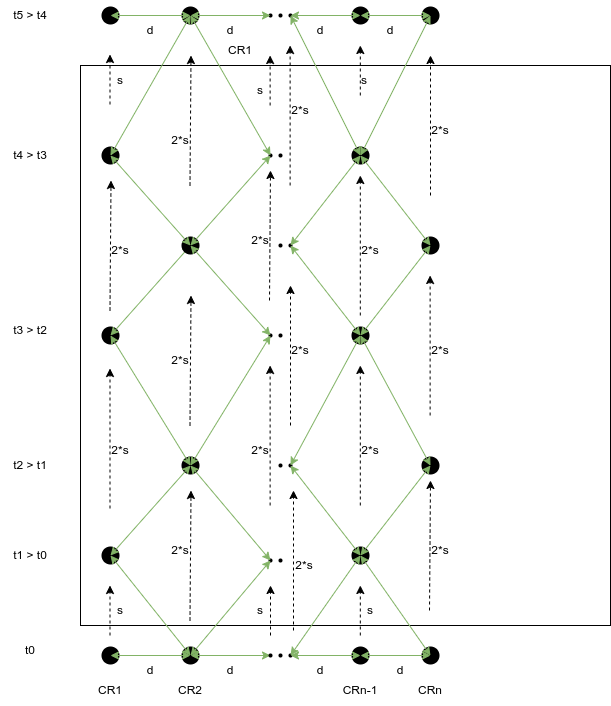
\includegraphics[width=\linewidth]{graphics/ski_nordique_1.png}
						\caption{Stratégie de navigation \textit{ski nordique} - première phase.}
						\label{fig:ski_nordique_1}
					\end{subfigure}
					\hfill
					\begin{subfigure}[t]{0.45\linewidth}
						\centering
						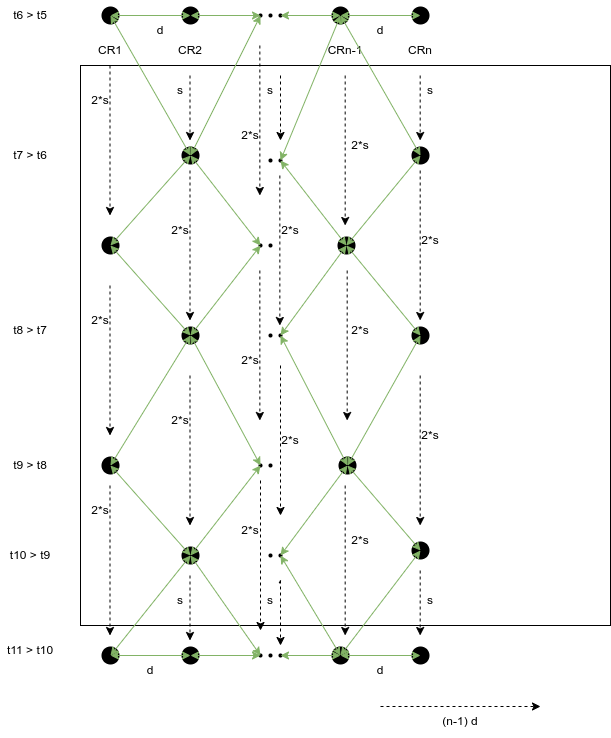
\includegraphics[width=\linewidth]{graphics/ski_nordique_2.png}
						\caption{Stratégie de navigation \textit{ski nordique} - seconde phase.}
						\label{fig:ski_nordique_2}
					\end{subfigure}
					\caption{Stratégie de navigation \textit{ski nordique}.}
					\label{fig:ski_nordique}
				\end{figure}

				La figure~\ref{fig:ski_nordique} présente un schéma décrivant la stratégie de navigation \textit{ski nordique}.
				Cette stratégie consiste également en deux phases, une phase de déplacement vertical et une phase de déplacement horizontal.
				La figure~\ref{fig:ski_nordique} présente la première phase de déplacement vertical.
				Afin de réaliser cette stratégie, un minimum de, $n \ge 2$ robots, alignés horizontalement et séparés par une distance $d < d_{max}$, est utilisé.
				Ces robots se déplacent verticalement, en suivant une trajectoire parallèle, mais de manière séquentielle.
				Les robots impairs se déplacent en ligne droite d'une distance $s$ et s'arrêtent.
				Les robots pairs se déplacent ensuite en ligne droite d'une distance $2 \cdot s$ et s'arrêtent.
				Ce procédé est répété jusqu'à ce que l'extrémité de la surface soit atteinte (figure \ref{fig:ski_nordique_1}).
				Ensuite, les robots répètent ce même procédé, dans le sens inverse et de manière que les points d'arrêt des robots ne soient pas les mêmes que ceux précédemment (figure \ref{fig:ski_nordique_2}).
				C'est-à-dire que cette fois ci, ce sont les robots pairs qui commencent par se déplacer en ligne droite d'une distance $s$ puis s'arrêtent.
				Ce sont ensuite les robots impairs qui se déplacent en ligne droite d'une distance $2 \cdot s$ puis s'arrêtent.
				Les robots se déplacent ensuite horizontalement d'une distance $(n - 1) \cdot d$ et répètent le même procédé jusqu'à ce que la surface métallique soit entièrement inspectée.
				Le même procédé est ensuite répété, mais cette fois-ci, horizontalement.
				Afin que les differents robots receveurs puissent recevoir les signaux émis par les robots émetteurs, il faut également imposer que $s$ soit inférieur strictement à $\frac{d_{max}}{2}$, soit $s < \frac{d_{max}}{2}$.

				Durant cette stratégie, chaque robot est à la fois un émetteur et un récepteur d'ondes UGW.
				Ici, comme pour la stratégie de navigation \textit{peinture au rouleau}, il n'est pas nécéssaire pour un robot $n_k$, $n_k \in \{1, 2, \dots, n\}$, de traiter les signaux reçu par les robots autres que $n_{k-1}$ et $n_{k+1}$.

				Le fait que les robots se déplacent en suivant une trajectoire parallèle, mais de manière séquentielle, implique que les rayons du signal émit par le robot émetteur et reçu par le robot récepteur, ont une orientation d'une plus grande variation.
				Ainsi, cette stratégie permet d'approcher les enveloppes convexes des zones de corrosion par des formes plus diverses et précises que des rectangles.
				Des examples de grilles d'occupations résultantes de la stratégie de navigation \textit{ski nordique}, représentées sous formes d'images, où les cellules de la grille correspondent aux pixels des images, sont réprésentés à l'annexe~\ref{annexe:resultat}, figure~\ref{fig:ski_nordique_resultats} et figure~\ref{fig:ski_nordique_resultats_2}.
			\subsubsection*{Stratégie de navigation \textit{investigation polygonale}}
				La troisième stratégie que nous proposons est la stratégie de navigation \textit{investigation polygonale}.
				Nous avons vu,  précédemment, qu'à l'issue de la réalisation de la stratégie de navigation \textit{peinture au rouleau}, l'enveloppe convexe des zones de corrosion était approximée par un rectangle.
				Cette approximation est un peu plus précise pour la stratégie de navigation \textit{ski nordique}.
				Il serait intéressant d'avoir un plus grand degré de précision autours des zones potentielles de corrosion.
				C'est ce que nous proposons avec la stratégie de navigation \textit{investigation polygonale}.
				Cette stratégie consiste à investiguer autour des zones potentielles de corrosion, détectées au préalable par une des deux stratégies de navigation précédentes.
				Elle consiste à positionner les robots autours des zones de corrosion et à les faire se déplacer en suivant une trajectoire polygonale, de manière que les rayons du signal émis et reçu aient une orientation d'une plus grande variation autour même de ces zones.

				\begin{figure}[h!]
					\centering
					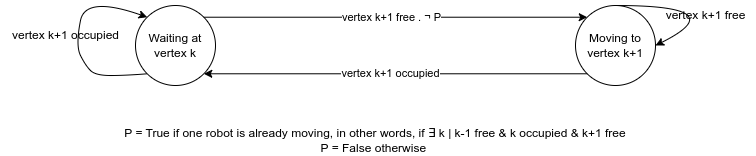
\includegraphics[scale=0.6]{graphics/automat_poly.png}
					\caption{Stratégie de navigation \textit{investigation polygonale}.}
					\label{fig:automat}
				\end{figure}

				Nous présentons sur la figure~\ref{fig:automat} un automate à états finis décrivant la stratégie de navigation \textit{investigation polygonale}.
				Au début de la stratégie de navigation \textit{investigation polygonale}, chaque $n \in \mathbb{N}$ robots de $k \in \mathbb{N}$ équipes sont positionnés sur des sommets consécutifs d'un polygone englobant la zone potentielle de corrosion.
				Dans cette dernière, chaque robot a deux états.
				Le premier consiste à attendre et le second consiste à se déplacer en suivant la trajectoire polygonale, à savoir parcourir les différents sommets constituant le polygone.
				Le robot capable d'avancer, c'est-à-dire, dont le sommet suivant n'est pas occupé par un autre robot, avance.
				Les autres attendent jusqu'à ce que le robot qui est en train d'avancer atteigne le dernier sommet libre du polygone.
				Le procédé est ensuite répété pour chaque robot de chaque équipe jusqu'à ce que les sommets occupés par les robots soient les mêmes que ceux occupés au début de la stratégie de navigation \textit{investigation polygonale}.

				\begin{figure}[h!]
					\centering
					\begin{subfigure}[t]{0.3\linewidth}
						\centering
						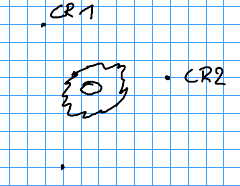
\includegraphics[width=\linewidth]{graphics/triangle_1.png}
						\caption{Phase initiale.}
						\label{fig:triangle_1}
					\end{subfigure}
					\hfill
					\begin{subfigure}[t]{0.3\linewidth}
						\centering
						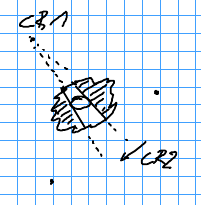
\includegraphics[width=\linewidth]{graphics/triangle_2.png}
						\caption{Première phase de déplacement.}
						\label{fig:triangle_2}
					\end{subfigure}
					\hfill
					\begin{subfigure}[t]{0.3\linewidth}
						\centering
						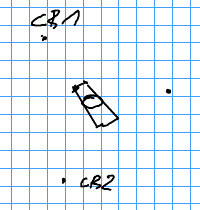
\includegraphics[width=\linewidth]{graphics/triangle_3.png}
						\caption{Seconde phase.}
						\label{fig:triangle_3}
					\end{subfigure}
					\hfill
					\begin{subfigure}[t]{0.3\linewidth}
						\centering
						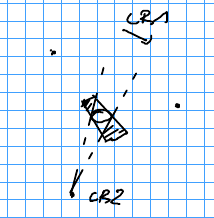
\includegraphics[width=\linewidth]{graphics/triangle_4.png}
						\caption{Seconde phase de déplacement.}
						\label{fig:triangle_4}
					\end{subfigure}
					\hfill
					\begin{subfigure}[t]{0.3\linewidth}
						\centering
						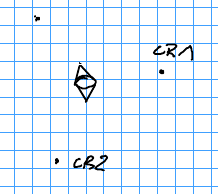
\includegraphics[width=\linewidth]{graphics/triangle_5.png}
						\caption{Troisième phase.}
						\label{fig:triangle_5}
					\end{subfigure}
					\hfill
					\begin{subfigure}[t]{0.3\linewidth}
						\centering
						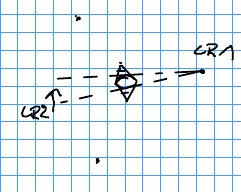
\includegraphics[width=\linewidth]{graphics/triangle_6.png}
						\caption{Troisième phase de déplacement.}
						\label{fig:triangle_6}
					\end{subfigure}
					\hfill
					\begin{subfigure}[t]{0.3\linewidth}
						\centering
						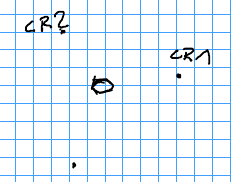
\includegraphics[width=\linewidth]{graphics/triangle_7.png}
						\caption{Dernière phase.}
						\label{fig:triangle_7}
					\end{subfigure}
						\caption{Phases de déplacement de la stratégie de navigation \textit{investigation polygonale}.}
						\label{fig:triangle}
				\end{figure}

				Nous présentons à la figure~\ref{fig:triangle} un exemple des différentes phases de déplacement de la stratégie de navigation \textit{investigation polygonale} avec $k = 1$ équipe, $n = 2$ robots et un poygone à 3 sommets.
				Sur ces différentes figures, nous avons représenté une zone de corrosion par un cercle et une approximation de cette zone par une forme enveloppant le cercle.
				L'objectif est d'approcher le plus finement possible la zone de corrosion.
				La zone de corrosion n'est pas connue à l'avance, seule la forme enveloppant le cercle est connue.
				La figure~\ref{fig:triangle_1} présente la phase initiale de la stratégie de navigation \textit{investigation polygonale}.
				La figure~\ref{fig:triangle_2} présente la première phase de déplacement de la stratégie de navigation \textit{investigation polygonale}, pendant que le crawler $CR2$ avance.
				Nous pouvons voir qu'après que le crawler $CR2$ ait avancé, une partie de la zone suspectée comme étant de la corrosion est éliminée et considérée comme seine, comme nous pouvons le voir à la figure~\ref{fig:triangle_3}.
				Les crawlers continuent de se déplacer jusqu'à atteindre leur position initiale, comme nous pouvons le voir à la figure~\ref{fig:triangle_7}.

				\begin{Definition}[Zone fantôme]
					\label{def:fantomas}
					Une zone fantôme est une zone de corrosion détectée par une des stratégies de navigation, mais qui n'est pas une zone de corrosion. Il s'agit d'un faux positif.
				\end{Definition}

				La stratégie de navigation \textit{investigation polygonale} a deux avantages.
				Le premier est qu'elle permet de rapidement éliminer les zones fantômes~\ref{def:fantomas}.
				Le second est qu'elle permet d'approcher les enveloppes convexes des zones de corrosion par des formes plus diverses et précises que des rectangles du fait de la grande variation de l'orientation des rayons du signal émis et reçu par les robots autour de chaque sommet du polygone.

				Cette stratégie nécessite deux étapes préalables à son exécution :
				\begin{enumerate}
					\item l'extraction des zones de corrosion détectées par une des stratégies de navigation précédentes.
					\item la détermination de l'ordre d'investigation des zones de corrosion.
				\end{enumerate}

				La première étape peut être résolue en utilisant un algorithme de décomposition de graphe en composantes fortement connexes.
				Une composante fortement connexe est définie à la définition~\ref{def:scc}.
				Nous considérons alors notre grille d'occupation, résultante de l'exploration d'une des deux stratégies définies préalablement, comme un graphe non orienté $G = (V, E)$, où  $V$ est l'ensemble des sommets du graphe, correspondant aux cellules de la grille d'occupation et $E$ sont les arêtes du graphe, correspond aux cellules adjacentes.
				Ce problème est bien connu et il existe des algorithmes simples pour les résoudre comme l'algorithme de Tarjan~\cite{enwiki:1148118528}, de complexité temporelle linéaire $O(|V| + |E|)$.
				Nous ne nous pencherons pas plus sur ce problème et confions sa résolution à la bibliothèque \textit{OpenCV}.

				\begin{Definition}[Composante fortement connexe (SCC)]
					\label{def:scc}
					Une composante fortement connexe d'un graphe $G = (V, E)$ est un sous-ensemble $C$ de $V$ tel que pour tout couple de sommets $(u, v) \in C^2$, il existe un chemin de $u$ à $v$ et un chemin de $v$ à $u$.
				\end{Definition}

				\begin{Definition}[Cycle hamiltonien]
					\label{def:hamilton}
					Un cycle hamiltonien est un cycle passant par tous les sommets d'un graphe, une et une seule fois.
				\end{Definition}

				\begin{Definition}[Problème du voyageur de commerce (TSP)]
					\label{def:tsp}
					Étant donné un graphe $G = (V, E)$, où $V$ est l'ensemble des sommets du graphe et $E$ est l'ensemble des arêtes du graphe, et une fonction de coût $c : E \rightarrow \mathbb{R}$, le problème du voyageur de commerce consiste à trouver un cycle hamiltonien~\ref{def:hamilton} de coût minimal dans $G$.
				\end{Definition}

				\begin{Definition}[Problème du voyageur de commerce multiple avec multiples dépôts (mTSP)]
					\label{def:mtsp}
					Étant donné un graphe $G = (V, E)$, où $V$ est l'ensemble des sommets du graphe et $E$ est l'ensemble des arêtes du graphe, une fonction de coût $c : E \rightarrow \mathbb{R}$, et un ensemble de dépôts $D \subset V$, le problème du voyageur de commerce multiple avec multiples dépôts consiste à trouver un ensemble de cycles de coût total minimal dans $G$, chacun passant par un et un seul dépôt.
				\end{Definition}

				La seconde étape peut être résolue en utilisant un algorithme de TSP~\ref{def:tsp} (\textit{Travelling Salesman Problem}) dans le cas où le nombre d'équipes $k$ est égale à 1 et un algorithme de mTSP~\ref{def:mtsp} (\textit{(multiple depot) multiple Travelling Salesman Problem}) dans le cas où le nombre d'équipes $k$ est supérieur strictement à 1.
				Il existe plusieurs paradigmes de résolution pour résoudre ce type de problème.
				Un premier est de trouver une solution exacte en utilisant un algorithme de programmation linéaire en nombres entiers.
				Un second est de trouver une solution approchée en utilisant une méta-heuristique.

				\begin{Definition}[Classe NP]
					\label{def:np}
					La classe NP est la classe des problèmes de décision qui peuvent être résolus par un algorithme non-déterministe en temps polynomial.
				\end{Definition}

				\begin{Definition}[Problème NP-difficile]
					\label{def:nph}
					Un problème est NP-difficile s'il est au moins aussi difficile que les problèmes de la classe NP.
					En d'autres termes, un problème est NP-difficile s'il existe un algorithme de réduction polynomiale qui transforme un problème de la classe NP en une instance de ce problème.
				\end{Definition}

				\begin{Definition}[Problème NP-complet]
					\label{def:npc}
					Un problème est NP-complet s'il est à la fois NP et NP-difficile.
				\end{Definition}

				Le problème du voyageur de commerce est un problème NP-complet~\ref{def:npc}.
				Il peut être traité comme un problème d'optimisation linéaire en nombres entiers~\cite{article244, gurobi25}.
				Pour ce faire, nous utilisons la formulation présentée à l'équation~\ref{eq:tsp}.

				\begin{equation}
					\label{eq:tsp}
					\begin{array}{ll@{}rr}
						\text{minimiser} &
						\displaystyle\sum\limits_{i \in V} \sum\limits_{j \in V} c_{ij} x_{ij} &
						&
						\\
						\text{soumis à} &
						\displaystyle\sum\limits_{i \in V} x_{ij} = 1 &
						&
						\forall j \in V \\
						&
						\displaystyle\sum\limits_{j \in V} x_{ij} = 1 &
						&
						\forall i \in V \\
						&
						\displaystyle\sum\limits_{i \in S} \sum\limits_{j \in S} x_{ij} \leq |S| - 1 &
						&
						\forall S \subset V, 2 \leq |S| \leq |V| - 1 \\
						&
						x_{ij} \in \{0, 1\} &
						&
						\forall i \in V, \forall j \in V \\
					\end{array}
				\end{equation}

				La fonction objectif à minimiser de la formulation~\ref{eq:tsp} est la somme des distances entre chaque paire de villes.
				Les deux premières contraintes assurent que chaque ville est visitée exactement une fois.
				La troisième contrainte assure que le cycle formé par les villes visitées est simple, c'est-à-dire, qu'il ne contient pas de sous-cycles.
				La dernière contrainte assure que les variables de décision $x_{ij}$ sont binaires, avec $x_{ij} = 1$ si le robot se déplace de la ville $i$ à la ville $j$ et $x_{ij} = 0$ sinon.

				Le problème du voyageur de commerce multiple avec multiples dépôts est un problème NP-difficile~\ref{def:nph}~\cite{SUNDAR201639}.
				Celui-ci peut être résolu en utilisant une méta-heuristique comme un algorithme génétique~\cite{SinghMTSP, Kiraly2011}

				Dans les prochaines sections, nous détaillerons chaque stratégie de navigation, en exposant les algorithmes et les mécanismes spécifiques utilisés pour mettre en œuvre notre proposition de solution. Nous analyserons également les performances et les résultats obtenus à travers des expérimentations et des évaluations approfondies.
		\subsection{Étude théorique de propriétés de la solution proposée}
			\subsubsection*{Stratégie de navigation \textit{ski nordique}}
				\begin{Proposition}
					L'angle du signal émis et reçu par les robots, pour la stratégie de navigation \textit{ski nordique}, varie entre $-\tan^{-1}(\frac{s}{d})$ et $\tan^{-1}(\frac{s}{d})$.
					\label{prop:angle_ski_nordique}
				\end{Proposition}

				Nous pouvons observer le résultat de la proposition~\ref{prop:angle_ski_nordique}, en nous appuyant sur les propriétés de trigonométrie et la définition de la fonction tangente.
				Nous explicitons sur la figure~\ref{fig:angle_ski_nordique} la démarche entreprise pour trouver $\alpha = -\tan^{-1}(\frac{s}{d})$.
				Cette proposition nous permet de quantifier la porté de l'orientation du signal émis et reçu par les robots.

				\begin{figure}[h!]
					\centering
					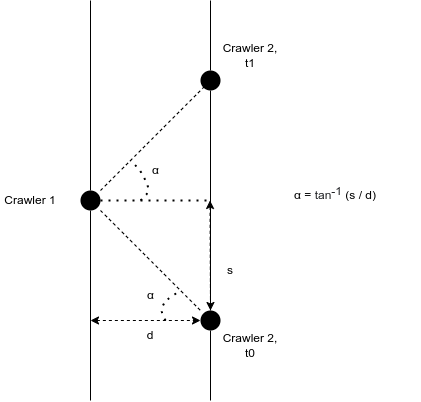
\includegraphics[scale=0.5]{graphics/angle_ski_nordique.png}
					\caption{Orientation du signal émis et reçu pour la stratégie de navigation \textit{ski nordique}.}
					\label{fig:angle_ski_nordique}
				\end{figure}
			\subsubsection*{Stratégie de navigation \textit{investigation polygonale}}
				\begin{Proposition}
					La stratégie de navigation \textit{investigation polygonale}, définie par un polygone, $P$ permet de couvrir tous points à l'intérieur du polygone $P$.
					\label{prop:completude}
				\end{Proposition}
				\begin{proof}
					Démontrons la proposition~\ref{prop:completude}.
					\begin{itemize}
						\item Soit $P$ un polygone convexe à $p$ sommets utilisé pour la stratégie de navigation \textit{investigation polygonale}.
						\item Par simplicité, nous considérons une stratégie à 2 robots, mais la preuve reste semblablement la même pour $n > 2$ robots.
						\item Considérons le robot $r_1$ au sommet $s_1$ du polygone $P$ et le robot $r_2$ au sommet $s_2$ du polygone $P$.
						\item Soit un point $p$ à l'intérieur du polygone $P$.
						\item Alors, il existe un point $p'$ tel que $p$ est sur le segment $[s_1, p']$ et $p'$ est sur le bord du polygone $P$, par définition de la convexité de $P$.
						\item Par définition de la stratégie de navigation \textit{investigation polygonale}, le robot $r_2$ se déplace sur les contours du polygone $P$ et donc en particulier sur le point $p'$.
						\item On a donc pour tout point $p$ à l'intérieur du polygone $P$, il existe un couple de positions pour les robots $r_1$ et $r_2$ tel que $p$ se trouve sur le segment formé par les points où se trouvent les robots $r_1$ et $r_2$.
						\item Donc tous les points à l'intérieur du polygone $P$ sont couverts par la stratégie de navigation \textit{investigation polygonale}.
					\end{itemize}
				\end{proof}

				\begin{Proposition}
					L'approximation de l'enveloppe convexe des zones de corrosion à l'issue de l'investigation polygonale, avec un polygone à $p$ sommets, $p \in \mathbb{N}$, est un polygone d'au plus $2p$ sommets.
					\label{prop:cotes_poly}
				\end{Proposition}
				\begin{proof}
					Donnons une intution de la preuve de la proposition~\ref{prop:cotes_poly}.
					\begin{itemize}
						\item On a, pour chaque sommet du polygone, il existe deux droites passant par ce point et touchant la zone de corrosion sans la traverser.
						\item On a donc, pour un sommet du polygone, au plus deux droites qui participent à la construction de l'approximation de l'enveloppe convexe et donc, dont un segment de ces droites est une arête de l'approximation de l'enveloppe convexe.
						\item On a donc, pour un sommet du polygone, au plus deux arêtes de l'approximation de l'enveloppe convexe.
						\item On a donc, pour un polygone à $p$ sommets, au plus $2p$ arêtes de l'approximation de l'enveloppe convexe.
						\item On a donc, pour un polygone à $p$ sommets, au plus $2p$ sommets de l'approximation de l'enveloppe convexe.
					\end{itemize}
				\end{proof}

				\begin{Conjecture}
					Si le polygone utilisé lors de l'investigation polygonale est un cercle, alors l'approximation de l'enveloppe convexe de la zone de corrosion à l'issue de l'investigation polygonale est l'enveloppe convexe.
					\label{prop:cercle}
				\end{Conjecture}
	\section{Implémentations des algorithmes}
		Dans cette section, nous mettons en évidence certaines des différentes implémentations techniques que nous avons développées pour soutenir nos solutions de navigation et de contrôle multi-robots dans le contexte de l'inspection acoustique de structures métalliques.
		Nous commençons par décrire notre adaptation de l'algorithme de tracé de segment de Bresenham~\cite{enwiki:1155124335}, largement utilisé pour déterminer quels sont les points d'un plan discret qui doivent être tracés afin de former une approximation de segment de droite entre deux points donnés.
		Ensuite, nous abordons l'implémentation de l'algorithme \textit{peinture au rouleau}, qui permet aux robots de se déplacer de manière simultanée, en suivant des trajectoires parallèles.
		Nous poursuivons avec l'implémentation de l'algorithme \textit{ski nordique}, qui permet aux robots de se déplacer de manière alternée, en suivant des trajectoires parallèles, modifiant ainsi l'orientation du vecteur représentant la direction de déplacement de l'onde émise et reçue par la paire de robot.
		De plus, nous examinons l'implémentation de l'algorithme \textit{investigation polygonale}, qui permet aux robots d'examiner plus précisément des zones suspectes de corrosion.
		Enfin, nous présentons l'algorithme de calcul du $\kappa$ de Cohen~\cite{enwiki:1130024730}, utilisé pour évaluer la qualité et la fiabilité des résultats de l'inspection acoustique.
		Nous discutons en détail de notre implémentation de cet algorithme, qui fournit des mesures quantitatives pour évaluer la performance des robots dans l'inspection des structures métalliques.
		Chacune de ces implémentations techniques contribue à l'efficacité et à la précision de notre approche de navigation et de contrôle multi-robots, et sera examinée en détail dans les sous-sections suivantes.
		\subsection*{Algorithme de tracé de segment de Bresenham}\label{subsec:Bresenham}
			\begin{algorithm}[h!]
				\caption{Processus de mise à jour de la grille d'occupation à l'aide de l'algorithme de tracé de segment de Bresenham.}
				\label{alg:Bresenham}
				\KwData{$P_1 \in \mathbb{R}^2$, $P_2 \in \mathbb{R}^2$, $pw \in \mathbb{R}$, $threshold \in \mathbb{R}$, $G$: $l \times w \rightarrow [\text{UNKNOWN}, \text{EMPTY}, \text{OCCUPIED}]$, $l \in \mathbb{N}$, $w \in \mathbb{N}$ \\
					with $P_1$ and $P_2$ the two points to connect, $pw$ the power of the UGW, $threshold$ the threshold above which the power of the UGW is considered undistributed and $G$ the grid to update.}
				\KwResult{The updated grid.}
				$p_0 \gets \text{from\_position\_to\_grid\_coordinate}(P_1)$ \\
				$p_1 \gets \text{from\_position\_to\_grid\_coordinate}(P_2)$ \\
				\If{\text{is\_out\_of\_grid}($p_0$) \textbf{or} \text{is\_out\_of\_grid}($p_1$)}{
					\Return
				}
				$dx \gets p_1.x - p_0.x$ \\
				$dy \gets p_1.y - p_0.y$ \\
				$sx \gets \text{sign}(dx)$ \\
				$sy \gets \text{sign}(dy)$ \\
				$err = dx - dy$ \\
				\While{$p_0 \neq p_1$}{
					\If{$pwd \leq threshold$ \textbf{and} $G(p_0) = \text{UNKNOWN}$}{
						$G(p_0) \gets \text{OCCUPIED}$
					}
					\ElseIf{$pwd > threshold$}{
						$G(p_0) \gets \text{EMPTY}$
					}
					$e2 \gets 2 \times err$ \\
					\If{$e2 > -dy$}{
						$err \gets err - dy$ \\
						$p_0.x \gets p_0.x + sx$
					}
					\If{$e2 < dx$}{
						$err \gets err + dx$ \\
						$p_0.y \gets p_0.y + sy$
					}
				}
			\end{algorithm}

			Nous utilisons l'algorithme de tracé de segment de Bresenham pour déterminer les points du segment de droite entre les deux robots.
			L'algorithme est présenté à l'algorithme~\ref{alg:Bresenham}.
			La partie adaptée à notre problème se trouve entre les lignes 12 et 17 de ce dernier.
			À cet endroit, nous vérifions si la puissance du signal est suffisamment altérée et si le point du segment de droite entre les deux robots n'a pas déjà été perçu comme étant libre de corrosion.
			Si c'est le cas, alors le point considéré est marqué comme étant de la corrosion, modélisé par la valeur \texttt{OCCUPIED}.
			Si la puissance du signal n'est pas suffisamment altérée, alors le point considéré est marqué comme étant libre de corrosion, modélisé par la valeur \texttt{EMPTY}.
			Une fois que tous les points du segment ont été parcourus, la grille $G$ est mise à jour avec les nouvelles informations.
			L'algorithme de tracé de segment de Bresenham contribue ainsi à la construction de la grille d'occupation qui permet de localiser les zones de corrosion détectées par les robots lors de l'inspection acoustique des structures métalliques.
		\subsection*{Algorithme \textit{peinture au rouleau} et \textit{ski nordique}}
			Nous présentons dans cette sous-section les implémentations des algorithmes \textit{peinture au rouleau} et \textit{ski nordique}.
			Leur code source est disponible sur GitLab, ici\footnote{\url{https://gitlab.georgiatech-metz.fr/bugwright2/bugwright2-ws/blob/cr_nav_strat/bugwright_ws/src/floor_nav/missions/peinture_au_rouleau.py}} et ici\footnote{\url{https://gitlab.georgiatech-metz.fr/bugwright2/bugwright2-ws/blob/cr_nav_strat/bugwright_ws/src/floor_nav/missions/ski_nordique.py}}.

			Les implémentations de ces algorithmes, ont été réalisées en utilisant le langage de programmation Python et les bibliothèques ROS (Robot Operating System).
			Dans ces implémentations, nous utilisons le framework ROS Task Manager~\cite{ROSTaskManager} pour gérer les tâches des robots inspecteurs.
			Tout d'abord, nous initialisons le nœud ROS et créons un client de tâches.
			Ensuite, nous récupérons les paramètres nécessaires tels que la vitesse des crawlers, l'identifiant du crawler, la distance entre les crawlers, le chevauchement ou encore les dimensions de la surface à inspecter.

			Les algorithmes sont ensuite exécutés en suivant une séquence de mouvements précis.
			Pour chaque crawler, nous définissons des trajectoires verticales et horizontales en utilisant une boucle itérative et des calculs mathématiques. Les crawlers se déplacent le long des trajectoires définies, en utilisant les fonctions du client de tâches telles que \texttt{AlignWithTarget} et \texttt{FollowLine} pour maintenir une trajectoire précise.

			Pendant l'exécution des algorithmes, les crawlers se synchronisent en utilisant les fonctions \texttt{SetStatusSync} et \texttt{WaitForStatusSync} du client de tâches.
			Cela garantit que les crawlers exécutent les mouvements de manière coordonnée et se positionnent correctement pour couvrir toute la surface métallique.
			À la fin de chaque étape de mouvement, le statut est mis à jour et la synchronisation est effectuée avec le partenaire correspondant.

			L'implémentation des deux algorithmes \textit{peinture au rouleau} et \textit{ski nordique} permettent aux crawlers d'explorer la surface métallique de manière méthodique et complète.
			En utilisant des trajectoires verticales et horizontales, les crawlers parcourent la surface en chevauchant les zones précédemment inspectées pour s'assurer d'une couverture optimale.
			Ici, nous avons utilisé un chevauchement de 10 cm entre les différentes trajectoires verticales et horizontales.

			Une fois les algorithmes terminés, le temps d'exécution est enregistré, fournissant une indication de la durée nécessaire pour inspecter la surface métallique.
			La grille d'occupation est également enregistrée afin de calculer le score de l'inspection.
			Cette implémentation constitue une étape essentielle dans notre proposition de solution pour l'inspection acoustique de structures métalliques et permet de garantir une couverture complète et efficace de la surface à inspecter.
		\subsection*{Algorithme \textit{investigation polygonale}}
			Nous présentons dans cette sous-section l'implémentation de l'algorithme \textit{investigation polygonale}.
			Le code source correspondant est disponible sur GitLab~\footnote{\url{https://gitlab.georgiatech-metz.fr/bugwright2/bugwright2-ws/blob/cr_nav_strat/bugwright_ws/src/floor_nav/missions/investigation_polygonale.py}}.

			L'implémentation de cet algorithme, a également été réalisée en utilisant le langage de programmation Python et les bibliothèques ROS (Robot Operating System).
			Dans cette implémentation, nous utilisons toujours le framework ROS Task Manager~\cite{ROSTaskManager} pour gérer les tâches des robots inspecteurs.
			Premièrement, nous initialisons le nœud ROS et récupérons les différents paramètres et plus particulièrement la carte des zones potentielles de corrosion, sur laquelle nous nous basons pour l'inspection, qui sont issues d'une des deux stratégies grossières.
			Ensuite, nous extrayons les composantes fortement connexes de la carte en utilisant la fonction \texttt{connectedComponentsWithStats} de la biblliothèque \textit{OpenCV}.
			Cette fonction utilise l'algorithme spaghetti de Bolleli~\cite{BolelliSpaghetti} pour extraire les composantes fortement connexes d'une image.
			Pour chacune de ces composantes, nous récupérons son centre et ses dimensions.
			Ensuite, nous construisons un polygone à $p \in \mathbb{N}$ côtés autour de chaque centre d'une composante.
			Pour ce faire, nous plaçons $p$ points sur une ellipse centrée sur le centre de la composante et dont les axes sont les dimensions de la composante.
			Nous avons donc pour chaque zone potentielle de corrosion un polygone à $p$ côtés qui l'entoure.
			Il ne reste plus qu'à trouver le plus court chemin qui passe par tous les polygones.
			Pour cela, nous utilisons la bibliothèque \textit{Gurobi} pour résoudre un simple TSP dans le cas où le nombre d'équipes de robots $k = 1$.
			Lorsque $k > 1$, nous utilisons l'algorithme génétique proposé par Elad Kivelevitch~\cite{MDMTSPV_GA} pour résoudre le problème du mTSP avec plusieurs dépôts.

			Une fois les algorithmes terminés, le temps d'exécution est enregistré, fournissant une indication de la durée nécessaire pour inspecter les différentes zones potentielles de corrosion.
			La grille d'occupation est également enregistrée afin de calculer le score de l'inspection.
			Cette implémentation constitue une étape essentielle dans notre proposition de solution pour l'inspection acoustique de structures métalliques et permet d'investiguer les zones potentielles de corrosion de manière efficace.
		\subsection*{Algorithme de calcul du $\kappa$ de Cohen}
			L'évaluation de la qualité et de la fiabilité des résultats de l'inspection acoustique est essentielle pour garantir des mesures précises de l'état des structures métalliques.
			Dans cette sous-section, nous présentons l'algorithme du calcul du $\kappa$ de Cohen~\cite{enwiki:1130024730}, présenté à l'algorithme~\ref{alg:Cohen_Kappa}, une mesure statistique couramment utilisée pour évaluer l'accord entre les résultats obtenus par les robots et une référence humaine.

			\begin{table}[h!]
				\centering
				\begin{tabular}{|c|c|}
					\hline
					$\kappa$ & Interprétation \\
					\hline
					$< 0$ & Désaccord \\
					\hline
					$0.00 - 0.20$ & Accord très faible \\
					\hline
					$0.21 - 0.40$ & Accord faible \\
					\hline
					$0.41 - 0.60$ & Accord modéré \\
					\hline
					$0.61 - 0.80$ & Accord fort \\
					\hline
					$0.81 - 1.00$ & Accord presque parfait \\
					\hline
				\end{tabular}
				\caption{Interprétation du $\kappa$ de Cohen selon Landis et Koch.}
				\label{tab:Kappa_Cohen}
			\end{table}

			L'algorithme de calcul du $\kappa$ de Cohen se base sur la notion de concordance et de discordance entre les résultats des inspections réalisées par les robots et celles réalisées par des inspecteurs humains (vérité de terrain).
			Il prend en compte les résultats positifs, négatifs, faux positifs et faux négatifs obtenus lors de l'inspection acoustique.
			Ces informations sont utilisées pour calculer la valeur du coefficient de Cohen, noté $\kappa$, avec $\kappa = \frac{p_o - p_e}{1 - p_e}$, où $p_o$ est le taux d'accord observé et $p_e$ le taux d'accord attendu.

			\begin{algorithm}[h!]
				\caption{Algorithme du $\kappa$ de Cohen.}
				\label{alg:Cohen_Kappa}
				\KwData{$I_0$: $l \times w \times 3 \rightarrow [0 .. 255]$, $I$: $l \times w \times 3 \rightarrow [0 .. 255]$, $l \in \mathbb{N}$, $w \in \mathbb{N}$ \\
					with $I_0$ the ground truth image and $I$ the image to score.}
				\KwResult{$\kappa \in [0, 1]$}
				$TP \gets 0$ \\
				$TN \gets 0$ \\
				$FP \gets 0$ \\
				$FN \gets 0$ \\
				\For{$i \gets 1$ \KwTo $l$}{
					\For{$j \gets 1$ \KwTo $w$}{
						\If{$\text{is\_label\_1}(I_0(i, j))$}{
							\If{$\text{is\_label\_1}(I(i, j))$}{
								$TP \gets TP + 1$
							}
							\Else{
								$FN \gets FN + 1$
							}
						}
						\Else{
							\If{$\text{is\_label\_1}(I(i, j))$}{
								$FP \gets FP + 1$
							}
							\Else{
								$TN \gets TN + 1$
							}
						}
					}
				}
				$f_c \gets \frac{(TN + FN) (TN + FP) + (FP + TP) (FN + TP)}{TP + TN + FN +FP}$ \\
				$\kappa \gets \frac{TP + TN - f_c}{TP + TN + FN + FP - f_c}$
			\end{algorithm}

			L'algorithme se déroule en plusieurs étapes.
			Tout d'abord, les résultats des inspections réalisées par les robots et les réelles répartitions des zones de corrosion sont comparés pour chaque zone inspectée.
			Pour ce faire, nous comparons les valeurs de chaque cellule de la grille d'occupation, obtenue à l'issue de l'inspection par les robots, avec celles de la vérité terrain.
			Ayant modélisé les différents environnements de tests, nous connaissons la véritable répartition des zones de corrosion.
			Ensuite, les résultats sont regroupés en quatre catégories : concordance positive, concordance négative, discordance positive (faux positifs) et discordance négative (faux négatifs).
			Ces catégories sont utilisées pour calculer les taux d'observation et d'accord observés entre les robots et la véritable répartition des zones de corrosion.
			Le $\kappa$ de Cohen est ensuite calculé à partir des taux d'observation et d'accord observés, prenant en compte la possibilité de concordance due au hasard.
			Plus le $\kappa$ de Cohen se rapproche de 1, plus il y a un accord élevé entre les résultats des robots et ceux de la vérité terrain.
			En revanche, un $\kappa$ proche de 0 indique un faible niveau d'accord, tandis qu'un $\kappa$ négatif suggère une discordance entre les résultats.
			Une Interprétation du $\kappa$ de Cohen selon Landis et Koch est présentée dans le tableau~\ref{tab:Kappa_Cohen}.

			Nous avons implémenté cet algorithme dans le cadre de notre projet, en utilisant les résultats des inspections acoustiques effectuées par les robots et des cartes composées de zones de corrosion comme base de comparaison.
			Cette implémentation nous permet d'obtenir des mesures quantitatives pour évaluer la performance de notre approche de navigation et de contrôle multi-robots dans l'inspection des structures métalliques.
			Dans les prochaines sections, nous détaillerons les résultats obtenus grâce à l'application de cet algorithme du calcul du $\kappa$ de Cohen.
	\section{Expérimentations, validations et évaluations}
		Dans cette section, nous présentons les expérimentations que nous avons menées pour valider et évaluer nos différentes stratégies de navigation et de contrôle multi-robots dans le contexte de l'inspection acoustique de structures métalliques.
		Ces expérimentations visent à démontrer l'efficacité, la précision et la fiabilité de notre système dans la détection et la localisation des zones de corrosion.

		Pour mener à bien ces étapes, nous avons choisi d'effectuer nos expériences en utilisant \textit{Gazebo}, un environnement de simulation bien établi dans le domaine de la robotique.
		Nous avons commencé par construire plusieurs cartes de tests.
		Ces cartes modélisent une surface plane sur laquelle sont placées des formes géométriques simples, des rectangles et des cercles, et des formes plus complexes, des polygones entre 3 et 8 sommets.
		Ces différentes formes géométriques représentent les zones de corrosion que nous souhaitons détecter et localiser.
		Nous présentons en annexe~\ref{annexe:cartes}, sur la figure~\ref{fig:test_models} les cartes que nous avons construites pour nos expérimentations.
		Chacune de ces cartes est de taille 6 mètres par 6 mètres.
		Le nombre de zones de corrosion varie entre 5, 8, 11, 15, 20 et 30 zones.
		La taille et l'emplacement des zones de corrosion sont générés aléatoirement.
		Pour les cartes de 5, 8, 11 et 15 zones, nous avons généré 5 cartes différentes afin d'avoir des résultats plus représentatifs.
		Nous ne nous sommes pas permis de générer plusieurs cartes pour les cartes de 20 et 30 zones, le temps d'investigation polygonale étant trop conséquent.

		Nous avons également simulé le capteur UGW en exploitant la simulation d'un capteur UWB.
		Ce capteur UWB permet d'émettre une impulsion et de la recevoir.
		En mesurant la puissance du signal, sous sommes en mesure de savoir si le signal a traversé un objet ou non.
		Le comportement de ce capteur UWB est donc similaire à celui du capteur UGW, à savoir qu'il permet de détecter la présence d'un objet entre deux points, mais pas de le localiser.

		Nous avons évalué les performances des trois stratégies de navigation en termes de $\kappa$ de Cohen et de temps d'inspection.
		Pour la stratégie \textit{peinture au rouleau} et \textit{ski nordique}, nous avons uniquement utilisé deux robots.
		Pour ces deux stratégies, nous avons fait varier la distance $d$ entre les robots.
		Pour la stratégie \textit{ski nordique}, nous avons également fait varier le pas $s$ entre les robots.
		Pour la stratégie \textit{investigation polygonale}, nous faisons varier le nombre de robots $n$, le nombre d'équipes $k$ et le nombre de côtés $p$ des polygones utilisés.
		Nous utilisons le résultat de la stratégie de navigation \textit{peinture au rouleau} comme point de départ.
		Nous justifions ce choix par le fait que cette stratégie est la plus rapide et la moins précise et donc, la plus susceptible de bénéficier d'une amélioration de la part de la stratégie \textit{investigation polygonale}, sans atteindre des temps d'inspection trop longs.
		Nous faisons donc varier le paramètre $d$ de cette stratégie.
		Nous résumons les paramètres expérimentaux utilisés pour chaque stratégie dans le tableau~\ref{tab:exp_params}.

		\begin{table}[h!]
			\centering
			\begin{tabular}{|c|c|c|}
				\hline
				Stratégie & Paramètre & Valeurs \\
				\hline
				\multirow{2}{*}{\textit{peinture au rouleau}} & $n$ & 2 \\
				& $d$ & 1, 2, 3, 6 (mètres) \\
				\hline
				\multirow{3}{*}{\textit{ski nordique}} & $n$ & 2 \\
				& $d$ & 1, 2, 3, 6 (mètres) \\
				& $s$ & 1, 2, 3, 6 (mètres) \\
				\hline
				\multirow{5}{*}{\textit{investigation polygonale}} & stratégie initiale & \textit{peinture au rouleau} \\
				& $d$ & 1, 2, 3, 6 (mètres) \\
				& $n$ & 2, 4 \\
				& $k$ & 1, 2 \\
				& $p$ & 4, 6 \\
				\hline
			\end{tabular}
			\caption{Paramètres expérimentaux utilisés pour chaque stratégie de navigation.}
			\label{tab:exp_params}
		\end{table}

		Au cours de ces simulations, nous nous attendons à avoir certains résultats.
		Parmi eux, nous nous attendons à ce que la stratégie \textit{peinture au rouleau} soit la plus rapide, mais également la moins précise.
		À l'inverse, nous nous attendons à ce que la stratégie \textit{investigation polygonale} soit la plus précise, mais également la plus lente.
		Nous nous attendons également à ce que le paramètre $d$ ait un impact sur la précision et le temps d'inspection des stratégies \textit{peinture au rouleau} et \textit{ski nordique}.
		Une distance $d$ faible devrait permettre d'obtenir une meilleure précision, mais devrait également augmenter le temps d'inspection.
		De plus, nous nous attendons à ce que le paramètre $s$ ait également un impact sur la précision et le temps d'inspection de la stratégie \textit{ski nordique}.
		Une distance $s$ faible devrait permettre d'obtenir une meilleure précision, mais devrait également augmenter le temps d'inspection.
		Nous nous attendons également à ce que le paramètre $p$ ait un impact sur la précision et le temps d'inspection de la stratégie \textit{investigation polygonale}.
		Un nombre de côtés $p$ faible devrait permettre d'obtenir une meilleure précision, mais devrait également augmenter le temps d'inspection.
		Ensuite, nous nous attendons à ce que les paramètres $k$ et $n$ aient un impact sur le temps d'inspection de la stratégie \textit{investigation polygonale}.
		Un nombre d'équipes $k$ ou un nombre de robots $n$ élevé devrait permettre d'obtenir un temps d'inspection plus faible.
		Enfin, nous nous attendons à ce que le nombre de zones de corrosion ait un impact sur le temps d'inspection de la stratégie \textit{investigation polygonale} mais pas sur les stratégies \textit{peinture au rouleau} et \textit{ski nordique}.
		Plus le nombre de zones de corrosion est élevé, plus le temps d'inspection devrait être élevé pour la stratégie \textit{investigation polygonale}.
		Finalement, nous nous attendons à ce que le nombre de zones de corrosion ait un impact sur la précision des différentes stratégies.
		Plus le nombre de zones de corrosion est élevé, moins la précision devrait être élevée.
		En effet, plus le nombre de zones de corrosion est élevé, plus la probabilité d'apparition de zones fantômes devrait être élevée pour les stratégies \textit{peinture au rouleau} et \textit{ski nordique}.
		Pour la stratégie \textit{investigation polygonale}, plus le nombre de zones de corrosion est élevé, et plus la probabilité que deux zones distinctes de corrosion aient été confondues en une seule lors des stratégies \textit{peinture au rouleau} ou \textit{ski nordique}.

		% \begin{table}[h!]
		% 	\centering
		% 	\begin{tabular}{|c|c|c|c|}
		% 		\hline
		% 		Stratégie & Paramètres & Score & Temps \\
		% 		\hline
		% 		\multirow{5}{*}{\textit{peinture au rouleau}} & densité moyenne, $d$ moyen & - & ++ \\
		% 		\cline{2-4}
		% 		& faible densité & + & ++ \\
		% 		& forte densité & - - & ++ \\
		% 		& faible $d$ & + & + \\
		% 		& fort $d$ & - - & +++ \\
		% 		\hline
		% 		\multirow{7}{*}{\textit{ski nordique}} & densité moyenne, $d$ moyen, $s$ moyen & ++ & - \\
		% 		\cline{2-4}
		% 		& faible densité & +++ & - \\
		% 		& forte densité & + & - \\
		% 		& faible $d$ & +++ & - - \\
		% 		& fort $d$ & + & + \\
		% 		& faible $s$ & +++ & - - \\
		% 		& fort $s$ & + & + \\
		% 		\hline
		% 		\multirow{9}{*}{\textit{investigation polygonale}} & densité moyenne, $n$ moyen, $k$ moyen, $p$ moyen & +++ & - \\
		% 		\cline{2-4}
		% 		& faible densité & ++++ & + \\
		% 		& forte densité & ++ & - - \\
		% 		& faible $n$ & +++ & - - \\
		% 		& fort $n$ & +++ & + \\
		% 		& faible $k$ & +++ & - - \\
		% 		& fort $k$ & +++ & + \\
		% 		& faible $p$ & ++ & + \\
		% 		& fort $p$ & ++++ & - - \\
		% 		\hline
		% 	\end{tabular}
		% 	\caption{Résultats attendus pour chaque stratégie de navigation.}
		% 	\label{tab:expected_results}
		% \end{table}

		% Par soucis de clarté, nous résumons dans le tableau~\ref{tab:expected_results} les résultats attendus pour chaque stratégie de navigation.
		% Le tableau présente les résultats attendus pour chaque stratégie de navigation, en fonction des différents paramètres expérimentaux.
		% Les stratégies de navigation incluent \textit{peinture au rouleau}, \textit{ski nordique} et \textit{investigation polygonale}.
		% Les paramètres comprennent la densité, la distance $d$, le pas $s$, le nombre de côtés d'un polygone utilisé dans l'investigation polygonale $p$, le nombre d'équipes $k$ et le nombre de robots $n$.

		% Pour chaque stratégie, le tableau indique les scores et temps attendus associés à chacun des paramètres comparés aux scores et temps attendus pour les paramètres intermédiaires.
		% Les scores sont représentés par des symboles "+" et "-" et indiquent le niveau de précision attendu.
		% Les temps sont également indiqués par des symboles "+" et "-" et reflètent la lenteur d'inspection attendue.
		% Ainsi un score ++ est considéré comme plus précis qu'un score +, et un temps - - est considéré comme plus lent qu'un temps - par exemple.

		Les différents résultats issues des différentes simulations effectuées sont disponibles en annexe~\ref{annexe:resultat}.
		Sur ces images, il est possible de voir en noir les zones réelles de corrosion et en bleu les zones détectées comme comportant de la corrosion par les différents algorithmes de navigation.
		\subsection*{Stratégie de navigation \textit{peinture au rouleau}}
			Nous résumons sur la figure~\ref{fig:peinture_au_rouleau-kappa_vs_world} l'évolution du score de Cohen en fonction de la densité du monde pour chaque valeur de $d$.
			Nous résumons également sur la figure~\ref{fig:peinture_au_rouleau-time_vs_world} l'évolution du temps d'inspection en fonction de la densité du monde pour chaque valeur de $d$.

			\begin{figure}[h!]
				\centering
				\begin{subfigure}[t]{0.9\linewidth}
					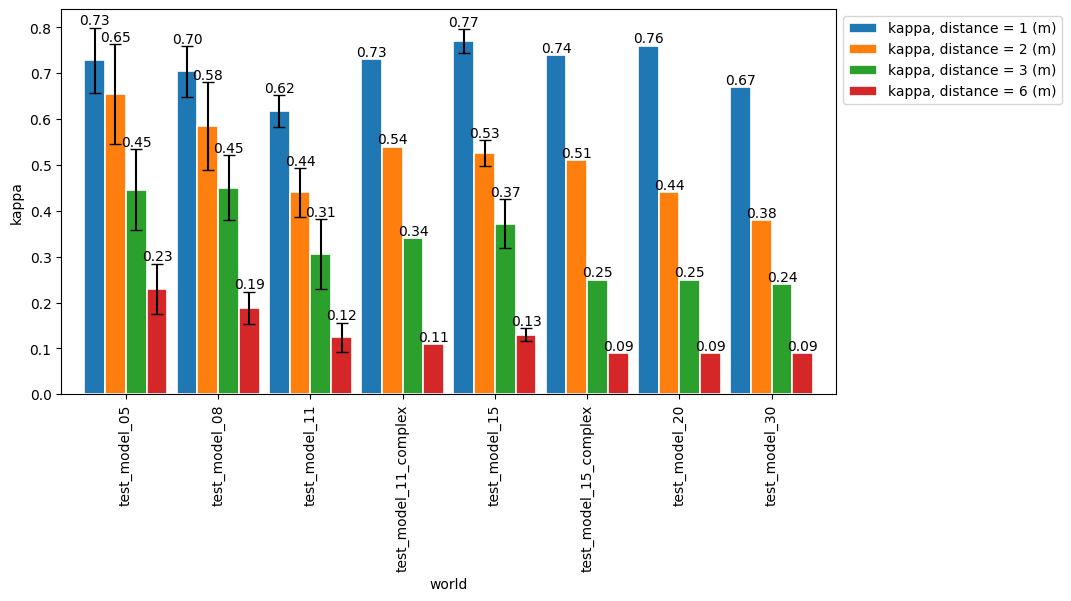
\includegraphics[width=\linewidth]{graphics/peinture_au_rouleau-kappa_vs_world_for_each_d.png}
					\caption{$\kappa$ en fonction de la densité du monde}
					\label{fig:peinture_au_rouleau-kappa_vs_world}
				\end{subfigure}
				\hfill
				\begin{subfigure}[t]{0.9\linewidth}
						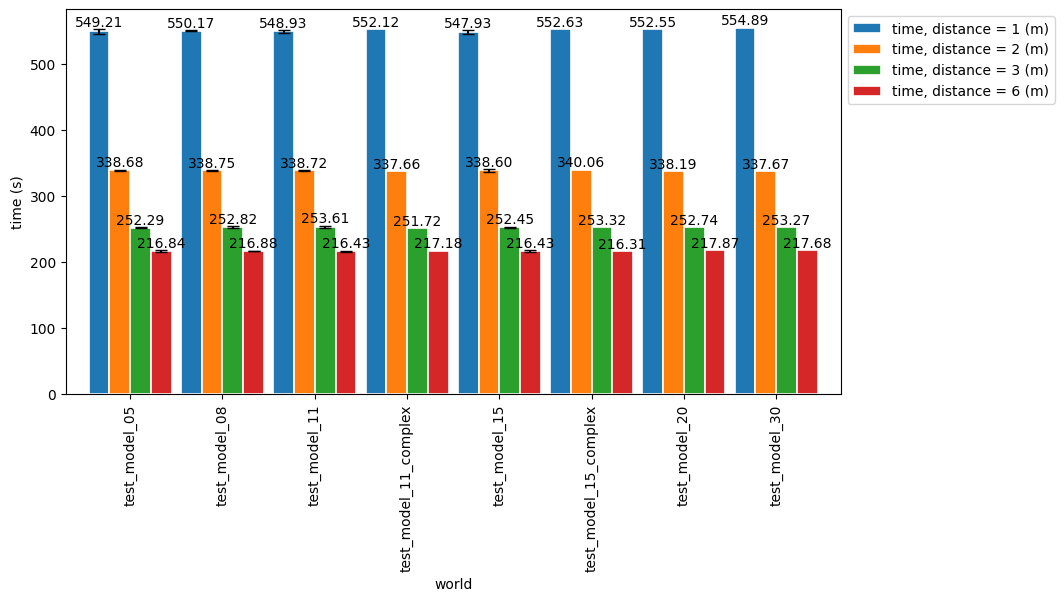
\includegraphics[width=\linewidth]{graphics/peinture_au_rouleau-time_vs_world_for_each_d.png}
						\caption{Temps d'exécution en fonction de la densité du monde}
						\label{fig:peinture_au_rouleau-time_vs_world}
				\end{subfigure}
				\caption{Évolution du $\kappa$ de Cohen et du temps d'exécution de l'algorithme \textit{peinture au rouleau} en fonction de la densité du monde et de la distance entre les robots.}
				\label{fig:peinture_au_rouleau-world}
			\end{figure}

			Premièrement, nous pouvons observer que le score de Cohen diminue, de manière générale, avec le nombre de zones de corrosion.
			Il existe des exceptions, notamment pour la carte composée de 15 zones de corrosion, où le score de Cohen est plus élevé que pour les cartes composées de 5, 8 et 11 zones de corrosion.
			Cela s'explique du fait que dans les cartes composées de 5, 8 et 11 zones de corrosion, nous avons introduit des zones de corrosion de formes allongées contrairement à la carte composée de 15 zones de corrosion où les zones de corrosion sont toutes des cercles.
			En effet, les zones de corrosion de formes allongées ont une probabilité plus grande de faire apparaître des zones fantômes, illustrées sur la figure~\ref{fig:ghost_zone}, que les zones de corrosion de forme circulaire.
			Ces zones fantômes sont des zones libres de corrosion qui sont détectées par les crawlers.
			Il s'agit donc de faux positifs qui diminuent le score de Cohen.
			Ces zones fantômes ont également plus de chance d'apparaître lorsque la densité du monde est élevée et que, donc, les zones de corrosion sont plus proches les unes des autres, ou encore lorsque la distance $d$ entre les deux crawlers est élevée.
			C'est bien ce que nous pouvons observer sur la figure~\ref{fig:peinture_au_rouleau-kappa_vs_distance} où le score de Cohen diminue lorsque la distance $d$ entre les deux crawlers augmente.
			Nous observons qu'il semble exister une relation linéaire entre le score de Cohen et la distance $d$ entre les deux crawlers.

			\begin{figure}[h!]
				\begin{subfigure}[t]{0.49\linewidth}
					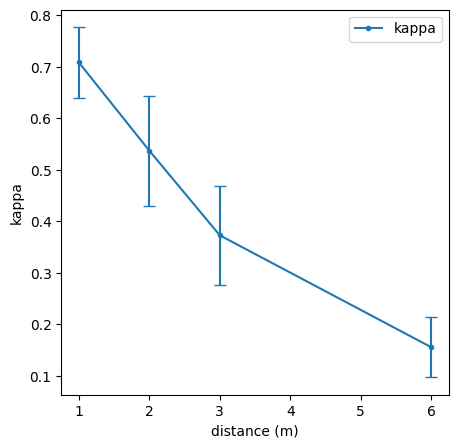
\includegraphics[width=\linewidth]{graphics/peinture_au_rouleau-kappa_vs_distance.png}
					\caption{$\kappa$ en fonction de la distance entre les deux crawlers}
					\label{fig:peinture_au_rouleau-kappa_vs_distance}
				\end{subfigure}
				\hfill
				\begin{subfigure}[t]{0.49\linewidth}
						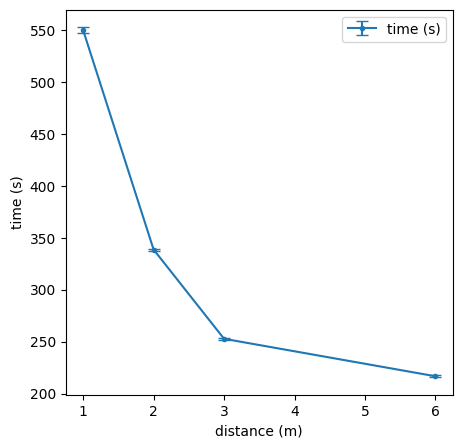
\includegraphics[width=\linewidth]{graphics/peinture_au_rouleau-time_vs_distance.png}
						\caption{Temps d'exécution en fonction de la distance entre les deux crawlers}
						\label{fig:peinture_au_rouleau-time_vs_distance}
				\end{subfigure}
				\caption{Évolution du $\kappa$ de Cohen et du temps d'exécution de l'algorithme \textit{peinture au rouleau} en fonction de la distance qui sépare les deux crawlers.}
				\label{fig:peinture_au_rouleau-distance}
			\end{figure}

			\begin{figure}[h!]
				\centering
				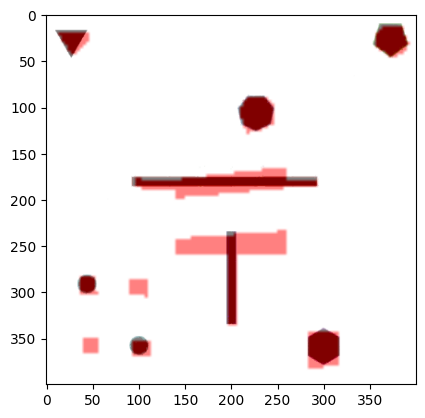
\includegraphics[width=0.5\linewidth]{graphics/output.png}
				\caption{Exemple de zone fantôme situé en bas à gauche de la carte.}
				\label{fig:ghost_zone}
			\end{figure}

			Ensuite, nous observons que le temps d'exécution de l'algorithme \textit{peinture au rouleau} est constant pour chaque valeur du nombre de zones de corrosion.
			Cela était attendu du fait que l'algorithme en question est un algorithme \textit{a priori} et ne dépend donc pas du nombre de zones de corrosion.
			En revanche, le temps d'exécution dépend de la distance $d$ entre les deux crawlers.
			Comme nous pouvons observer sur la figure~\ref{fig:peinture_au_rouleau-time_vs_distance}, le temps d'exécution augmente lorsque la distance $d$ entre les deux crawlers diminue.
			Cela s'explique du fait que plus la distance $d$ est grande, moins les crawlers doivent effectuer de déplacements pour couvrir la carte.
			Il ne semble pas exister de relation linéaire entre le temps d'exécution et la distance $d$ entre les deux crawlers.
			Or, nous nous serions attendus à ce qu'il existe une relation linéaire entre le temps d'exécution et la distance $d$ entre les deux crawlers.
			Il serait intéressant de vérifier s'il n'y a pas eu de biais introduit lors de l'implémentation de l'algorithme.

			Nous avons également introduit deux cartes avec des formes plus complexes que les cartes de base.
			Celles-ci sont visibles en annexe~\ref{annexe:cartes}, sur les figures~\ref{fig:test_model_11_complex_1} et~\ref{fig:test_model_15_complex_1}.
			Malheureusement, nous n'avons pas pu, par soucis de temps, faire varier la position des zones de corrosion, comme nous l'avons fait avec les cartes de faible densité.
			Néanmoins, il semble ne pas exister de différence significative entre les cartes de formes complexes et les cartes de formes simples.
			Par exemple, pour les cartes avec 15 formes de corrosion et la carte avec 15 formes de corrosion complexes, le score de Cohen ne varie que de 0.02 en moyenne pour une distance $d = 1$ et de 0.04 en moyenne pour une distance $d = 6$.

			Dans la suite de ce rapport, nous considérerons une distance $d = 3$ mètres entre les deux crawlers pour l'algorithme \textit{peinture au rouleau}.
		\subsection*{Stratégie de navigation \textit{ski nordique}}
			Nous allons maintenant analyser les résultats obtenus pour l'algorithme \textit{ski nordique}.
			Comme pour l'algorithme \textit{peinture au rouleau}, nous avons fait varier la densité du monde et la distance $d$ entre les deux crawlers, mais également le pas $s$ utilisé entre les deux crawlers.
			La figure~\ref{fig:ski_nordique-world_d} présente l'évolution du score de Cohen et du temps d'exécution de l'algorithme \textit{ski nordique} en fonction de la densité du monde pour différentes valeurs de la distance $d$ entre les deux crawlers et un pas $s = 3$ mètres.

			\begin{figure}[h!]
				\centering
				\begin{subfigure}[t]{0.9\linewidth}
					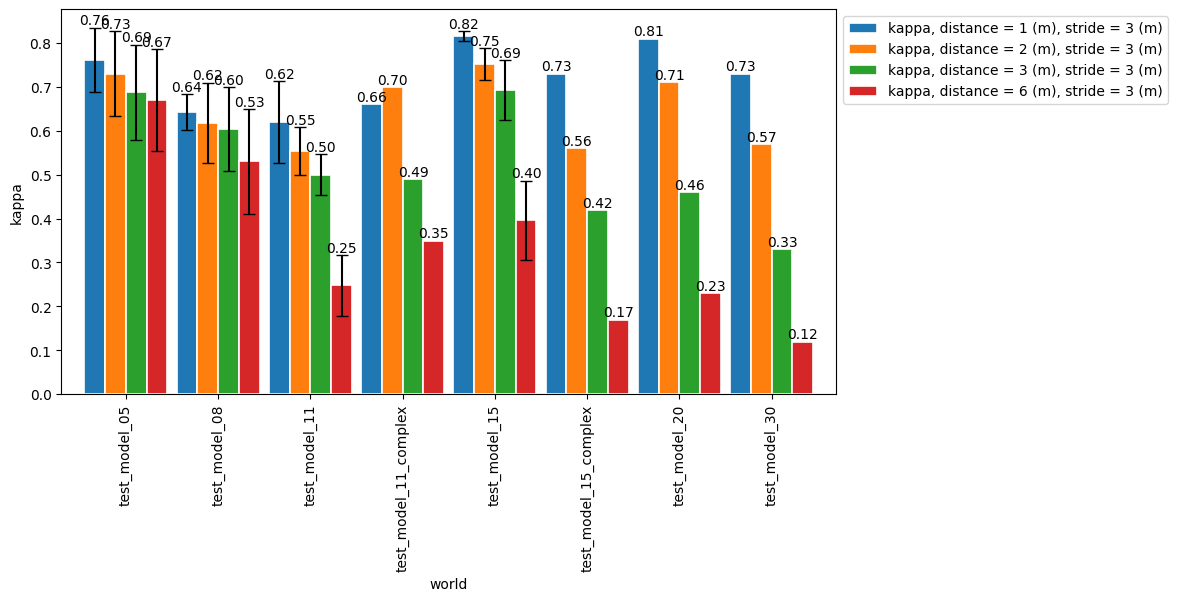
\includegraphics[width=\linewidth]{graphics/ski_nordique-kappa_vs_world_for_each_d.png}
					\caption{$\kappa$ en fonction de la densité du monde}
					\label{fig:ski_nordique-kappa_vs_world_d}
				\end{subfigure}
				\hfill
				\begin{subfigure}[t]{0.9\linewidth}
						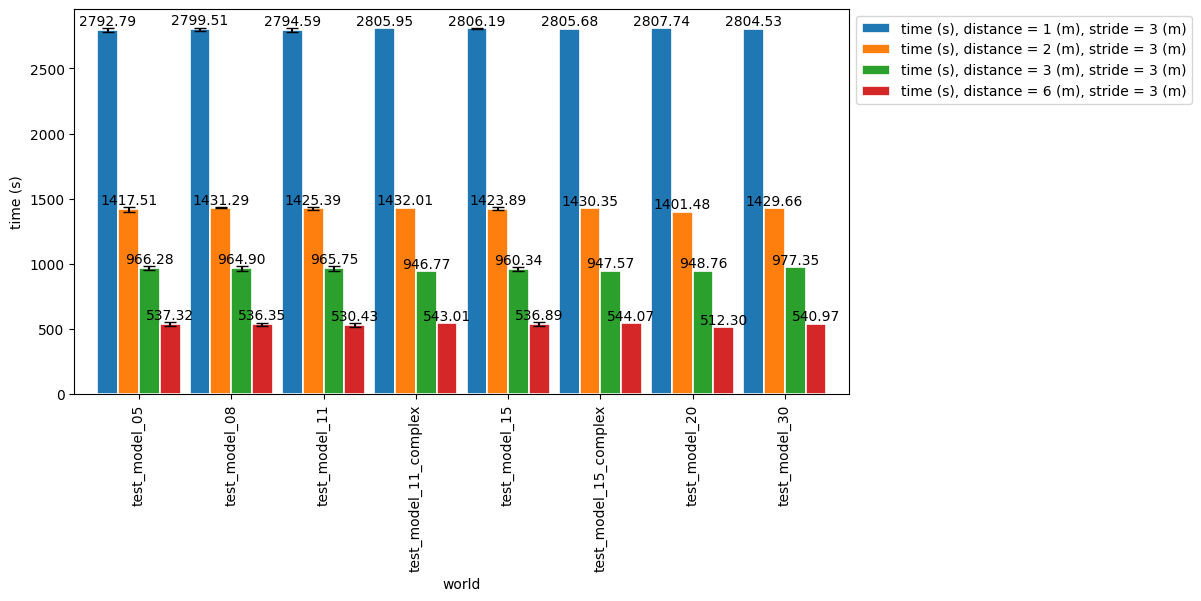
\includegraphics[width=\linewidth]{graphics/ski_nordique-time_vs_world_for_each_d.png}
						\caption{Temps d'exécution en fonction de la densité du monde}
						\label{fig:ski_nordique-time_vs_world_d}
				\end{subfigure}
				\caption{Évolution du $\kappa$ de Cohen et du temps d'exécution de l'algorithme \textit{ski nordique} en fonction de la densité du monde pour différentes valeurs de la distance entre les deux crawlers.}
				\label{fig:ski_nordique-world_d}
			\end{figure}

			Nous avons des résultats très similaires à ceux obtenus pour l'algorithme \textit{peinture au rouleau}.
			En effet, nous observons sur la figure~\ref{fig:ski_nordique-kappa_vs_world_d} que le score de Cohen diminue de manière générale lorsque la densité du monde augmente.
			De plus, le temps d'exécution de l'algorithme \textit{ski nordique}, observé sur la figure~\ref{fig:ski_nordique-time_vs_world_d}, est constant pour chaque valeur de la densité du monde.

			\begin{figure}[h!]
				\centering
				\begin{subfigure}[t]{0.9\linewidth}
					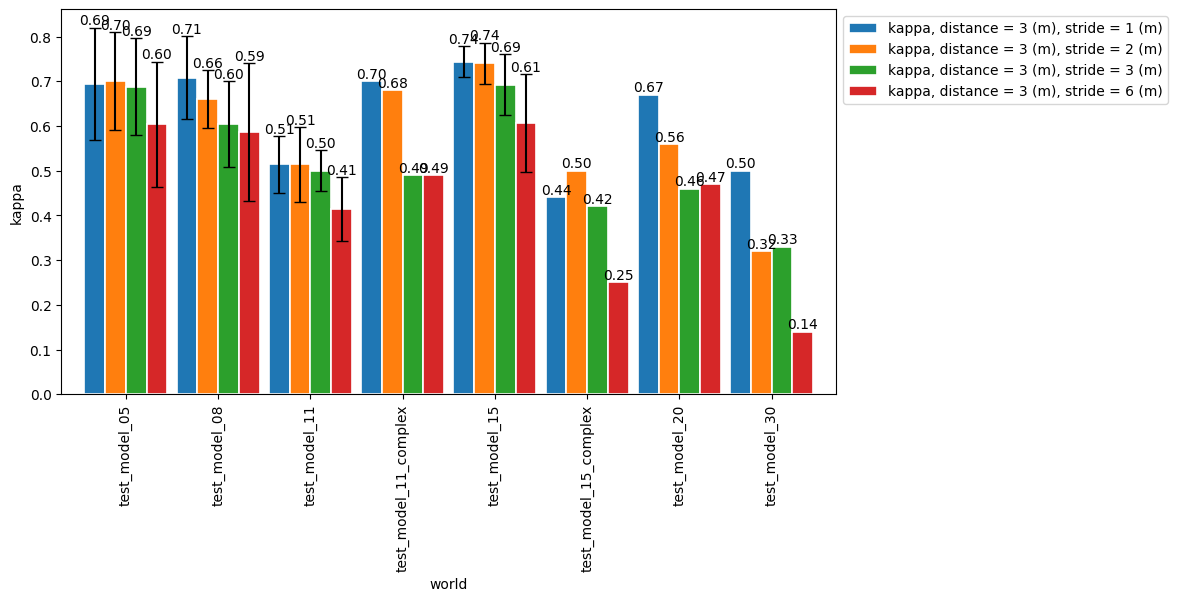
\includegraphics[width=\linewidth]{graphics/ski_nordique-kappa_vs_world_for_each_s.png}
					\caption{$\kappa$ en fonction de la densité du monde}
					\label{fig:ski_nordique-kappa_vs_world_s}
				\end{subfigure}
				\hfill
				\begin{subfigure}[t]{0.9\linewidth}
						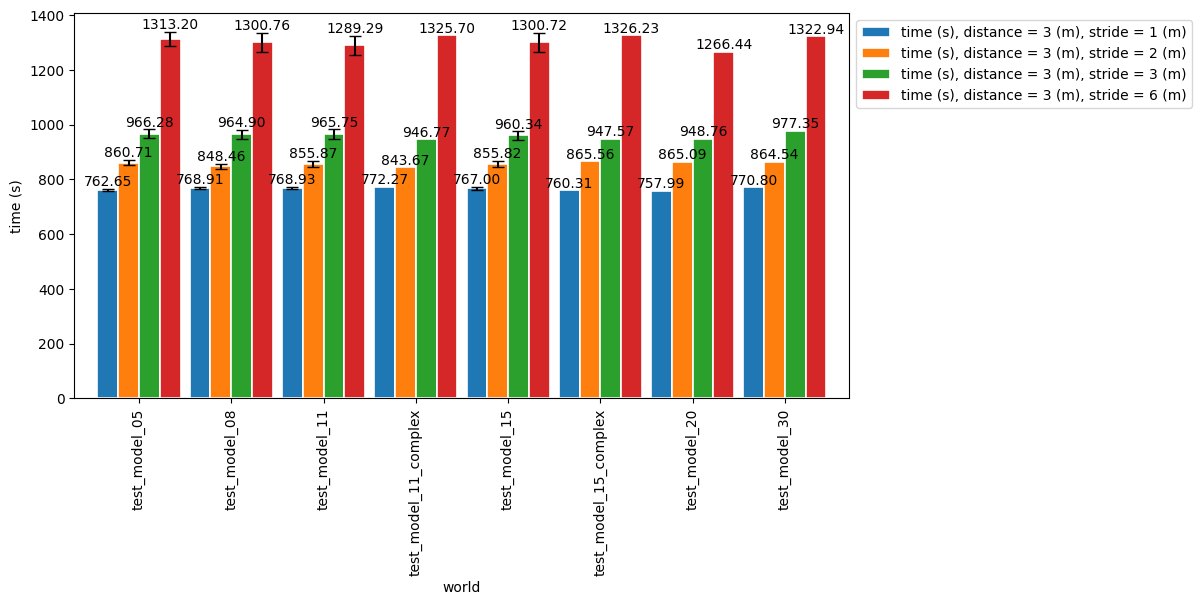
\includegraphics[width=\linewidth]{graphics/ski_nordique-time_vs_world_for_each_s.png}
						\caption{Temps d'exécution en fonction de la densité du monde}
						\label{fig:ski_nordique-time_vs_world_s}
				\end{subfigure}
				\caption{Évolution du $\kappa$ de Cohen et du temps d'exécution de l'algorithme \textit{ski nordique} en fonction de la densité du monde pour différentes valeurs du pas entre les deux crawlers.}
				\label{fig:ski_nordique-world_s}
			\end{figure}

			Nous pouvons observer sur la figure~\ref{fig:ski_nordique-world_s} l'évolution du score de Cohen et du temps d'exécution de l'algorithme \textit{ski nordique} en fonction de la densité du monde pour différentes valeurs du pas $s$ entre les deux crawlers, et une distance $d = 3$ mètres entre les crawlers.
			sur la figure~\ref{fig:ski_nordique-kappa_vs_world_s}, nous observons que le score de Cohen est le plus bas pour de grandes valeurs de densités et de grandes valeurs de $d$, comme pour $d = 6$ mètres et les cartes avec 30 et 20 zones de corrosion.
			Ceci s'explique par le fait que pour de grandes valeurs de densités et de $d$, la probabilité que les rayons du signal traversent des zones de corrosions est plus élevée.
			Il y a donc plus de chance que des zones fantômes soient créées, ce qui fait diminuer le score de Cohen.
			Les formes allongées des zones de corrosion sont également un facteur qui fait diminuer le score de Cohen comme étudié précédemment.
			C'est pourquoi nous observons que le score de Cohen est le plus haut pour la carte avec la plus petite densité et sans formes allongées de corrosion, c'est-à-dire la carte avec 15 zones de corrosion.

			Sur la figure~\ref{fig:ski_nordique-time_vs_world_s}, nous observons que le temps d'exécution de l'algorithme \textit{ski nordique} est constant pour chaque valeur de la densité du monde.
			Ceci était attendu comme pour la stratégie \textit{peinture au rouleau}.
			Cependant, nous observons que le temps d'exécution varie avec le pas $s$ utilisé.
			Nous nous serions plutôt attendus à ce que le temps d'exécution reste constant avec le pas des crawlers.
			En effet, indépendamment de la valeur du pas, la distance verticale et horizontale à parcourir par les crawlers reste la même.
			Cette différence significative du temps d'exécution est due à la manière dont nous avons implémenté l'algorithme \textit{ski nordique} qui n'est pas optimale.
			Nous n'avons pas fait arrêter les crawlers aux extrémités des plaques, mais nous les avons fait continuer d'une valeur du pas $s$, en plus, par simplicité d'implémentation sans penser que l'impact sur le temps d'exécution serait significatif.

			\begin{figure}[h!]
				\begin{subfigure}[t]{0.49\linewidth}
					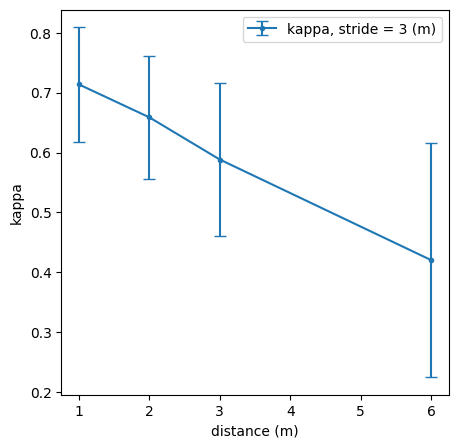
\includegraphics[width=\linewidth]{graphics/ski_nordique-kappa_vs_distance.png}
					\caption{$\kappa$ en fonction de la distance entre les deux crawlers}
					\label{fig:ski_nordique-kappa_vs_distance}
				\end{subfigure}
				\hfill
				\begin{subfigure}[t]{0.49\linewidth}
						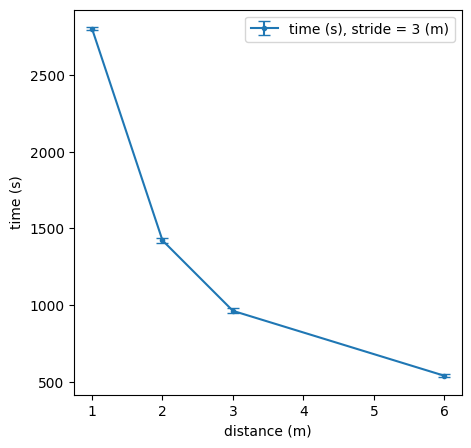
\includegraphics[width=\linewidth]{graphics/ski_nordique-time_vs_distance.png}
						\caption{Temps d'exécution en fonction de la distance entre les deux crawlers}
						\label{fig:ski_nordique-time_vs_distance}
				\end{subfigure}
				\caption{Évolution du $\kappa$ de Cohen et du temps d'exécution de l'algorithme \textit{ski nordique} en fonction de la distance qui sépare les deux crawlers.}
				\label{fig:ski_nordique-distance}
			\end{figure}

			Sur la figure~\ref{fig:ski_nordique-distance}, nous observons l'évolution du score de Cohen et du temps d'exécution de l'algorithme \textit{ski nordique} en fonction de la distance qui sépare les deux crawlers pour un pas de 3 mètres.
			Le score semble, comme pour la stratégie \textit{peinture au rouleau}, suivre une relation linéaire avec la distance qui sépare les deux crawlers.
			Le temps d'exécution semble également suivre une relation linéaire avec la distance qui sépare les deux crawlers.
			Le fait que la courbe à figure~\ref{fig:ski_nordique-time_vs_distance} ne soit pas une droite est dû au fait que plus la distance entre les crawlers est petite et plus le nombre de rotations que les crawlers doivent effectuer est grand.
			Or le temps de rotation n'est pas négligeable dans les temps d'exécution des algorithmes.

			\begin{figure}[h!]
				\begin{subfigure}[t]{0.49\linewidth}
					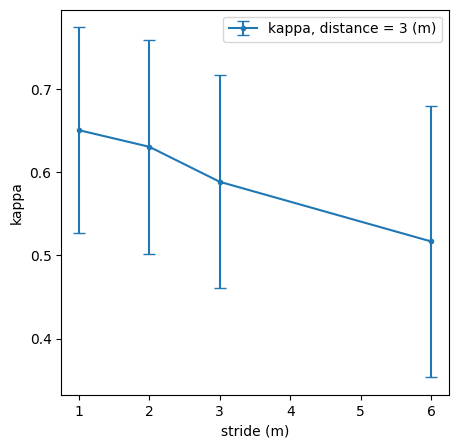
\includegraphics[width=\linewidth]{graphics/ski_nordique-kappa_vs_stride.png}
					\caption{$\kappa$ en fonction du pas des crawlers}
					\label{fig:ski_nordique-kappa_vs_stride}
				\end{subfigure}
				\hfill
				\begin{subfigure}[t]{0.49\linewidth}
						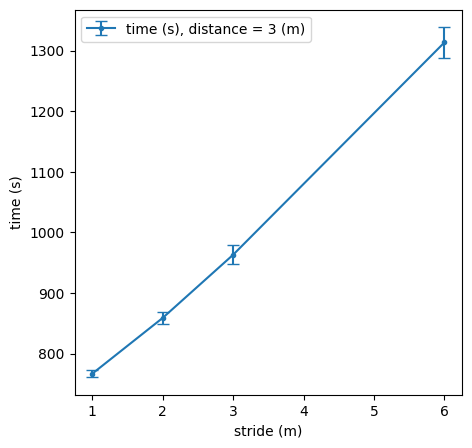
\includegraphics[width=\linewidth]{graphics/ski_nordique-time_vs_stride.png}
						\caption{Temps d'exécution en fonction du pas des crawlers}
						\label{fig:ski_nordique-time_vs_stride}
				\end{subfigure}
				\caption{Évolution du $\kappa$ de Cohen et du temps d'exécution de l'algorithme \textit{ski nordique} en fonction du pas des crawlers.}
				\label{fig:ski_nordique-stride}
			\end{figure}

			Sur la figure~\ref{fig:ski_nordique-stride}, nous observons l'évolution du score de Cohen et du temps d'exécution de l'algorithme \textit{ski nordique} en fonction du pas $s$ des crawlers pour une distance $d = 3$ mètres.
			Le score semble suivre une relation linéaire avec le pas des crawlers.
			Plus le pas est petit et plus le score est grand.
			Cela entre en concordance avec ce que nous expliquions précédemment.
			Plus le pas est grand et plus, il y a de chance de créer des zones fantômes et donc, de faire diminuer le score de Cohen.
			Il est a noté cependant qu'il existe une grande variation du score pour les différentes valeurs du pas.
			Il semble donc que l'impact de la valeur du pas sur le score soit plutôt faible contrairement à l'impact de la valeur de la distance sur le score.
			Le temps d'exécution, lui, semble suivre une relation linéaire avec le pas des crawlers.
			Comme expliqué précédemment, ce dernier aurait dû être constant, mais notre implémentation fait dépendre le temps d'exécution du pas des crawlers.

			Ici encore, il semble que le score et le temps d'exécution ne soient pas affectés par le fait que les formes soient complexes ou non.

			Dans la suite de ce rapport, nous considérerons une distance $d = 3$ entre les deux crawlers et un pas $s = 3$ pour l'algorithme \textit{ski nordique}.
		\subsection*{Stratégie de navigation \textit{investigation polygonale}}
			Nous avons ensuite testé l'algorithme \textit{investigation polygonale} sur des mondes composés de 5, 8 et 11 zones de corrosion.
			La stratégie d'inspection se base sur les résultats de la stratégie \textit{peinture au rouleau}.
			Comme expliqué précédemment, nous justifions ce choix par le fait que la stratégie \textit{peinture au rouleau} est la plus rapide des stratégies \textit{a priori} que nous avons implémenté.

			\begin{figure}[h!]
				\begin{subfigure}[t]{0.9\linewidth}
					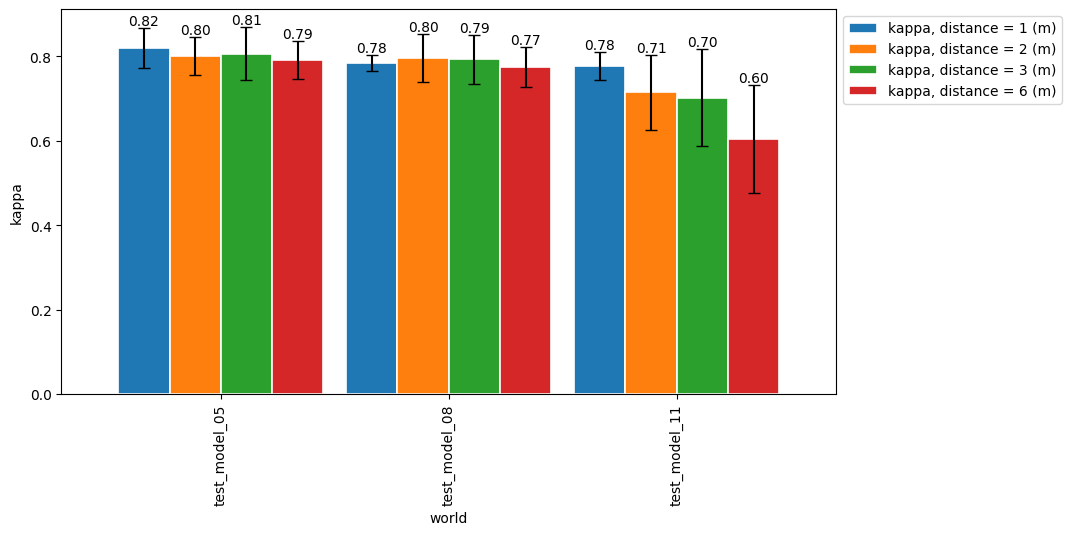
\includegraphics[width=\linewidth]{graphics/investigation_polygonale-kappa_vs_world_for_each_d_k1_n2_p4.png}
					\caption{$\kappa$ en fonction de la densité du monde}
					\label{fig:investigation_polygonale-kappa_vs_world_for_each_d_k1_n2_p4}
				\end{subfigure}
				\hfill
				\begin{subfigure}[t]{0.9\linewidth}
						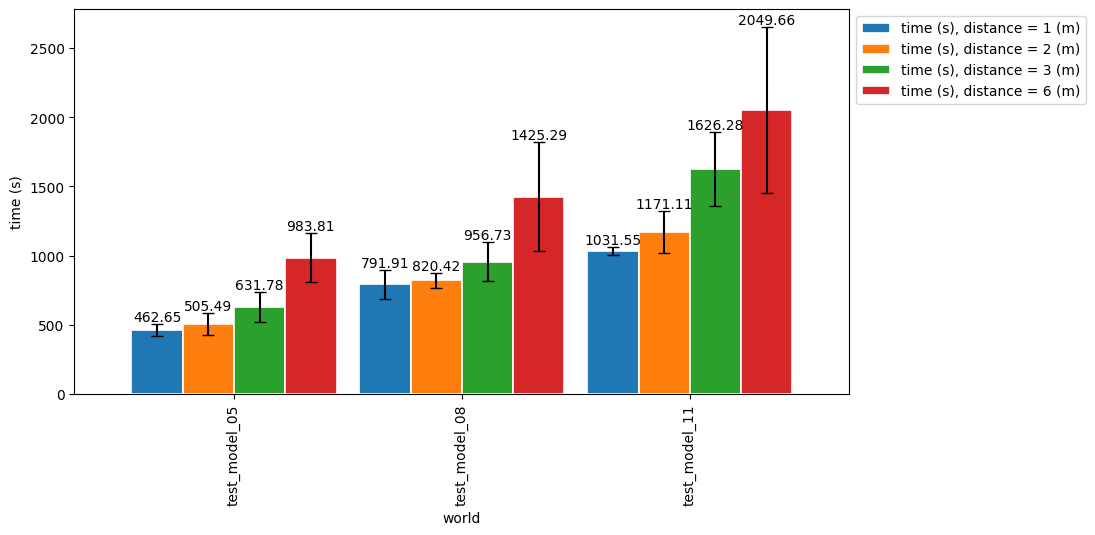
\includegraphics[width=\linewidth]{graphics/investigation_polygonale-time_vs_world_for_each_d_k1_n2_p4.png}
						\caption{Temps d'exécution en fonction de la densité du monde}
						\label{fig:investigation_polygonale-time_vs_world_for_each_d_k1_n2_p4}
				\end{subfigure}
				\caption{Évolution du $\kappa$ de Cohen et du temps d'exécution de l'algorithme \textit{investigation polygonale} en fonction de la densité du monde pour différentes distances entre les crawlers avec un polygone à 4 côtés.}
				\label{fig:investigation_polygonale-world_for_each_d_k1_n2_p4}
			\end{figure}

			La figure~\ref{fig:investigation_polygonale-kappa_vs_world_for_each_d_k1_n2_p4} montre l'évolution du score de Cohen en fonction de la densité du monde pour chaque valeur de $d$ utilisée dans la stratégie \textit{peinture au rouleau}.
			Nous avons utilisé un polygone d'investigation à 4 côtés.
			En premier lieu, nous observons des scores de Cohen relativement indépendant de la distance entre les crawlers pour les cartes avec 5 et 8 zones de corrosion.
			Ceci est un résultat enthousiasmant, car cela signifie que nous pouvons utiliser la stratégie \textit{investigation polygonale} en se basant sur les résultats de la stratégie \textit{peinture au rouleau} en utilisant une grande distance entre les crawlers, et donc, une stratégie \textit{peinture au rouleau} très rapide.
			Néanmoins, nous pouvons observer que pour les cartes avec 11 zones de corrosion, le score de Cohen est impacté par la distance entre les crawlers, lorsque cette dernière augmente.
			Nous imputons ce résultat au fait que cette carte comporte des zones de corrosion allongées très proches les unes des autres, ayant pour effet de bloquer certains rayons émis et reçus lors de l'inspection polygonale d'une zone.
			L'inspection polygonale est donc naturellement impactée par la densité du monde.
			Cepandant, nous pouvons imaginer, lors de la réparation des structures métalliques, qu'il soit plus convenable de fusionner des zones de corrosion proches les unes des autres en une seule zone de corrosion, bien que cela ne soit pas considéré dans notre problème.

			La figure~\ref{fig:investigation_polygonale-time_vs_world_for_each_d_k1_n2_p4} montre l'évolution du temps d'exécution en fonction de la densité du monde pour chaque valeur de $d$ utilisée dans la stratégie \textit{peinture au rouleau}.
			Nous avons utilisé un polygone d'investigation à 4 côtés.
			Nous observons que le temps d'exécution augmente avec la densité du monde de manière linéaire.
			Ceci est un résultat attendu, car l'algorithme \textit{investigation polygonale} est de complexité linéaire en fonction du nombre de zones de corrosion, ce dernier consistant à parcourir toutes les zones de corrosion potentielles et à les inspecter.
			Nous observons également que le temps d'exécution augmente avec la distance entre les crawlers.
			En effet, plus la distance entre les crawlers est grande, plus le nombre de zones fantômes est important à l'issue de la stratégie de navigation \textit{peinture au rouleau}, et donc plus le nombre de zones de corrosion potentielles est important.
			Cependant, ces zones fantômes sont rapidement traitées par l'algorithme \textit{investigation polygonale}.
			Par exemple, pour la carte 5 avec 11 zones de corrosion, nous obtenons 12 zones de corrosion potentielles avec une distance de 1 mètre entre les crawlers à l'issue de la stratégie \textit{peinture au rouleau}, contre 20 zones de corrosion potentielles avec une distance de 6 mètres entre les crawlers.
			Or, nous observons un temps d'exécution de 1027 secondes pour la première configuration contre 1616 secondes pour la seconde configuration.
			Nous avons donc pour une augmentation de 67\% du nombre de zones de corrosion potentielles, une augmentation de 57\% du temps d'exécution.
			Le gain de performance n'est pas très important, mais est tout de même significatif.

			\begin{figure}[h!]
				\begin{subfigure}[t]{0.9\linewidth}
					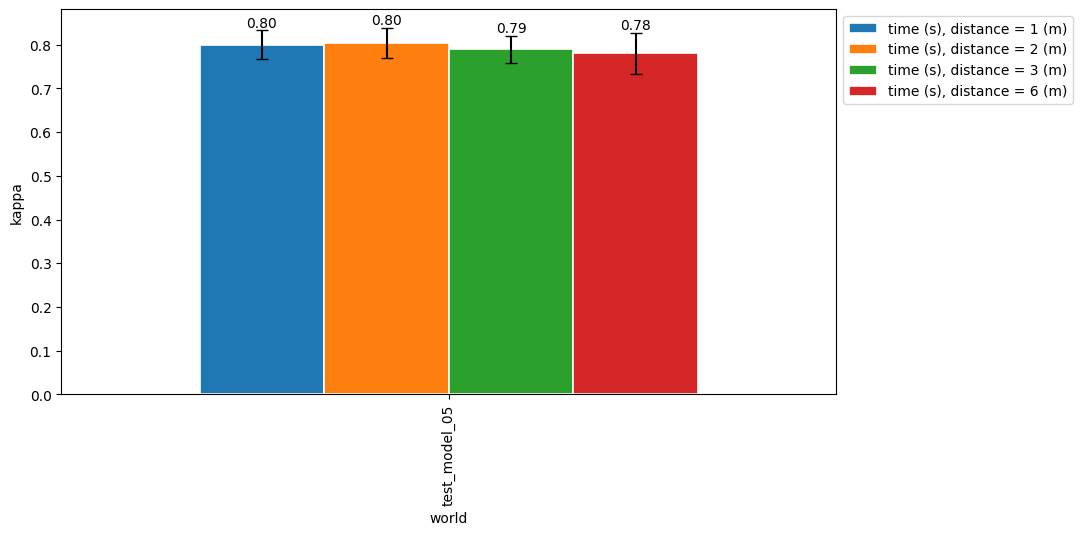
\includegraphics[width=\linewidth]{graphics/investigation_polygonale-kappa_vs_world_for_each_d_k1_n2_p6.png}
					\caption{$\kappa$ en fonction de la densité du monde}
					\label{fig:investigation_polygonale-kappa_vs_world_for_each_d_k1_n2_p6}
				\end{subfigure}
				\hfill
				\begin{subfigure}[t]{0.9\linewidth}
						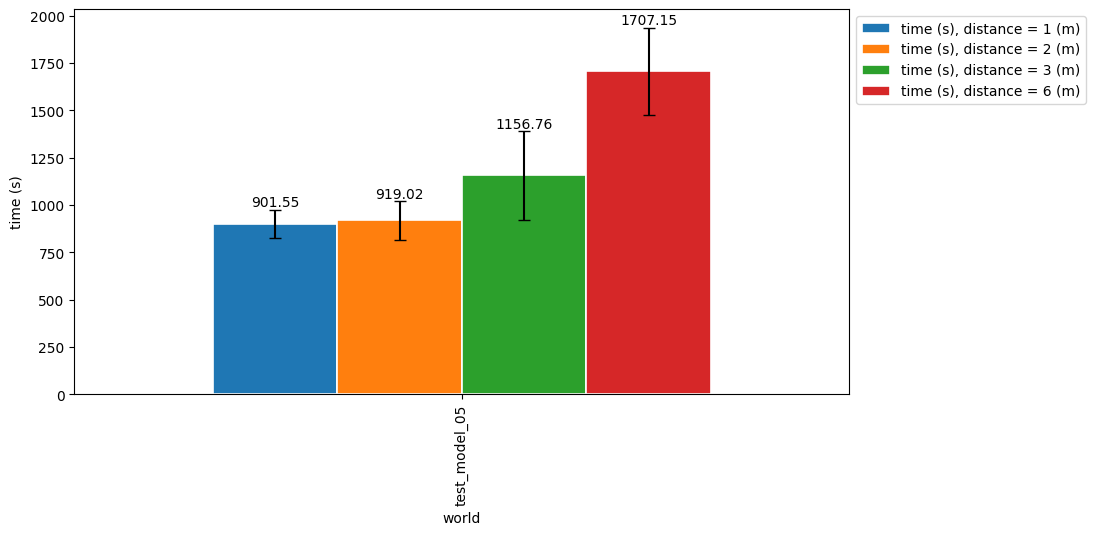
\includegraphics[width=\linewidth]{graphics/investigation_polygonale-time_vs_world_for_each_d_k1_n2_p6.png}
						\caption{Temps d'exécution en fonction de la densité du monde}
						\label{fig:investigation_polygonale-time_vs_world_for_each_d_k1_n2_p6}
				\end{subfigure}
				\caption{Évolution du $\kappa$ de Cohen et du temps d'exécution de l'algorithme \textit{investigation polygonale} en fonction de la densité du monde pour différentes distances entre les crawlers avec un polygone à 6 côtés.}
				\label{fig:investigation_polygonale-world_for_each_d_k1_n2_p6}
			\end{figure}

			Nous avons également fait varier la taille du polygone d'investigation de la stratégie \textit{investigation polygonale}.
			Nous présentons sur la figure~\ref{fig:investigation_polygonale-kappa_vs_world_for_each_d_k1_n2_p6} l'évolution du score de Cohen en fonction de la densité du monde pour la carte 5, pour un polygone à 6 sommets.
			Premièrement, nous n'observons pas une amélioration significative du score de Cohen lorsque la taille du polygone d'investigation augmente.
			Au contraire, nous observons une diminution en moyenne, bien que très faible, du score.
			En théorie, l'augmentation de la taille du polygone d'investigation devrait permettre de mieux approcher l'enveloppe convexe des zones de corrosion, et donc d'obtenir un meilleur score de Cohen.
			Cependant, nous sommes limités dans notre implémentation par la résolution utilisée pour la discrétisation de la carte.
			% Ainsi, il est probable que le fait d'augmenter la taille du polygone d'investigation élimine des cellules de la grille d'occupation (en périphérie des zones de corrosion) où de la corrosion est réellement présente, du fait qu'il ait existé un rayon qui ait traversé cette même cellule.
			Cependant, pour une résolution plus précise, nous devrions observer une amélioration du score de Cohen.

			Nous présentons sur la figure~\ref{fig:investigation_polygonale-time_vs_world_for_each_d_k1_n2_p6} l'évolution du temps d'exécution en fonction de la densité du monde pour la carte 5, pour un polygone à 6 sommets.
			Ici, nous observons naturellement une augmentation du temps d'exécution lorsque la taille du polygone d'investigation augmente.

			Nous aurions également voulu faire varier le nombre de robots utilisés pour l'investigation polygonale ainsi que le nombre d'équipes de robots.
			Cependant, nous n'avons pas eu le temps de mettre en place une solution de gestion des collisions entre les robots.
			Il serait intéressant dans un travail futur de mettre en place une telle solution et d'analyser les performances de l'algorithme \textit{investigation polygonale} avec ces différents paramètres.
			En effet, le temps d'exécution de l'algorithme \textit{investigation polygonale} devrait diminuer lorsque $k$ et $n$ augmentent.

			Dans la sous-section suivante, nous comparerons les performances de l'algorithme \textit{investigation polygonale} avec celles des algorithmes \textit{peinture au rouleau} et \textit{ski nordique}.
			Pour ce faire, nous considérerons un polygone d'investigation pour l'investigation polygonale à $p = 4$ sommets.
		\subsection*{Comparaisons et discussions}
			Dans cette sous-section, nous comparons les performances des différentes stratégies de navigation multi-robots.

			\begin{figure}[h!]
				\begin{subfigure}[t]{0.9\linewidth}
					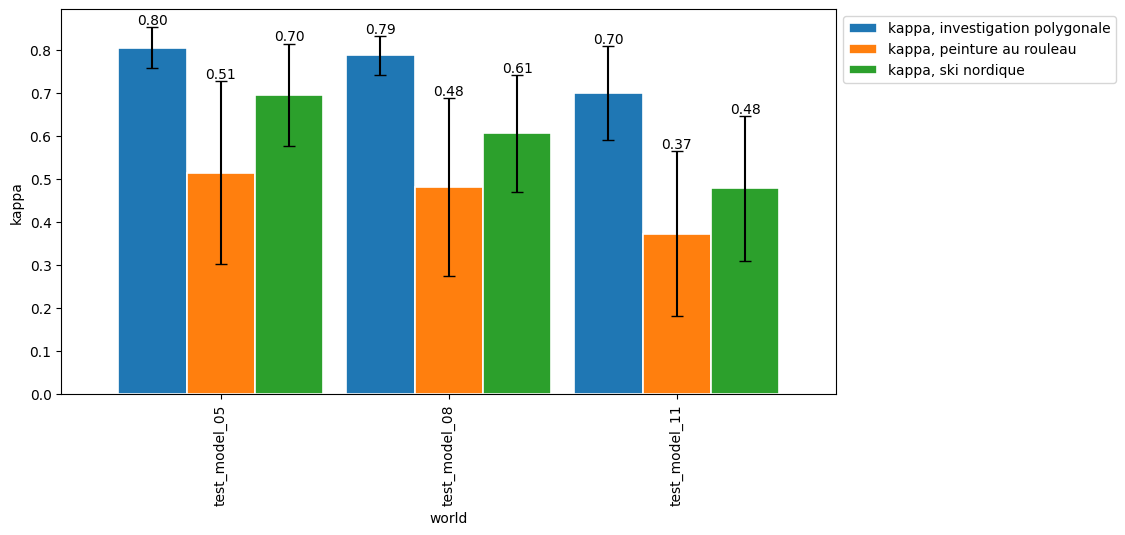
\includegraphics[width=\linewidth]{graphics/investigation_polygonale-peinture_au_rouleau_ski_nordique-kappa_for_each_world_vs_investigation_polygonale-kappa_for_each_world.png}
					\caption{$\kappa$ en fonction de la densité du monde}
					\label{fig:investigation_polygonale-peinture_au_rouleau_ski_nordique-kappa_for_each_world_vs_investigation_polygonale-kappa_for_each_d}
				\end{subfigure}
				\hfill
				\begin{subfigure}[t]{0.9\linewidth}
						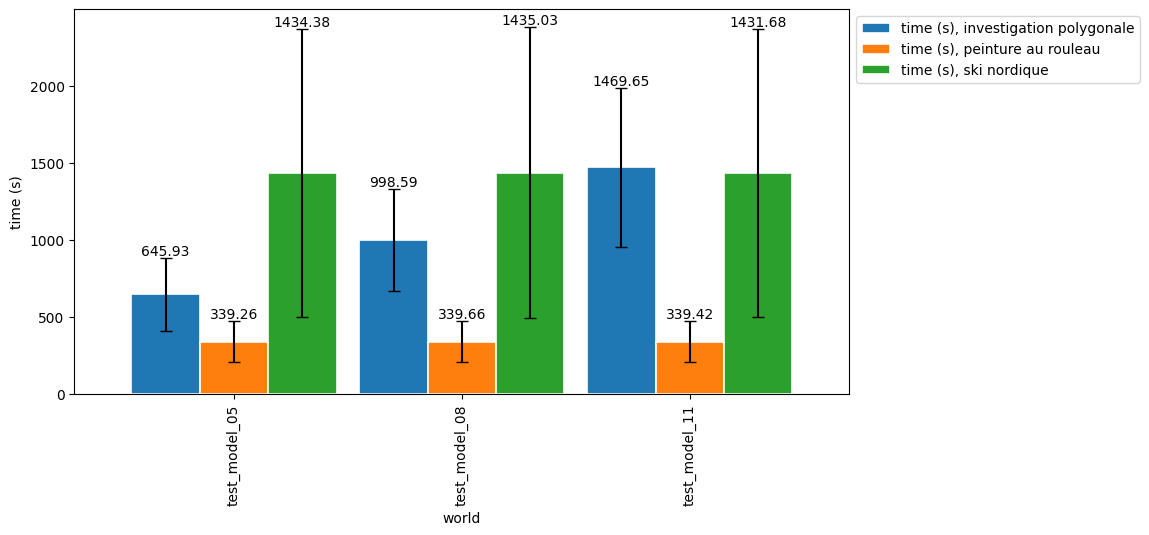
\includegraphics[width=\linewidth]{graphics/investigation_polygonale-peinture_au_rouleau_ski_nordique-time_for_each_world_vs_investigation_polygonale-time_for_each_world.png}
						\caption{Temps d'exécution en fonction de la densité du monde}
						\label{fig:investigation_polygonale-peinture_au_rouleau_ski_nordique-time_for_each_world_vs_investigation_polygonale-time_for_each_d}
				\end{subfigure}
				\caption{Évolution du $\kappa$ de Cohen et du temps d'exécution des différents algorithmes en fonction de la densité du monde pour différentes distances entre les crawlers.}
				\label{fig:investigation_polygonale-peinture_au_rouleau_ski_nordique_for_each_world}
			\end{figure}

			Nous présentons sur la figure~\ref{fig:investigation_polygonale-peinture_au_rouleau_ski_nordique_for_each_world} l'évolution du score de Cohen et du temps d'exécution en fonction de la densité du monde, pour chaque algorithme.
			Dans cette figure, nous avons représenté les scores et temps d'exécution obtenus, en moyenne, pour les différentes valeurs de $d$ et de $s$, par soucis de lisibilité.
			Une version plus détaillée, pour chaque valeur de $d$, est disponible en annexe~\ref{annexe:comparaison}, sur la figure~\ref{fig:investigation_polygonale-peinture_au_rouleau_ski_nordique_for_each_d}.

			Nous pouvons observer sur la figure~\ref{fig:investigation_polygonale-peinture_au_rouleau_ski_nordique-kappa_for_each_world_vs_investigation_polygonale-kappa_for_each_d} que le score de Cohen obtenu par l'algorithme \textit{investigation polygonale} est supérieur à ceux obtenus par les algorithmes \textit{peinture au rouleau} et \textit{ski nordique}.
			Seule la stratégie \textit{investigation polygonale} a permis d'obtenir un score de Cohen considéré comme \textit{accord presque parfait} (supérieur à 0.8) selon Landis et Koch.

			Nous pouvons observer sur la figure~\ref{fig:investigation_polygonale-peinture_au_rouleau_ski_nordique-time_for_each_world_vs_investigation_polygonale-time_for_each_d} que le temps d'exécution de l'algorithme \textit{peinture au rouleau} est inférieur à ceux obtenus par les algorithmes \textit{investigation polygonale} et \textit{ski nordique}.
			Pour de faibles densités de cartes comme celles utilisées dans nos expérimentations, l'algorithme \textit{ski nordique} est le moins rapide.
			Ce résultat est à nuancer.
			En effet, pour des densités plus élevées, l'algorithme \textit{investigation polygonale} devient plus lent que l'algorithme \textit{ski nordique}, comme nous pouvons déjà presque le voir pour la carte comportant 11 zones de corrosion.

			\begin{table}[h!]
				\centering
				\begin{tabular}{|c|c|c|}
					\hline
					& \multicolumn{2}{c|}{\textbf{Gain en performance \textit{investigation polygonale}}} \\
					\hline
					\textbf{comparé à} & \textbf{$\kappa$ de Cohen} & \textbf{Temps d'exécution} \\
					\hline
					\textit{peinture au rouleau} & +68.39\% & +305.80\% \\
					\hline
					\textit{ski nordique} & +27.92\% & -3.92\% \\
					\hline
				\end{tabular}
				\caption{Gain en performance apporté par la stratégie \textit{investigation polygonale} par rapport aux stratégies \textit{peinture au rouleau} et \textit{ski nordique}.}
				\label{tab:gain}
			\end{table}

			La table~\ref{tab:gain} présente le gain en performance apporté par la stratégie \textit{investigation polygonale} par rapport aux stratégies \textit{peinture au rouleau} et \textit{ski nordique}.
			Ici, nous avons considéré le temps d'investigation de la stratégie \textit{investigation polygonale} comme étant égal à la somme des temps d'investigation de la stratégie \textit{investigation polygonale} et de la stratégie \textit{peinture au rouleau} puisque la première stratégie se base sur la seconde pour explorer les zones de corrosion.
			Nous pouvons observer que l'algorithme \textit{investigation polygonale} permet d'obtenir un score de Cohen supérieur de 68.39\% à celui obtenu par l'algorithme \textit{peinture au rouleau}, bien qu'il soit bien plus lent que ce dernier.
			En revanche, l'algorithme \textit{investigation polygonale} permet d'obtenir un score de Cohen supérieur de 27.92\% à celui obtenu par l'algorithme \textit{ski nordique}, tout en étant plus rapide que ce dernier.
	\section{Bilan personnel}
		Au cours de cette période de travail, j'ai pu approfondir mes connaissances dans le domaine de la robotique et de l'inspection multi-robots.
		J'ai été confronté à divers défis que j'ai essayé de surmonter.
		Ce projet m'a permis d'acquérir de nouvelles compétences techniques et d'améliorer ma capacité à travailler au sein d'un projet de recherche.

		Tout d'abord, j'ai pu approfondir mes connaissances en robotique et dans l'inspection multi-robots.
		J'ai effectué des recherches approfondies et j'ai consulté des sources fiables pour obtenir des informations pertinentes.
		Cela m'a permis de comprendre en profondeur les concepts clés liés à mon sujet d'étude.

		Au cours de ce projet, j'ai pu grandement évoluer sur le plan personnel et professionnel.
		J'ai acquis de nouvelles compétences et enrichi mon bagage technique, ce qui a renforcé ma confiance dans mes capacités en tant qu'ingénieur.

		Tout d'abord, j'ai considérablement développé mes compétences en programmation, en mettant l'accent sur Python et C++.
		Grâce à cette expérience, j'ai acquis une meilleure compréhension de ces langages et j'ai gagné en efficacité dans la résolution de problèmes.

		Parallèlement, j'ai eu l'opportunité d'explorer de nouveaux outils qui se sont révélés essentiels pour la réalisation de mon projet.
		J'ai notamment travaillé avec Gazebo, une plateforme de simulation d'environnements virtuels, ce qui m'a permis de tester et de valider mes algorithmes dans des conditions proches de la réalité.
		J'ai également utilisé Blender pour créer des modèles 3D. De plus, l'apprentissage de ROS (Robot Operating System) m'a offert une infrastructure logicielle solide pour le développement et le contrôle de robots.

		En outre, ma participation à ce projet m'a offert une première immersion dans le monde de la recherche.
		J'ai eu l'occasion d'explorer la littérature scientifique, de me familiariser avec les travaux antérieurs liés à mon domaine d'étude et de mettre en pratique des méthodologies de recherche.
		J'ai appris à collecter et à analyser des données, rédiger des rapports techniques, et lire des articles scientifiques.
		Cette expérience m'a permis de développer ma rigueur scientifique et ma capacité à mener des investigations approfondies.

		Enfin, ce projet m'a également permis de renforcer ma gestion du temps et de prioriser efficacement les tâches.
		J'ai dû établir un planning détaillé pour respecter les échéances et m'assurer que chaque étape du projet était réalisée en temps voulu.
		J'ai appris à gérer les imprévus et à ajuster mon emploi du temps en conséquence pour maintenir un bon équilibre entre la qualité du travail et le respect des délais.

		Dans l'ensemble, ce projet a été une expérience enrichissante qui m'a permis de développer mes compétences et de progresser dans mon domaine.
		J'ai acquis une compréhension approfondie de la robotique et de l'inspection multi-robots, renforcé mes compétences techniques et amélioré ma capacité à m'organiser.
		Je suis reconnaissant d'avoir eu l'opportunité de m'investir dans ce projet et je suis convaincu que les compétences que j'ai acquises me seront utiles dans mes futurs projets professionnels.

		En conclusion, ce projet a été une étape essentielle dans mon parcours professionnel.
		J'ai acquis des compétences techniques avancées, j'ai exploré de nouveaux outils et j'ai pu me familiariser avec les exigences de la recherche.
		Ces acquis me seront précieux pour mes projets futurs, qu'il s'agisse de poursuivre dans le domaine de la recherche ou dans l'industrie.
	\section{Conclusion et perspectives}
		En conclusion, cette étude a permis de mettre en œuvre et d'évaluer trois stratégies pour la réalisation d'une exploration muli-robots autonome dans des environnements complexes.
		Les résultats obtenus démontrent l'efficacité de ces approches dans la résolution du problème d'inspection de surfaces métalliques et mettent en évidence leurs caractéristiques respectives.

		La première stratégie, la stratégie \textit{peinture au rouleau}, a permis d'obtenir des résultats satisfaisants en des temps d'exploration très courts.
		La distance entre les robots peut être ajustée pour optimiser les résultats dépendamment de la densité des zones de corrosion inférées.
		Cette stratégie est particulièrement adaptée à une utilisation préalable à la stratégie \textit{investigation polygonale}, car elle permet de rapidement avoir une vue grossière des zones de corrosion potentielles.

		La deuxième stratégie, la stratégie \textit{ski nordique}, a permis d'obtenir des résultats supérieurs à ceux de la stratégie \textit{peinture au rouleau}, mais avec des temps d'exploration plus longs.
		Cette approche est plus robuste que la stratégie de peinture au rouleau, car elle fait varier l'orientation des rayons UGW émis et reçus, permettant ainsi de plus finement approcher les zones de corrosion.

		Enfin, la troisième stratégie, la startégie \textit{investigation polygonale}, a permis d'obtenir les meilleurs résultats, en termes de précision.
		Cette stratégie réactive permet d'affiner la localisation des zones de corrosion en se basant sur les résultats d'une des deux stratégies précédentes.
		Cependant, cette stratégie est plus sensible aux collisions entre les robots, ce qui peut entraîner des résultats moins satisfaisants dans certains cas.

		En termes de perspectives, plusieurs axes de développement peuvent être envisagés.
		Tout d'abord, il serait intéressant d'approfondir l'exploration polygonale en recherchant des méthodes plus robustes pour la gestion des collisions avec les différents robots.
		Cela permettrait de rendre cette stratégie plus fiable et utilisable dans un large éventail d'environnements complexes.
		L'extension de cette étude à des expérimentations avec plusieurs équipes de robots constitue également une piste prometteuse pour accélérer davantage le processus d'exploration et d'investigation.
		Enfin, le déploiemment de cette approche sur un système réel constituerait une étape importante pour valider les résultats obtenus en simulation et démontrer l'efficacité de cette approche dans un contexte industriel.

		En conclusion, cette étude a permis de mettre en évidence les avantages et les limites de trois stratégies d'exploration autonome. Les résultats obtenus ouvrent la voie à de nombreuses perspectives de développement, notamment en ce qui concerne l'amélioration de l'efficacité et de la robustesse des approches existantes. Ces avancées pourraient avoir un impact significatif dans divers domaines, tels que la robotique de service, l'exploration spatiale ou encore la surveillance environnementale.
	\bibliographystyle{unsrt}
	\bibliography{RapportPFE}
	\appendix
	\section{Environnements de test}
		\label{annexe:cartes}
		\begin{figure}[H]
			\centering
			\begin{subfigure}[t]{\linewidth}
				\centering
				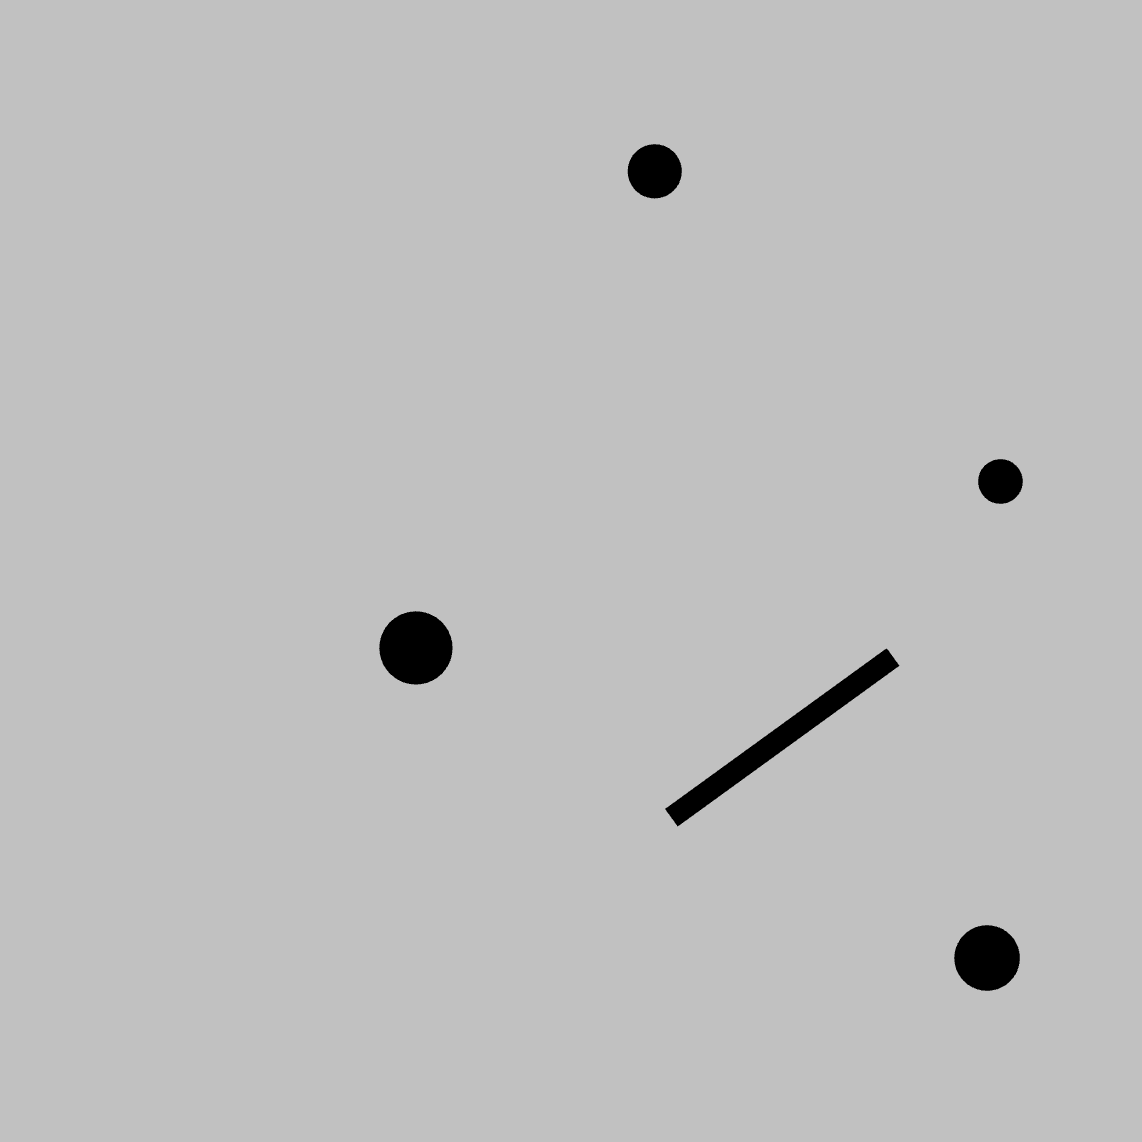
\includegraphics[width=0.15\linewidth]{graphics/test_model_05_1.png}
				\hfill
				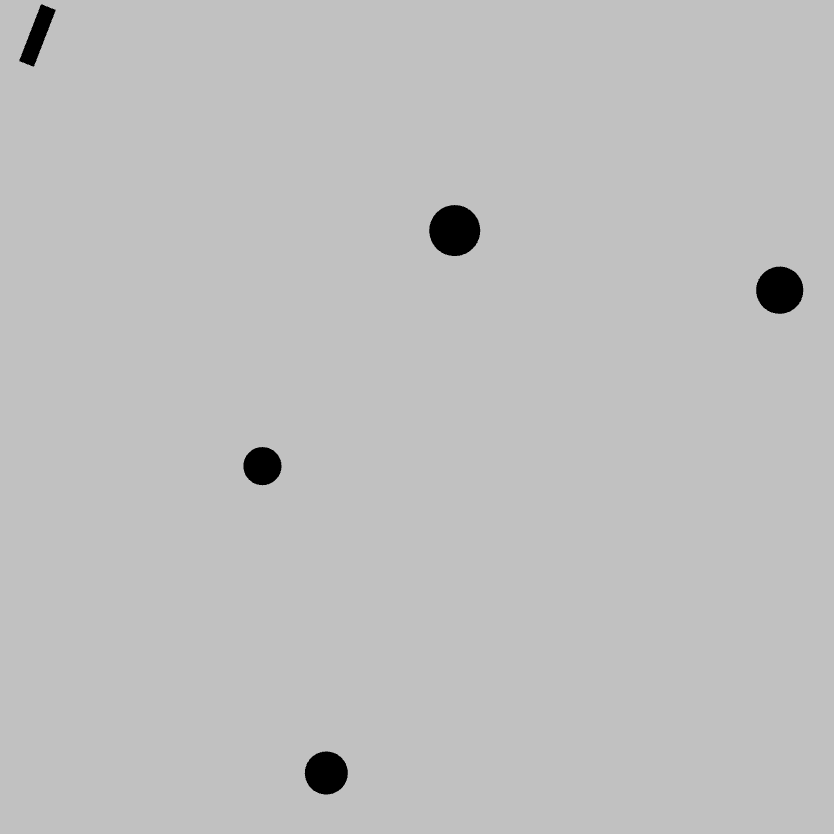
\includegraphics[width=0.15\linewidth]{graphics/test_model_05_2.png}
				\hfill
				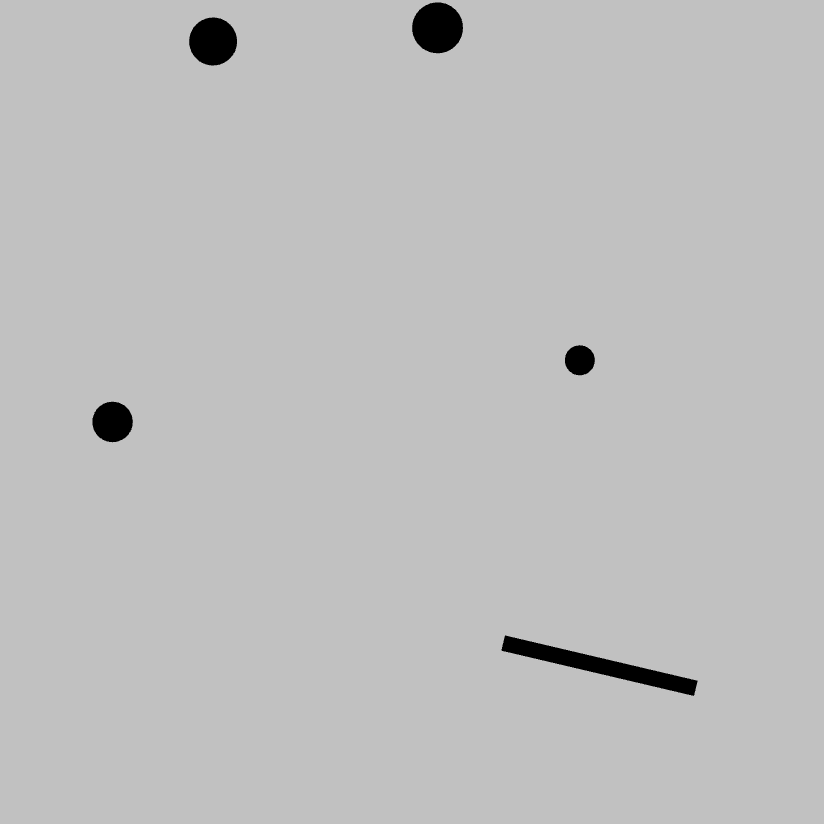
\includegraphics[width=0.15\linewidth]{graphics/test_model_05_3.png}
				\hfill
				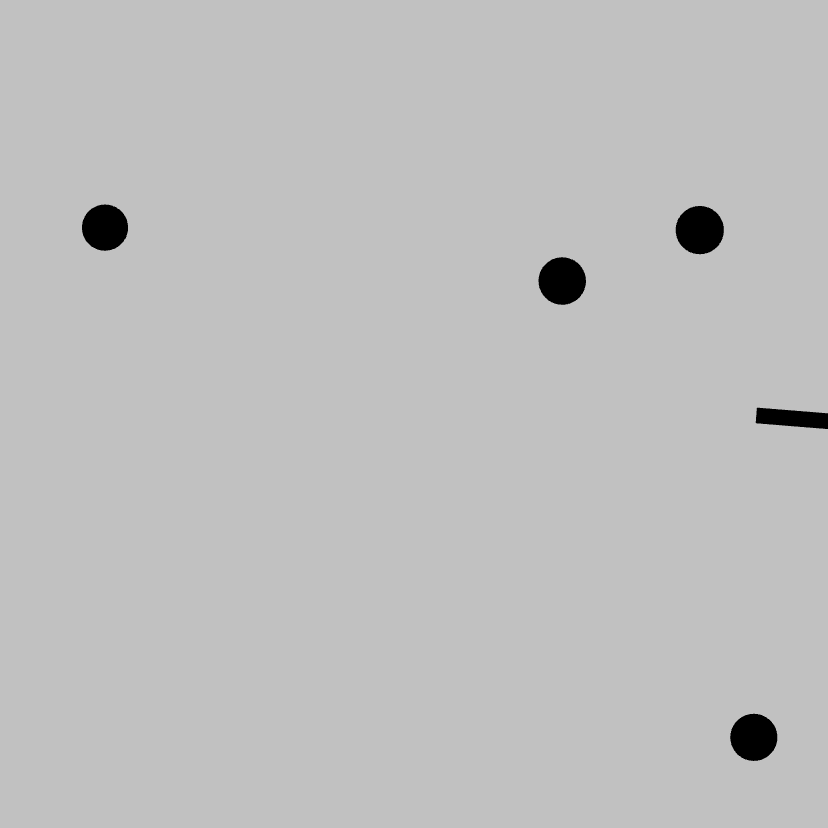
\includegraphics[width=0.15\linewidth]{graphics/test_model_05_4.png}
				\hfill
				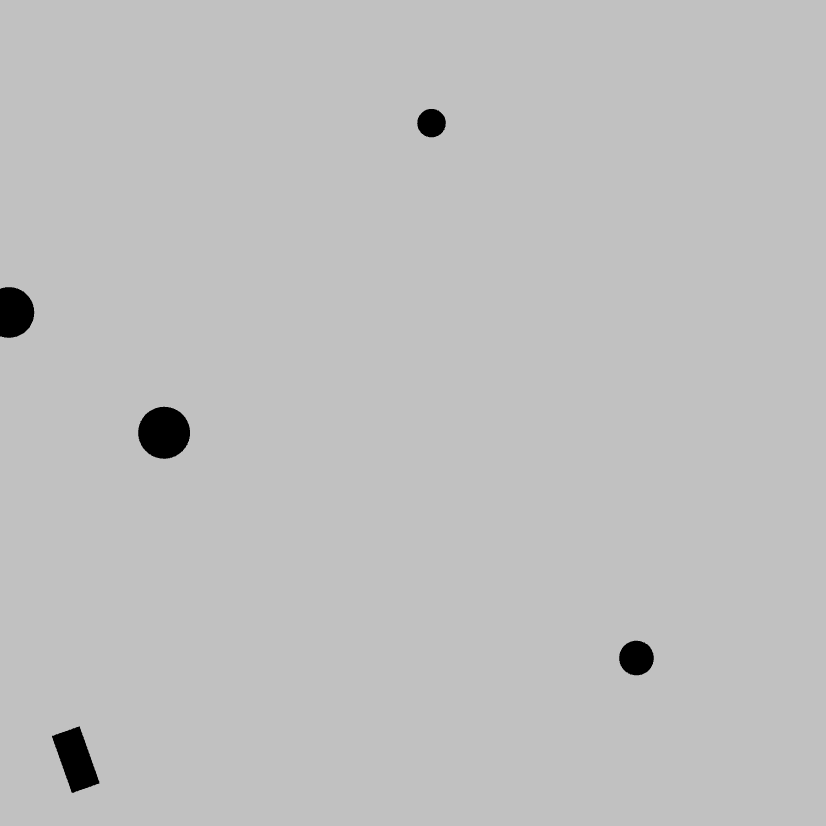
\includegraphics[width=0.15\linewidth]{graphics/test_model_05_5.png}
				\caption{Mondes de test avec 5 zones de corrosion.}
				\label{fig:test_model_05_5}
			\end{subfigure}
			\hfill
			\begin{subfigure}[t]{\linewidth}
				\centering
				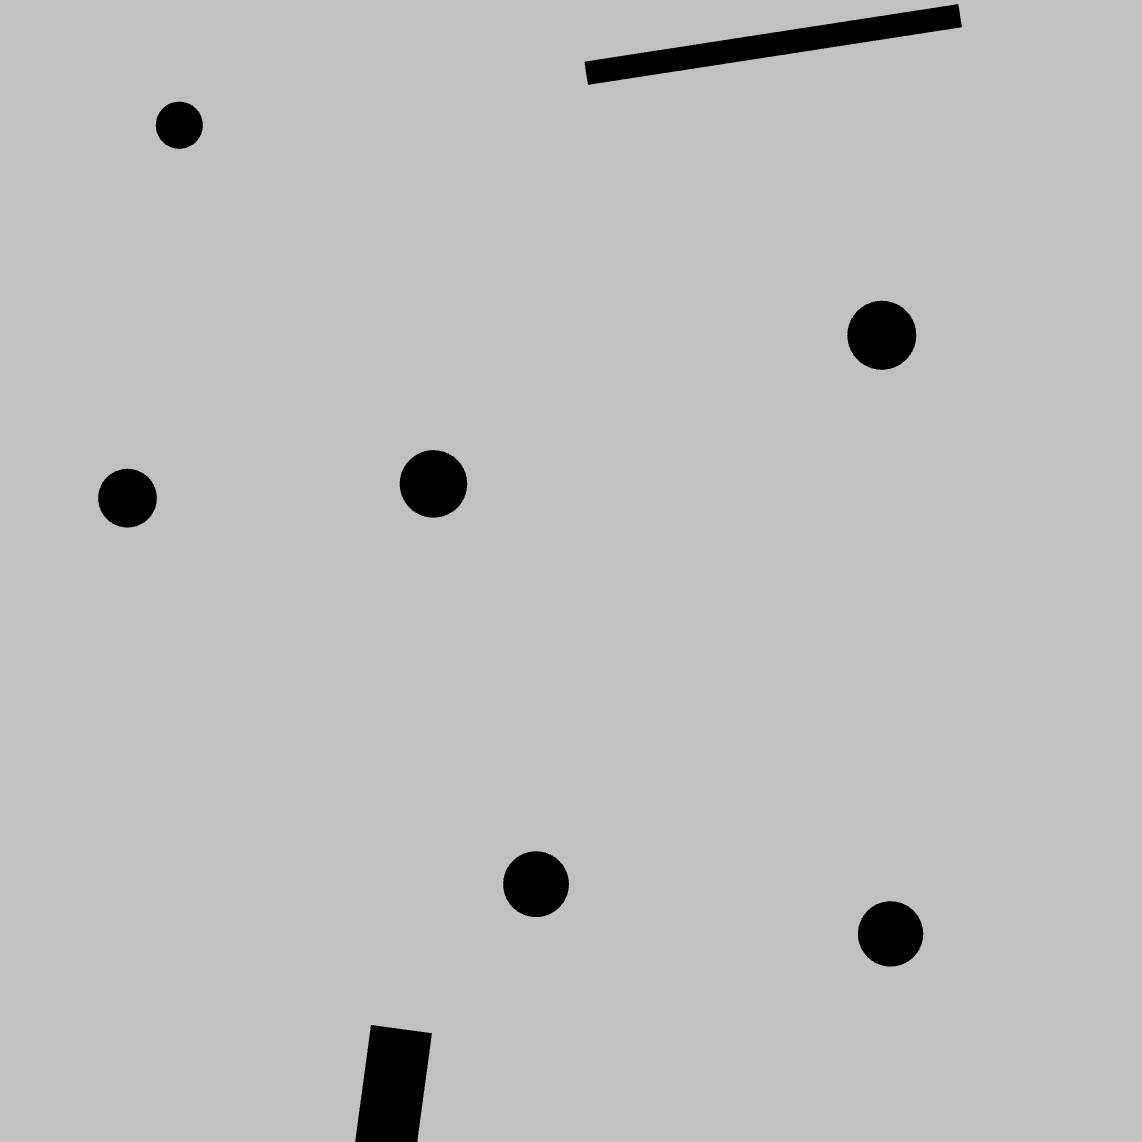
\includegraphics[width=0.15\linewidth]{graphics/test_model_08_1.png}
				\hfill
				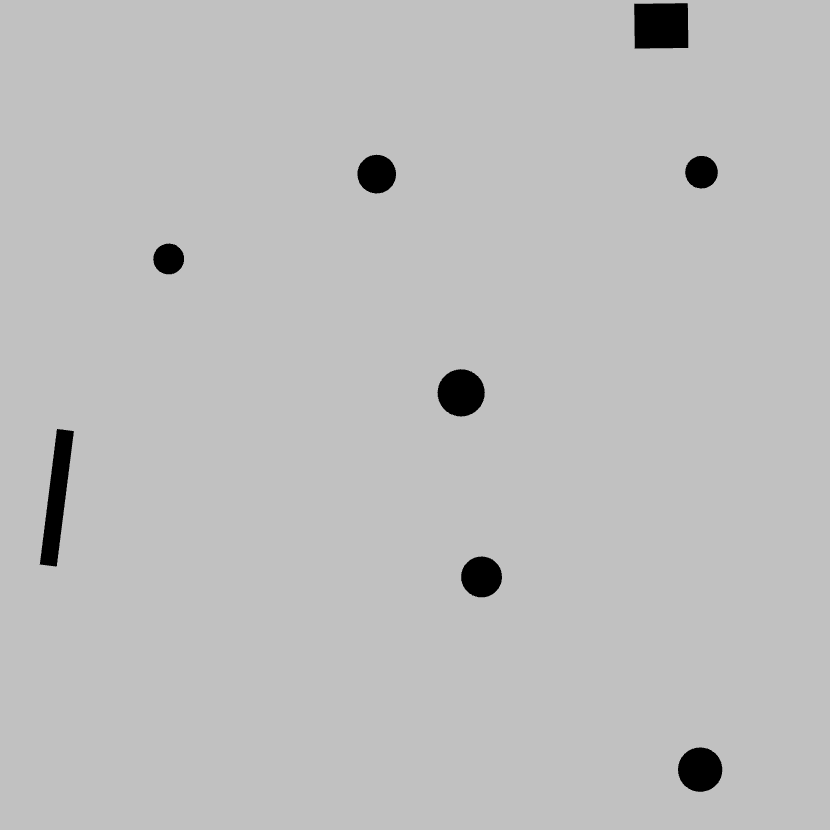
\includegraphics[width=0.15\linewidth]{graphics/test_model_08_2.png}
				\hfill
				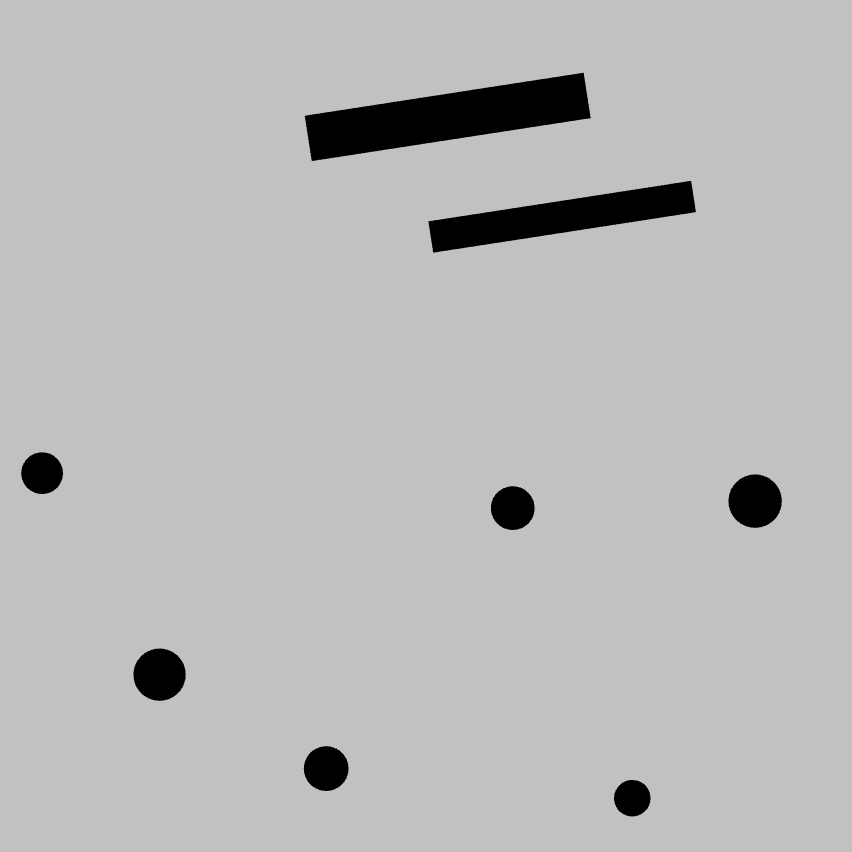
\includegraphics[width=0.15\linewidth]{graphics/test_model_08_3.png}
				\hfill
				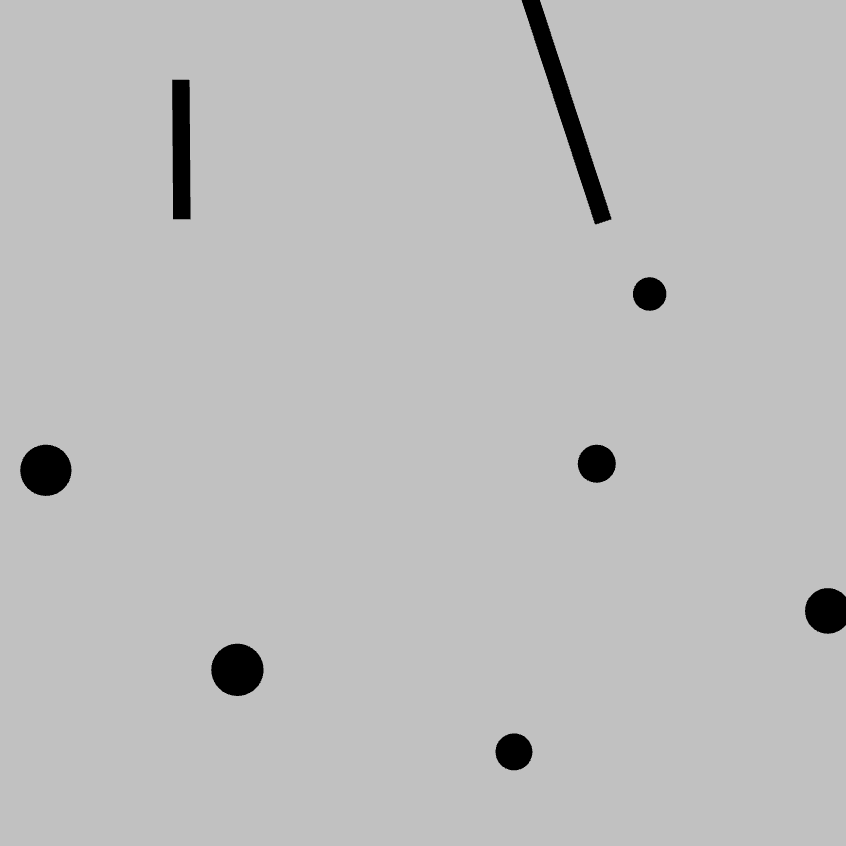
\includegraphics[width=0.15\linewidth]{graphics/test_model_08_4.png}
				\hfill
				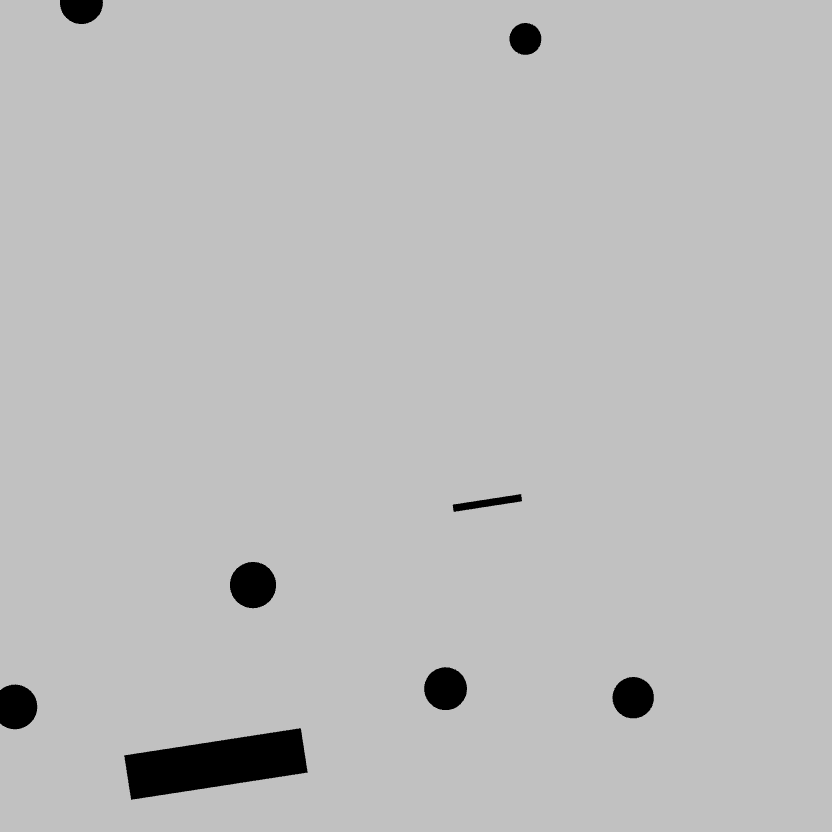
\includegraphics[width=0.15\linewidth]{graphics/test_model_08_5.png}
				\caption{Mondes de test avec 8 zones de corrosion.}
				\label{fig:test_model_08_5}
			\end{subfigure}
			\hfill
			\begin{subfigure}[t]{\linewidth}
				\centering
				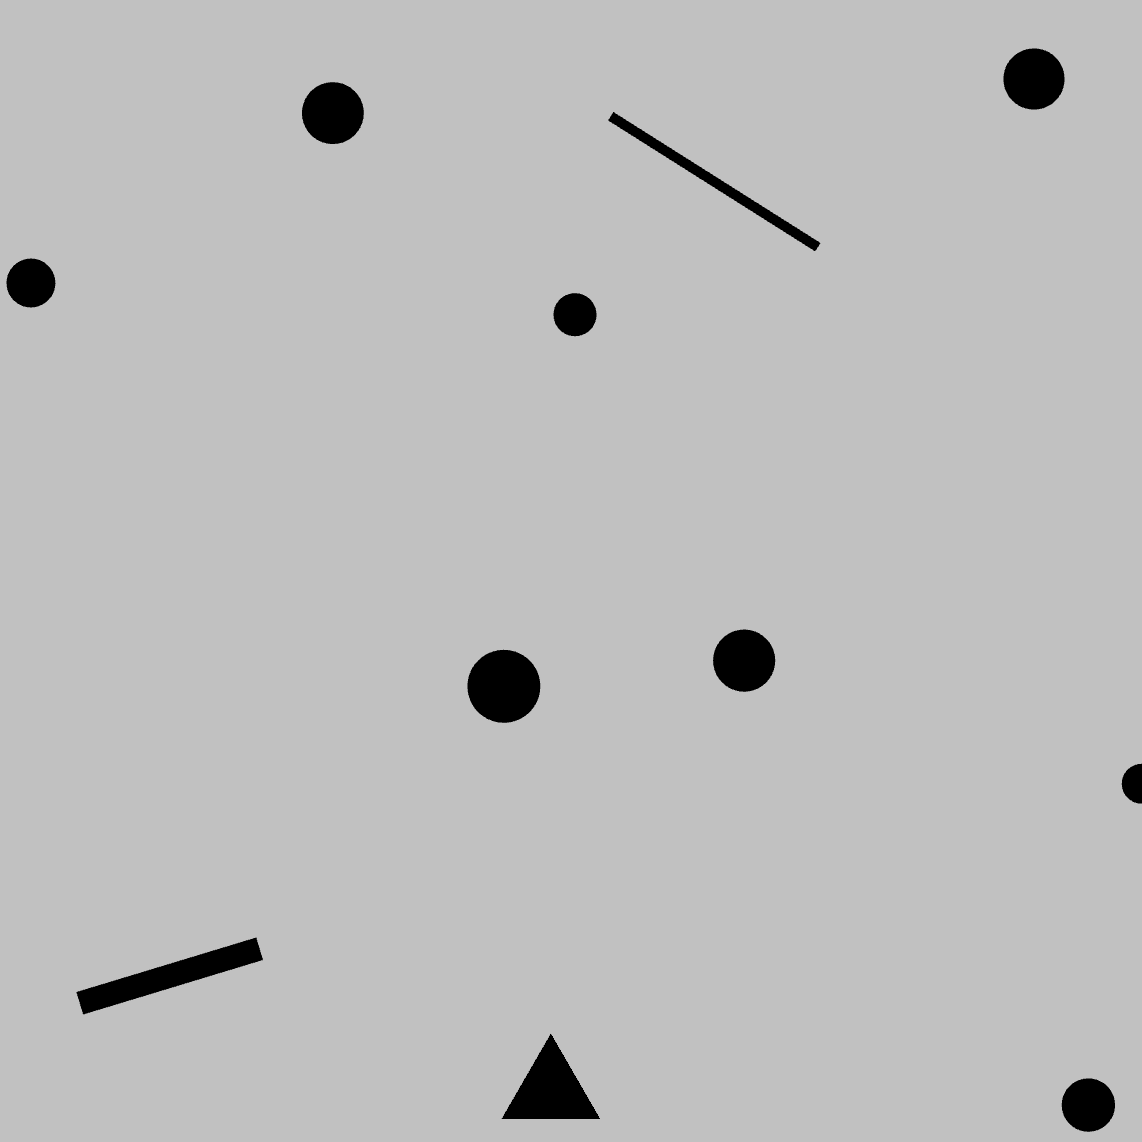
\includegraphics[width=0.15\linewidth]{graphics/test_model_11_1.png}
				\hfill
				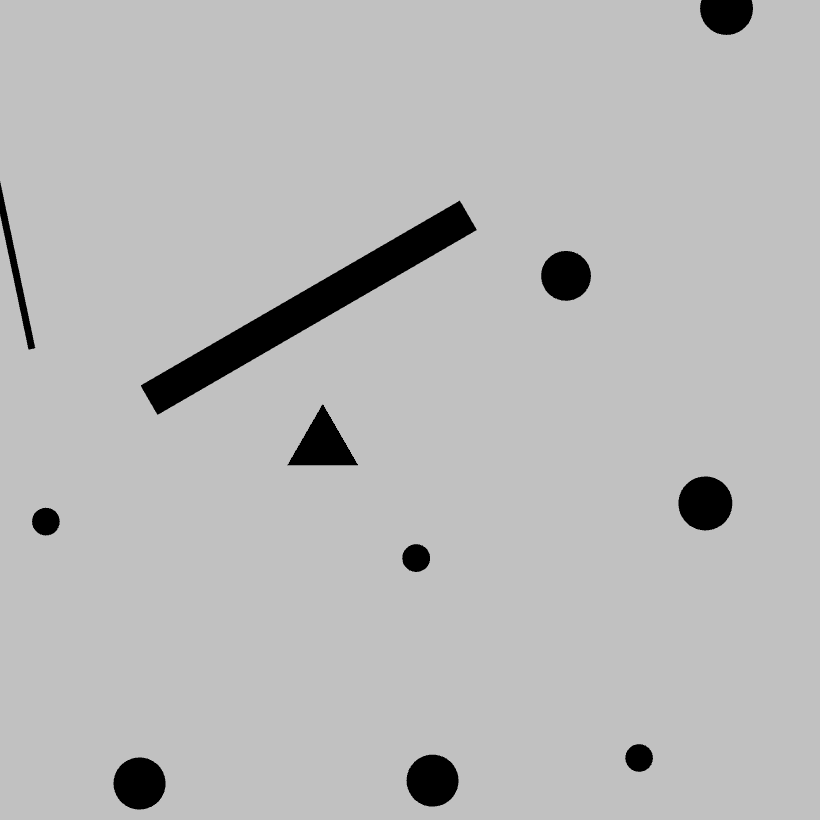
\includegraphics[width=0.15\linewidth]{graphics/test_model_11_2.png}
				\hfill
				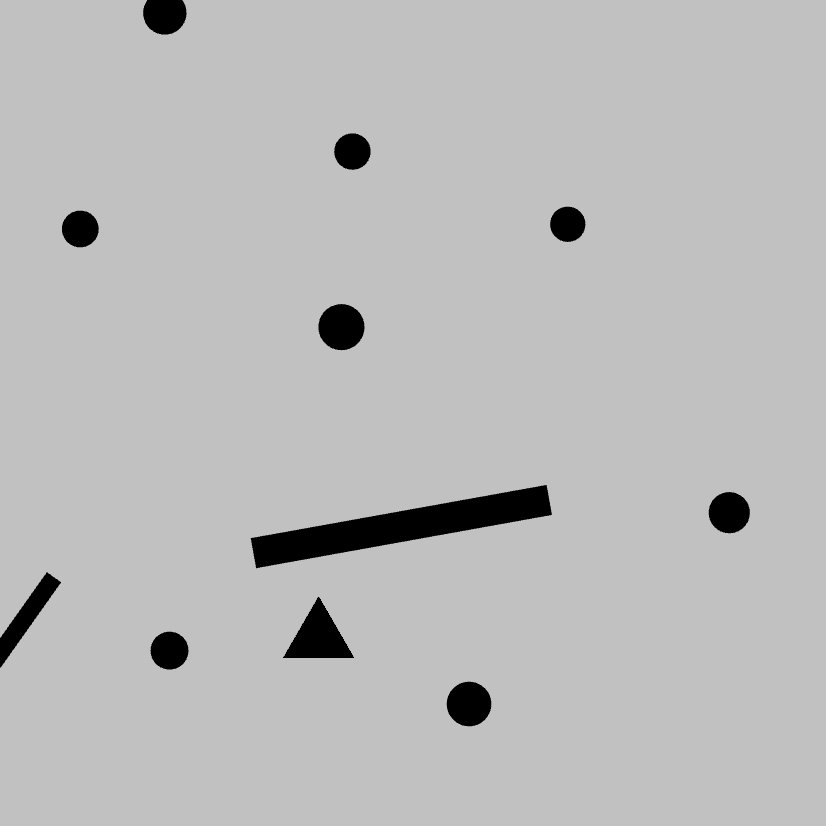
\includegraphics[width=0.15\linewidth]{graphics/test_model_11_3.png}
				\hfill
				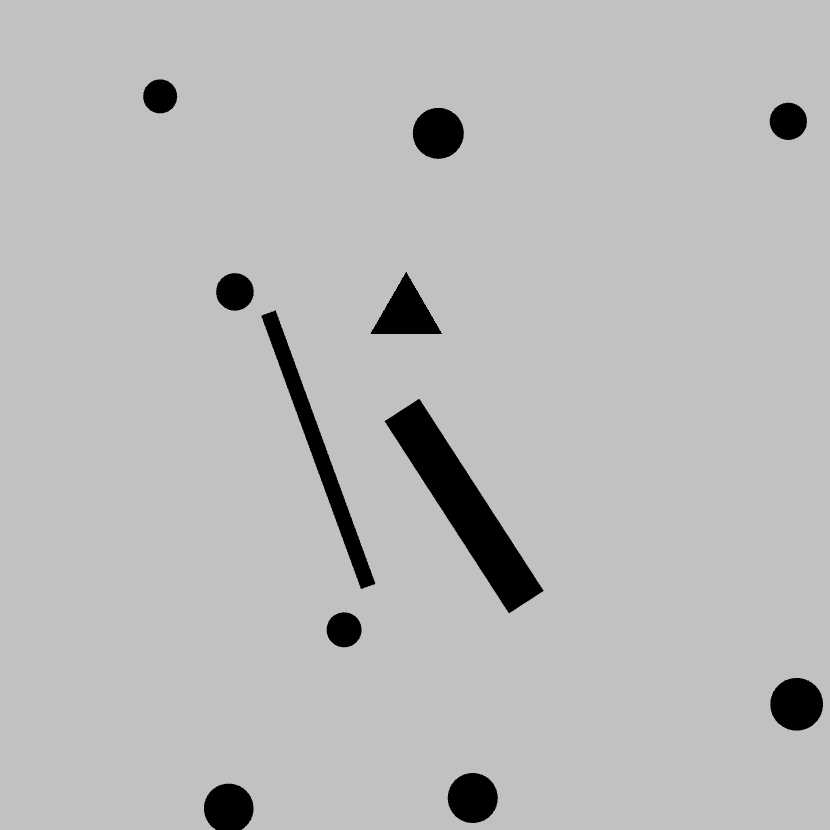
\includegraphics[width=0.15\linewidth]{graphics/test_model_11_4.png}
				\hfill
				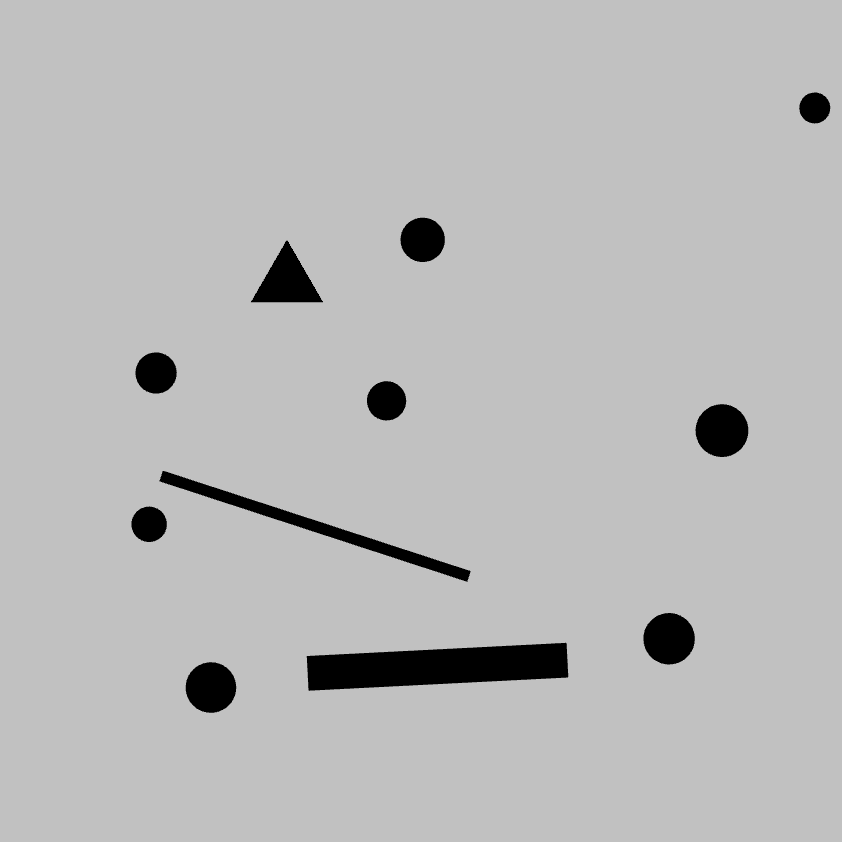
\includegraphics[width=0.15\linewidth]{graphics/test_model_11_5.png}
				\caption{Mondes de test avec 11 zones de corrosion.}
				\label{fig:test_model_11_5}
			\end{subfigure}
			\hfill
			\begin{subfigure}[t]{\linewidth}
				\centering
				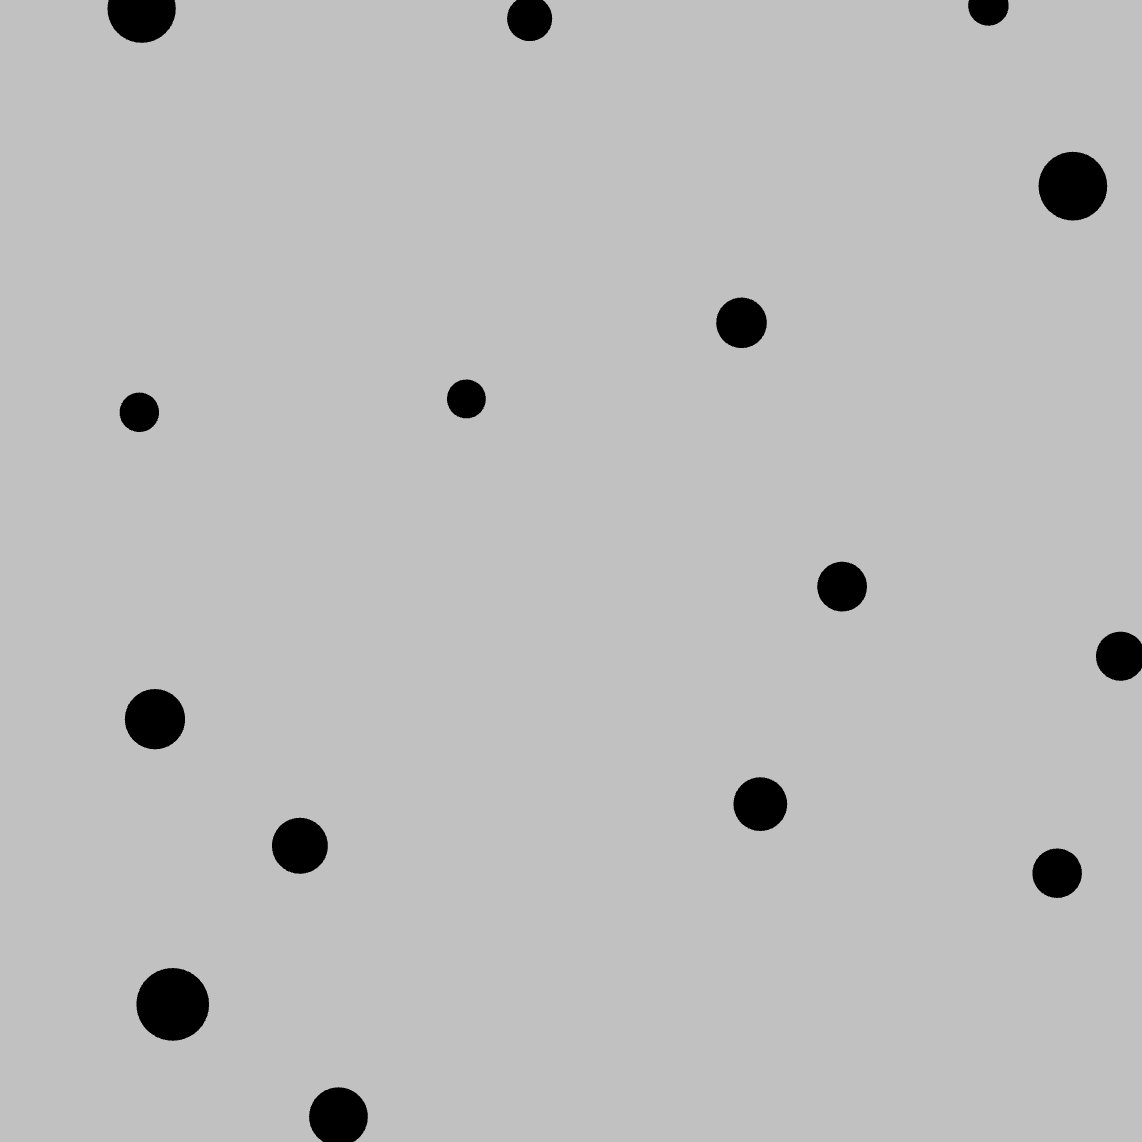
\includegraphics[width=0.15\linewidth]{graphics/test_model_15_1.png}
				\hfill
				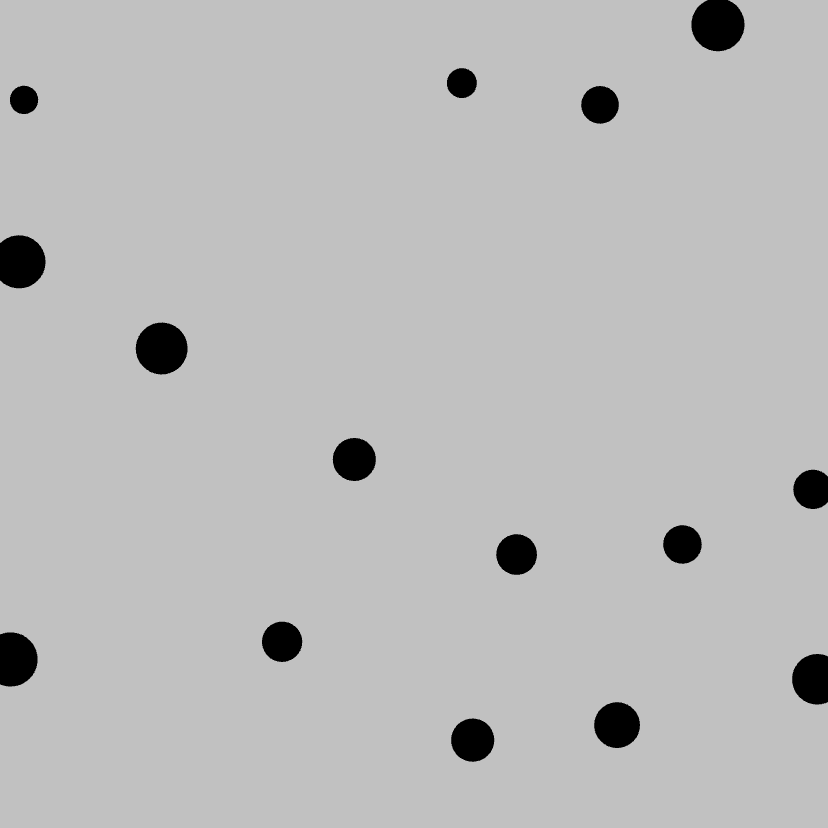
\includegraphics[width=0.15\linewidth]{graphics/test_model_15_2.png}
				\hfill
				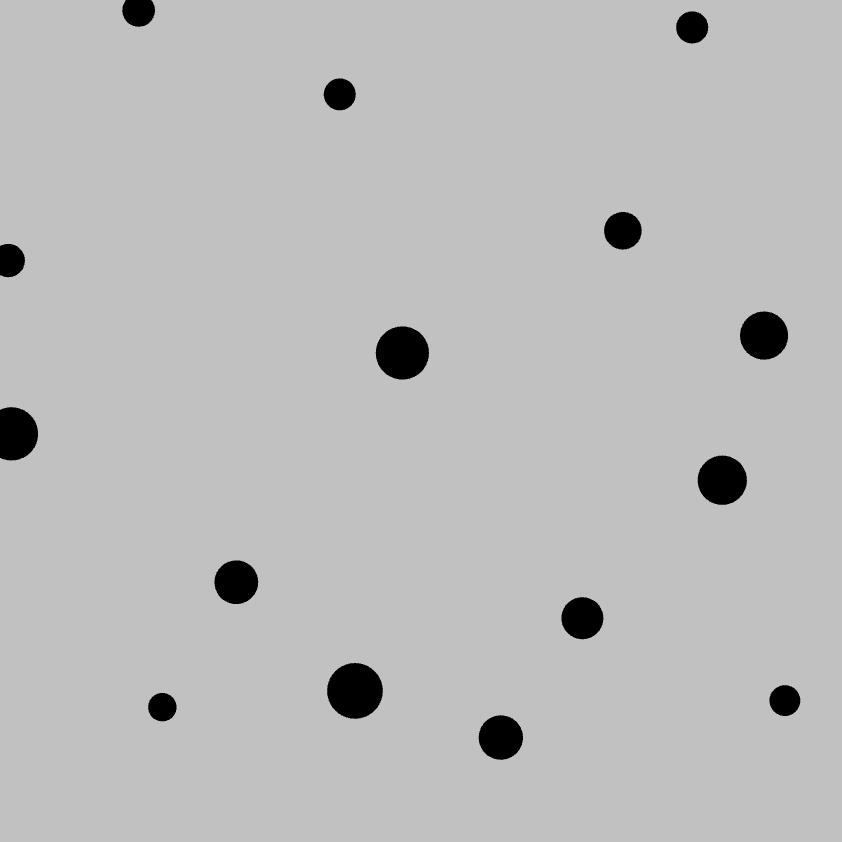
\includegraphics[width=0.15\linewidth]{graphics/test_model_15_3.png}
				\hfill
				\includegraphics[width=0.15\linewidth]{graphics/test_model_15_4.png}
				\hfill
				\includegraphics[width=0.15\linewidth]{graphics/test_model_15_5.png}
				\caption{Mondes de test avec 15 zones de corrosion.}
				\label{fig:test_model_15_5}
			\end{subfigure}
			\hfill
			\begin{subfigure}[t]{0.15\linewidth}
				\centering
				\includegraphics[width=\linewidth]{graphics/test_model_20_1.png}
				\caption{Mondes de test avec 20 zones de corrosion.}
				\label{fig:test_model_20_1}
			\end{subfigure}
			\hfill
			\begin{subfigure}[t]{0.15\linewidth}
				\centering
				\includegraphics[width=\linewidth]{graphics/test_model_30_1.png}
				\caption{Mondes de test avec 30 zones de corrosion.}
				\label{fig:test_model_30_1}
			\end{subfigure}
			\hfill
			\begin{subfigure}[t]{0.15\linewidth}
					\includegraphics[width=\linewidth]{graphics/test_model_11_complex_1.png}
					\caption{Mondes de test avec 11 zones de corrosion complexes.}
					\label{fig:test_model_11_complex_1}
			\end{subfigure}
			\hfill
			\begin{subfigure}[t]{0.15\linewidth}
				\centering
				\includegraphics[width=\linewidth]{graphics/test_model_15_complex_1.png}
				\caption{Mondes de test avec 15 zones de corrosion complexes.}
				\label{fig:test_model_15_complex_1}
			\end{subfigure}
			\caption{Différents environnements de test.}
			\label{fig:test_models}
		\end{figure}
	\section{Comparaison des différentes stratégies de navigation}
		\label{annexe:comparaison}
		\begin{figure}[H]
			\begin{subfigure}[t]{0.9\linewidth}
				\includegraphics[width=\linewidth]{graphics/investigation_polygonale-peinture_au_rouleau_ski_nordique-kappa_for_each_d_vs_investigation_polygonale-kappa_for_each_d.png}
				\caption{$\kappa$ en fonction de la densité du monde}
				\label{fig:investigation_polygonale-peinture_au_rouleau_ski_nordique-kappa_for_each_d_vs_investigation_polygonale-kappa_for_each_d}
			\end{subfigure}
			\hfill
			\begin{subfigure}[t]{0.9\linewidth}
					\includegraphics[width=\linewidth]{graphics/investigation_polygonale-peinture_au_rouleau_ski_nordique-time_for_each_d_vs_investigation_polygonale-time_for_each_d.png}
					\caption{Temps d'exécution en fonction de la densité du monde}
					\label{fig:investigation_polygonale-peinture_au_rouleau_ski_nordique-time_for_each_d_vs_investigation_polygonale-time_for_each_d}
			\end{subfigure}
			\caption{Évolution du $\kappa$ de Cohen et du temps d'exécution des différents algorithmes en fonction de la densité du monde pour différentes distances entre les crawlers.}
			\label{fig:investigation_polygonale-peinture_au_rouleau_ski_nordique_for_each_d}
		\end{figure}
	\section{Résultat d'investigation}
		\label{annexe:resultat}
		\begin{figure}[H]
			\centering
			\begin{subfigure}[t]{\linewidth}
				\centering
				\begin{subfigure}[t]{0.12\linewidth}
					\includegraphics[width=\linewidth]{../tests/peinture_au_rouleau-test_model_05_1-1.0/both.png}
				\end{subfigure}
				\hfill
				\begin{subfigure}[t]{0.11\linewidth}
					\includegraphics[width=\linewidth]{../tests/peinture_au_rouleau-test_model_08_1-1.0/both.png}
				\end{subfigure}
				\hfill
				\begin{subfigure}[t]{0.11\linewidth}
					\includegraphics[width=\linewidth]{../tests/peinture_au_rouleau-test_model_11_1-1.0/both.png}
				\end{subfigure}
				\hfill
				\begin{subfigure}[t]{0.11\linewidth}
					\includegraphics[width=\linewidth]{../tests/peinture_au_rouleau-test_model_15_1-1.0/both.png}
				\end{subfigure}
				\hfill
				\begin{subfigure}[t]{0.11\linewidth}
					\includegraphics[width=\linewidth]{../tests/peinture_au_rouleau-test_model_20_1-1.0/both.png}
				\end{subfigure}
				\hfill
				\begin{subfigure}[t]{0.11\linewidth}
					\includegraphics[width=\linewidth]{../tests/peinture_au_rouleau-test_model_30_1-1.0/both.png}
				\end{subfigure}
				\hfill
				\begin{subfigure}[t]{0.11\linewidth}
					\includegraphics[width=\linewidth]{../tests/peinture_au_rouleau-test_model_11_complex_1-1.0/both.png}
				\end{subfigure}
				\hfill
				\begin{subfigure}[t]{0.11\linewidth}
					\includegraphics[width=\linewidth]{../tests/peinture_au_rouleau-test_model_15_complex_1-1.0/both.png}
				\end{subfigure}
				\caption{$d = 1$ m}
			\end{subfigure}
			\hfill
			\begin{subfigure}[t]{\linewidth}
				\centering
				\begin{subfigure}[t]{0.11\linewidth}
					\includegraphics[width=\linewidth]{../tests/peinture_au_rouleau-test_model_05_1-2.0/both.png}
				\end{subfigure}
				\hfill
				\begin{subfigure}[t]{0.11\linewidth}
					\includegraphics[width=\linewidth]{../tests/peinture_au_rouleau-test_model_08_1-2.0/both.png}
				\end{subfigure}
				\hfill
				\begin{subfigure}[t]{0.11\linewidth}
					\includegraphics[width=\linewidth]{../tests/peinture_au_rouleau-test_model_11_1-2.0/both.png}
				\end{subfigure}
				\hfill
				\begin{subfigure}[t]{0.11\linewidth}
					\includegraphics[width=\linewidth]{../tests/peinture_au_rouleau-test_model_15_1-2.0/both.png}
				\end{subfigure}
				\hfill
				\begin{subfigure}[t]{0.1\linewidth}
					\includegraphics[width=\linewidth]{../tests/peinture_au_rouleau-test_model_20_1-2.0/both.png}
				\end{subfigure}
				\hfill
				\begin{subfigure}[t]{0.11\linewidth}
					\includegraphics[width=\linewidth]{../tests/peinture_au_rouleau-test_model_30_1-2.0/both.png}
				\end{subfigure}
				\hfill
				\begin{subfigure}[t]{0.11\linewidth}
					\includegraphics[width=\linewidth]{../tests/peinture_au_rouleau-test_model_11_complex_1-2.0/both.png}
				\end{subfigure}
				\hfill
				\begin{subfigure}[t]{0.11\linewidth}
					\includegraphics[width=\linewidth]{../tests/peinture_au_rouleau-test_model_15_complex_1-2.0/both.png}
				\end{subfigure}
				\caption{$d = 2$ m}
			\end{subfigure}
			\hfill
			\begin{subfigure}[t]{\linewidth}
				\centering
				\begin{subfigure}[t]{0.11\linewidth}
					\includegraphics[width=\linewidth]{../tests/peinture_au_rouleau-test_model_05_1-3.0/both.png}
				\end{subfigure}
				\hfill
				\begin{subfigure}[t]{0.11\linewidth}
					\includegraphics[width=\linewidth]{../tests/peinture_au_rouleau-test_model_08_1-3.0/both.png}
				\end{subfigure}
				\hfill
				\begin{subfigure}[t]{0.11\linewidth}
					\includegraphics[width=\linewidth]{../tests/peinture_au_rouleau-test_model_11_1-3.0/both.png}
				\end{subfigure}
				\hfill
				\begin{subfigure}[t]{0.11\linewidth}
					\includegraphics[width=\linewidth]{../tests/peinture_au_rouleau-test_model_15_1-3.0/both.png}
				\end{subfigure}
				\hfill
				\begin{subfigure}[t]{0.11\linewidth}
					\includegraphics[width=\linewidth]{../tests/peinture_au_rouleau-test_model_20_1-3.0/both.png}
				\end{subfigure}
				\hfill
				\begin{subfigure}[t]{0.11\linewidth}
					\includegraphics[width=\linewidth]{../tests/peinture_au_rouleau-test_model_30_1-3.0/both.png}
				\end{subfigure}
				\hfill
				\begin{subfigure}[t]{0.11\linewidth}
					\includegraphics[width=\linewidth]{../tests/peinture_au_rouleau-test_model_11_complex_1-3.0/both.png}
				\end{subfigure}
				\hfill
				\begin{subfigure}[t]{0.11\linewidth}
					\includegraphics[width=\linewidth]{../tests/peinture_au_rouleau-test_model_15_complex_1-3.0/both.png}
				\end{subfigure}
				\caption{$d = 3$ m}
			\end{subfigure}
			\hfill
			\begin{subfigure}[t]{\linewidth}
				\centering
				\begin{subfigure}[t]{0.11\linewidth}
					\includegraphics[width=\linewidth]{../tests/peinture_au_rouleau-test_model_05_1-6.0/both.png}
				\end{subfigure}
				\hfill
				\begin{subfigure}[t]{0.11\linewidth}
					\includegraphics[width=\linewidth]{../tests/peinture_au_rouleau-test_model_08_1-6.0/both.png}
				\end{subfigure}
				\hfill
				\begin{subfigure}[t]{0.11\linewidth}
					\includegraphics[width=\linewidth]{../tests/peinture_au_rouleau-test_model_11_1-6.0/both.png}
				\end{subfigure}
				\hfill
				\begin{subfigure}[t]{0.11\linewidth}
					\includegraphics[width=\linewidth]{../tests/peinture_au_rouleau-test_model_15_1-6.0/both.png}
				\end{subfigure}
				\hfill
				\begin{subfigure}[t]{0.11\linewidth}
					\includegraphics[width=\linewidth]{../tests/peinture_au_rouleau-test_model_20_1-6.0/both.png}
				\end{subfigure}
				\hfill
				\begin{subfigure}[t]{0.11\linewidth}
					\includegraphics[width=\linewidth]{../tests/peinture_au_rouleau-test_model_30_1-6.0/both.png}
				\end{subfigure}
				\hfill
				\begin{subfigure}[t]{0.11\linewidth}
					\includegraphics[width=\linewidth]{../tests/peinture_au_rouleau-test_model_11_complex_1-6.0/both.png}
				\end{subfigure}
				\hfill
				\begin{subfigure}[t]{0.11\linewidth}
					\includegraphics[width=\linewidth]{../tests/peinture_au_rouleau-test_model_15_complex_1-6.0/both.png}
				\end{subfigure}
				\caption{$d = 6$ m}
			\end{subfigure}
			\caption{Superposition des cartes d'investigation avec la cartographie des zones de corrosion obtenue pour les différents mondes de test, pour la méthode \textit{peinture au rouleau}.}
			\label{fig:peinture_au_rouleau_resultats}
		\end{figure}

		\begin{figure}[H]
			\centering
			\begin{subfigure}[t]{\linewidth}
				\centering
				\begin{subfigure}[t]{0.11\linewidth}
					\includegraphics[width=\linewidth]{../tests/ski_nordique-test_model_05_1-1.0-3.0/both.png}
				\end{subfigure}
				\hfill
				\begin{subfigure}[t]{0.11\linewidth}
					\includegraphics[width=\linewidth]{../tests/ski_nordique-test_model_08_1-1.0-3.0/both.png}
				\end{subfigure}
				\hfill
				\begin{subfigure}[t]{0.11\linewidth}
					\includegraphics[width=\linewidth]{../tests/ski_nordique-test_model_11_1-1.0-3.0/both.png}
				\end{subfigure}
				\hfill
				\begin{subfigure}[t]{0.11\linewidth}
					\includegraphics[width=\linewidth]{../tests/ski_nordique-test_model_15_1-1.0-3.0/both.png}
				\end{subfigure}
				\hfill
				\begin{subfigure}[t]{0.11\linewidth}
					\includegraphics[width=\linewidth]{../tests/ski_nordique-test_model_20_1-1.0-3.0/both.png}
				\end{subfigure}
				\hfill
				\begin{subfigure}[t]{0.11\linewidth}
					\includegraphics[width=\linewidth]{../tests/ski_nordique-test_model_30_1-1.0-3.0/both.png}
				\end{subfigure}
				\hfill
				\begin{subfigure}[t]{0.11\linewidth}
					\includegraphics[width=\linewidth]{../tests/ski_nordique-test_model_11_complex_1-1.0-3.0/both.png}
				\end{subfigure}
				\hfill
				\begin{subfigure}[t]{0.11\linewidth}
					\includegraphics[width=\linewidth]{../tests/ski_nordique-test_model_15_complex_1-1.0-3.0/both.png}
				\end{subfigure}
				\caption{$d = 1$ m, $s = 3$ m}
			\end{subfigure}
			\hfill
			\begin{subfigure}[t]{\linewidth}
				\centering
				\begin{subfigure}[t]{0.11\linewidth}
					\includegraphics[width=\linewidth]{../tests/ski_nordique-test_model_05_1-2.0-3.0/both.png}
				\end{subfigure}
				\hfill
				\begin{subfigure}[t]{0.11\linewidth}
					\includegraphics[width=\linewidth]{../tests/ski_nordique-test_model_08_1-2.0-3.0/both.png}
				\end{subfigure}
				\hfill
				\begin{subfigure}[t]{0.11\linewidth}
					\includegraphics[width=\linewidth]{../tests/ski_nordique-test_model_11_1-2.0-3.0/both.png}
				\end{subfigure}
				\hfill
				\begin{subfigure}[t]{0.11\linewidth}
					\includegraphics[width=\linewidth]{../tests/ski_nordique-test_model_15_1-2.0-3.0/both.png}
				\end{subfigure}
				\hfill
				\begin{subfigure}[t]{0.11\linewidth}
					\includegraphics[width=\linewidth]{../tests/ski_nordique-test_model_20_1-2.0-3.0/both.png}
				\end{subfigure}
				\hfill
				\begin{subfigure}[t]{0.11\linewidth}
					\includegraphics[width=\linewidth]{../tests/ski_nordique-test_model_30_1-2.0-3.0/both.png}
				\end{subfigure}
				\hfill
				\begin{subfigure}[t]{0.11\linewidth}
					\includegraphics[width=\linewidth]{../tests/ski_nordique-test_model_11_complex_1-2.0-3.0/both.png}
				\end{subfigure}
				\hfill
				\begin{subfigure}[t]{0.11\linewidth}
					\includegraphics[width=\linewidth]{../tests/ski_nordique-test_model_15_complex_1-2.0-3.0/both.png}
				\end{subfigure}
				\caption{$d = 2$ m, $s = 3$ m}
			\end{subfigure}
			\hfill
			\begin{subfigure}[t]{\linewidth}
				\centering
				\begin{subfigure}[t]{0.11\linewidth}
					\includegraphics[width=\linewidth]{../tests/ski_nordique-test_model_05_1-3.0-3.0/both.png}
				\end{subfigure}
				\hfill
				\begin{subfigure}[t]{0.11\linewidth}
					\includegraphics[width=\linewidth]{../tests/ski_nordique-test_model_08_1-3.0-3.0/both.png}
				\end{subfigure}
				\hfill
				\begin{subfigure}[t]{0.11\linewidth}
					\includegraphics[width=\linewidth]{../tests/ski_nordique-test_model_11_1-3.0-3.0/both.png}
				\end{subfigure}
				\hfill
				\begin{subfigure}[t]{0.11\linewidth}
					\includegraphics[width=\linewidth]{../tests/ski_nordique-test_model_15_1-3.0-3.0/both.png}
				\end{subfigure}
				\hfill
				\begin{subfigure}[t]{0.11\linewidth}
					\includegraphics[width=\linewidth]{../tests/ski_nordique-test_model_20_1-3.0-3.0/both.png}
				\end{subfigure}
				\hfill
				\begin{subfigure}[t]{0.11\linewidth}
					\includegraphics[width=\linewidth]{../tests/ski_nordique-test_model_30_1-3.0-3.0/both.png}
				\end{subfigure}
				\hfill
				\begin{subfigure}[t]{0.11\linewidth}
					\includegraphics[width=\linewidth]{../tests/ski_nordique-test_model_11_complex_1-3.0-3.0/both.png}
				\end{subfigure}
				\hfill
				\begin{subfigure}[t]{0.11\linewidth}
					\includegraphics[width=\linewidth]{../tests/ski_nordique-test_model_15_complex_1-3.0-3.0/both.png}
				\end{subfigure}
				\caption{$d = 3$ m, $s = 3$ m}
			\end{subfigure}
			\hfill
			\begin{subfigure}[t]{\linewidth}
				\centering
				\begin{subfigure}[t]{0.11\linewidth}
					\includegraphics[width=\linewidth]{../tests/ski_nordique-test_model_05_1-6.0-3.0/both.png}
				\end{subfigure}
				\hfill
				\begin{subfigure}[t]{0.11\linewidth}
					\includegraphics[width=\linewidth]{../tests/ski_nordique-test_model_08_1-6.0-3.0/both.png}
				\end{subfigure}
				\hfill
				\begin{subfigure}[t]{0.11\linewidth}
					\includegraphics[width=\linewidth]{../tests/ski_nordique-test_model_11_1-6.0-3.0/both.png}
				\end{subfigure}
				\hfill
				\begin{subfigure}[t]{0.11\linewidth}
					\includegraphics[width=\linewidth]{../tests/ski_nordique-test_model_15_1-6.0-3.0/both.png}
				\end{subfigure}
				\hfill
				\begin{subfigure}[t]{0.11\linewidth}
					\includegraphics[width=\linewidth]{../tests/ski_nordique-test_model_20_1-6.0-3.0/both.png}
				\end{subfigure}
				\hfill
				\begin{subfigure}[t]{0.11\linewidth}
					\includegraphics[width=\linewidth]{../tests/ski_nordique-test_model_30_1-6.0-3.0/both.png}
				\end{subfigure}
				\hfill
				\begin{subfigure}[t]{0.11\linewidth}
					\includegraphics[width=\linewidth]{../tests/ski_nordique-test_model_11_complex_1-6.0-3.0/both.png}
				\end{subfigure}
				\hfill
				\begin{subfigure}[t]{0.11\linewidth}
					\includegraphics[width=\linewidth]{../tests/ski_nordique-test_model_15_complex_1-6.0-3.0/both.png}
				\end{subfigure}
				\caption{$d = 6$ m, $s = 3$ m}
			\end{subfigure}
			\caption{Superposition des cartes d'investigation avec la cartographie des zones de corrosion obtenue pour les différents mondes de test, pour la méthode \textit{ski nordique} - 1.}
			\label{fig:ski_nordique_resultats}
		\end{figure}

		\begin{figure}[H]
			\centering
			\begin{subfigure}[t]{\linewidth}
				\centering
				\begin{subfigure}[t]{0.11\linewidth}
					\includegraphics[width=\linewidth]{../tests/ski_nordique-test_model_05_1-3.0-1.0/both.png}
				\end{subfigure}
				\hfill
				\begin{subfigure}[t]{0.11\linewidth}
					\includegraphics[width=\linewidth]{../tests/ski_nordique-test_model_08_1-3.0-1.0/both.png}
				\end{subfigure}
				\hfill
				\begin{subfigure}[t]{0.11\linewidth}
					\includegraphics[width=\linewidth]{../tests/ski_nordique-test_model_11_1-3.0-1.0/both.png}
				\end{subfigure}
				\hfill
				\begin{subfigure}[t]{0.11\linewidth}
					\includegraphics[width=\linewidth]{../tests/ski_nordique-test_model_15_1-3.0-1.0/both.png}
				\end{subfigure}
				\hfill
				\begin{subfigure}[t]{0.11\linewidth}
					\includegraphics[width=\linewidth]{../tests/ski_nordique-test_model_20_1-3.0-1.0/both.png}
				\end{subfigure}
				\hfill
				\begin{subfigure}[t]{0.11\linewidth}
					\includegraphics[width=\linewidth]{../tests/ski_nordique-test_model_30_1-3.0-1.0/both.png}
				\end{subfigure}
				\hfill
				\begin{subfigure}[t]{0.11\linewidth}
					\includegraphics[width=\linewidth]{../tests/ski_nordique-test_model_11_complex_1-3.0-1.0/both.png}
				\end{subfigure}
				\hfill
				\begin{subfigure}[t]{0.11\linewidth}
					\includegraphics[width=\linewidth]{../tests/ski_nordique-test_model_15_complex_1-3.0-1.0/both.png}
				\end{subfigure}
				\caption{$d = 3$ m, $s = 1$ m}
			\end{subfigure}
			\hfill
			\begin{subfigure}[t]{\linewidth}
				\centering
				\begin{subfigure}[t]{0.11\linewidth}
					\includegraphics[width=\linewidth]{../tests/ski_nordique-test_model_05_1-3.0-2.0/both.png}
				\end{subfigure}
				\hfill
				\begin{subfigure}[t]{0.11\linewidth}
					\includegraphics[width=\linewidth]{../tests/ski_nordique-test_model_08_1-3.0-2.0/both.png}
				\end{subfigure}
				\hfill
				\begin{subfigure}[t]{0.11\linewidth}
					\includegraphics[width=\linewidth]{../tests/ski_nordique-test_model_11_1-3.0-2.0/both.png}
				\end{subfigure}
				\hfill
				\begin{subfigure}[t]{0.11\linewidth}
					\includegraphics[width=\linewidth]{../tests/ski_nordique-test_model_15_1-3.0-2.0/both.png}
				\end{subfigure}
				\hfill
				\begin{subfigure}[t]{0.11\linewidth}
					\includegraphics[width=\linewidth]{../tests/ski_nordique-test_model_20_1-3.0-2.0/both.png}
				\end{subfigure}
				\hfill
				\begin{subfigure}[t]{0.11\linewidth}
					\includegraphics[width=\linewidth]{../tests/ski_nordique-test_model_30_1-3.0-2.0/both.png}
				\end{subfigure}
				\hfill
				\begin{subfigure}[t]{0.11\linewidth}
					\includegraphics[width=\linewidth]{../tests/ski_nordique-test_model_11_complex_1-3.0-2.0/both.png}
				\end{subfigure}
				\hfill
				\begin{subfigure}[t]{0.11\linewidth}
					\includegraphics[width=\linewidth]{../tests/ski_nordique-test_model_15_complex_1-3.0-2.0/both.png}
				\end{subfigure}
				\caption{$d = 3$ m, $s = 2$ m}
			\end{subfigure}
			\hfill
			\begin{subfigure}[t]{\linewidth}
				\centering
				\begin{subfigure}[t]{0.11\linewidth}
					\includegraphics[width=\linewidth]{../tests/ski_nordique-test_model_05_1-3.0-3.0/both.png}
				\end{subfigure}
				\hfill
				\begin{subfigure}[t]{0.11\linewidth}
					\includegraphics[width=\linewidth]{../tests/ski_nordique-test_model_08_1-3.0-3.0/both.png}
				\end{subfigure}
				\hfill
				\begin{subfigure}[t]{0.11\linewidth}
					\includegraphics[width=\linewidth]{../tests/ski_nordique-test_model_11_1-3.0-3.0/both.png}
				\end{subfigure}
				\hfill
				\begin{subfigure}[t]{0.11\linewidth}
					\includegraphics[width=\linewidth]{../tests/ski_nordique-test_model_15_1-3.0-3.0/both.png}
				\end{subfigure}
				\hfill
				\begin{subfigure}[t]{0.11\linewidth}
					\includegraphics[width=\linewidth]{../tests/ski_nordique-test_model_20_1-3.0-3.0/both.png}
				\end{subfigure}
				\hfill
				\begin{subfigure}[t]{0.11\linewidth}
					\includegraphics[width=\linewidth]{../tests/ski_nordique-test_model_30_1-3.0-3.0/both.png}
				\end{subfigure}
				\hfill
				\begin{subfigure}[t]{0.11\linewidth}
					\includegraphics[width=\linewidth]{../tests/ski_nordique-test_model_11_complex_1-3.0-3.0/both.png}
				\end{subfigure}
				\hfill
				\begin{subfigure}[t]{0.11\linewidth}
					\includegraphics[width=\linewidth]{../tests/ski_nordique-test_model_15_complex_1-3.0-3.0/both.png}
				\end{subfigure}
				\caption{$d = 3$ m, $s = 3$ m}
			\end{subfigure}
			\hfill
			\begin{subfigure}[t]{\linewidth}
				\centering
				\begin{subfigure}[t]{0.11\linewidth}
					\includegraphics[width=\linewidth]{../tests/ski_nordique-test_model_05_1-3.0-6.0/both.png}
				\end{subfigure}
				\hfill
				\begin{subfigure}[t]{0.11\linewidth}
					\includegraphics[width=\linewidth]{../tests/ski_nordique-test_model_08_1-3.0-6.0/both.png}
				\end{subfigure}
				\hfill
				\begin{subfigure}[t]{0.11\linewidth}
					\includegraphics[width=\linewidth]{../tests/ski_nordique-test_model_11_1-3.0-6.0/both.png}
				\end{subfigure}
				\hfill
				\begin{subfigure}[t]{0.11\linewidth}
					\includegraphics[width=\linewidth]{../tests/ski_nordique-test_model_15_1-3.0-6.0/both.png}
				\end{subfigure}
				\hfill
				\begin{subfigure}[t]{0.11\linewidth}
					\includegraphics[width=\linewidth]{../tests/ski_nordique-test_model_20_1-3.0-6.0/both.png}
				\end{subfigure}
				\hfill
				\begin{subfigure}[t]{0.11\linewidth}
					\includegraphics[width=\linewidth]{../tests/ski_nordique-test_model_30_1-3.0-6.0/both.png}
				\end{subfigure}
				\hfill
				\begin{subfigure}[t]{0.11\linewidth}
					\includegraphics[width=\linewidth]{../tests/ski_nordique-test_model_11_complex_1-3.0-6.0/both.png}
				\end{subfigure}
				\hfill
				\begin{subfigure}[t]{0.11\linewidth}
					\includegraphics[width=\linewidth]{../tests/ski_nordique-test_model_15_complex_1-3.0-6.0/both.png}
				\end{subfigure}
				\caption{$d = 6$ m, $s = 3$ m}
			\end{subfigure}
			\caption{Superposition des cartes d'investigation avec la cartographie des zones de corrosion obtenue pour les différents mondes de test, pour la méthode \textit{ski nordique} - 2.}
			\label{fig:ski_nordique_resultats_2}
		\end{figure}

		\begin{figure}[H]
			\centering
			\begin{subfigure}[t]{\linewidth}
				\centering
				\begin{subfigure}[t]{0.2\linewidth}
					\includegraphics[width=\linewidth]{../tests/investigation_polygonale-test_model_05_1-4-2-1.0/both.png}
				\end{subfigure}
				\hfill
				\begin{subfigure}[t]{0.2\linewidth}
					\includegraphics[width=\linewidth]{../tests/investigation_polygonale-test_model_08_1-4-2-1.0/both.png}
				\end{subfigure}
				\hfill
				\begin{subfigure}[t]{0.2\linewidth}
					\includegraphics[width=\linewidth]{../tests/investigation_polygonale-test_model_11_1-4-2-1.0/both.png}
				\end{subfigure}
				\caption{$k = 1$, $n = 2$, $p = 4$, $d = 1$ m}
			\end{subfigure}
			\hfill
			\begin{subfigure}[t]{\linewidth}
				\centering
				\begin{subfigure}[t]{0.2\linewidth}
					\includegraphics[width=\linewidth]{../tests/investigation_polygonale-test_model_05_1-4-2-2.0/both.png}
				\end{subfigure}
				\hfill
				\begin{subfigure}[t]{0.2\linewidth}
					\includegraphics[width=\linewidth]{../tests/investigation_polygonale-test_model_08_1-4-2-2.0/both.png}
				\end{subfigure}
				\hfill
				\begin{subfigure}[t]{0.2\linewidth}
					\includegraphics[width=\linewidth]{../tests/investigation_polygonale-test_model_11_1-4-2-2.0/both.png}
				\end{subfigure}
				\caption{$k = 1$, $n = 2$, $p = 4$, $d = 2$ m}
			\end{subfigure}
			\hfill
			\begin{subfigure}[t]{\linewidth}
				\centering
				\begin{subfigure}[t]{0.2\linewidth}
					\includegraphics[width=\linewidth]{../tests/investigation_polygonale-test_model_05_1-4-2-3.0/both.png}
				\end{subfigure}
				\hfill
				\begin{subfigure}[t]{0.2\linewidth}
					\includegraphics[width=\linewidth]{../tests/investigation_polygonale-test_model_08_1-4-2-3.0/both.png}
				\end{subfigure}
				\hfill
				\begin{subfigure}[t]{0.2\linewidth}
					\includegraphics[width=\linewidth]{../tests/investigation_polygonale-test_model_11_1-4-2-3.0/both.png}
				\end{subfigure}
				\caption{$k = 1$, $n = 2$, $p = 4$, $d = 3$ m}
			\end{subfigure}
			\hfill
			\begin{subfigure}[t]{\linewidth}
				\centering
				\begin{subfigure}[t]{0.2\linewidth}
					\includegraphics[width=\linewidth]{../tests/investigation_polygonale-test_model_05_1-4-2-6.0/both.png}
				\end{subfigure}
				\hfill
				\begin{subfigure}[t]{0.2\linewidth}
					\includegraphics[width=\linewidth]{../tests/investigation_polygonale-test_model_08_1-4-2-6.0/both.png}
				\end{subfigure}
				\hfill
				\begin{subfigure}[t]{0.2\linewidth}
					\includegraphics[width=\linewidth]{../tests/investigation_polygonale-test_model_11_1-4-2-6.0/both.png}
				\end{subfigure}
				\caption{$k = 1$, $n = 2$, $p = 4$, $d = 6$ m}
			\end{subfigure}
			\caption{Superposition des cartes d'investigation avec la cartographie des zones de corrosion obtenue pour les différents mondes de test, pour la méthode \textit{investigation polygonale} - 1.}
			\label{fig:investigation_polygonale_resultats}
		\end{figure}

		\begin{figure}[H]
			\centering
			\begin{subfigure}[t]{\linewidth}
				\centering
				\begin{subfigure}[t]{0.2\linewidth}
					\includegraphics[width=\linewidth]{../tests/investigation_polygonale-test_model_05_1-6-2-1.0/both.png}
				\end{subfigure}
				\caption{$k = 1$, $n = 2$, $p = 6$, $d = 1$ m}
			\end{subfigure}
			\hfill
			\begin{subfigure}[t]{\linewidth}
				\centering
				\begin{subfigure}[t]{0.2\linewidth}
					\includegraphics[width=\linewidth]{../tests/investigation_polygonale-test_model_05_1-6-2-2.0/both.png}
				\end{subfigure}
				\caption{$k = 1$, $n = 2$, $p = 6$, $d = 2$ m}
			\end{subfigure}
			\hfill
			\begin{subfigure}[t]{\linewidth}
				\centering
				\begin{subfigure}[t]{0.2\linewidth}
					\includegraphics[width=\linewidth]{../tests/investigation_polygonale-test_model_05_1-6-2-3.0/both.png}
				\end{subfigure}
				\caption{$k = 1$, $n = 2$, $p = 6$, $d = 3$ m}
			\end{subfigure}
			\hfill
			\begin{subfigure}[t]{\linewidth}
				\centering
				\begin{subfigure}[t]{0.2\linewidth}
					\includegraphics[width=\linewidth]{../tests/investigation_polygonale-test_model_05_1-6-2-6.0/both.png}
				\end{subfigure}
				\caption{$k = 1$, $n = 2$, $p = 6$, $d = 6$ m}
			\end{subfigure}
			\caption{Superposition des cartes d'investigation avec la cartographie des zones de corrosion obtenue pour les différents mondes de test, pour la méthode \textit{investigation polygonale} - 2.}
			\label{fig:investigation_polygonale_resultats_2}
		\end{figure}
\end{document}
